%%%%%%%%%%%%%%%%%%%%%%%%%%%%%%%%%%%%%%%%%
% Tufte-Style Book (Documentation Template)
% LaTeX Template
% Version 1.0 (5/1/13)
%
% This template has been downloaded from:
% http://www.LaTeXTemplates.com
%
% Original author:
% The Tufte-LaTeX Developers (tufte-latex.googlecode.com)
%
% License:
% Apache License (Version 2.0)
%
% IMPORTANT NOTE:
% In addition to running BibTeX to compile the reference list from the .bib
% file, you will need to run MakeIndex to compile the index at the end of the
% document.
%
%%%%%%%%%%%%%%%%%%%%%%%%%%%%%%%%%%%%%%%%%

%----------------------------------------------------------------------------------------
%       PACKAGES AND OTHER DOCUMENT CONFIGURATIONS
%----------------------------------------------------------------------------------------

\documentclass{tufte-book} % Use the tufte-book class which in turn uses the tufte-common class

\hypersetup{colorlinks} % Comment this line if you don't wish to have colored links

\usepackage{microtype} % Improves character and word spacing

\usepackage{lipsum} % Inserts dummy text

\usepackage{booktabs} % Better horizontal rules in tables

\usepackage{graphicx} % Needed to insert images into the document
\graphicspath{{graphics/}} % Sets the default location of pictures
\setkeys{Gin}{width=\linewidth,totalheight=\textheight,keepaspectratio} % Improves figure scaling

\usepackage{fancyvrb} % Allows customization of verbatim environments
\fvset{fontsize=\normalsize} % The font size of all verbatim text can be changed here

\newcommand{\hangp}[1]{\makebox[0pt][r]{(}#1\makebox[0pt][l]{)}} % New command to create parentheses around text in tables which take up no horizontal space - this improves column spacing
\newcommand{\hangstar}{\makebox[0pt][l]{*}} % New command to create asterisks in tables which take up no horizontal space - this improves column spacing

\usepackage{xspace} % Used for printing a trailing space better than using a tilde (~) using the \xspace command

\newcommand{\monthyear}{\ifcase\month\or January\or February\or March\or April\or May\or June\or July\or August\or September\or October\or November\or December\fi\space\number\year} % A command to print the current month and year

\newcommand{\openepigraph}[2]{ % This block sets up a command for printing an epigraph with 2 arguments - the quote and the author
\begin{fullwidth}
\sffamily\large
\begin{doublespace}
\noindent\allcaps{#1}\\ % The quote
\noindent\allcaps{#2} % The author
\end{doublespace}
\end{fullwidth}
}

\newcommand{\blankpage}{\newpage\hbox{}\thispagestyle{empty}\newpage} % Command to insert a blank page

\usepackage{units} % Used for printing standard units

\newcommand{\hlred}[1]{\textcolor{Maroon}{#1}} % Print text in maroon
\newcommand{\hangleft}[1]{\makebox[0pt][r]{#1}} % Used for printing commands in the index, moves the slash left so the command name aligns with the rest of the text in the index 
\newcommand{\hairsp}{\hspace{1pt}} % Command to print a very short space
\newcommand{\ie}{\textit{i.\hairsp{}e.}\xspace} % Command to print i.e.
\newcommand{\eg}{\textit{e.\hairsp{}g.}\xspace} % Command to print e.g.
\newcommand{\na}{\quad--} % Used in tables for N/A cells
\newcommand{\measure}[3]{#1/#2$\times$\unit[#3]{pc}} % Typesets the font size, leading, and measure in the form of: 10/12x26 pc.
\newcommand{\tuftebs}{\symbol{'134}} % Command to print a backslash in tt type in OT1/T1

\providecommand{\XeLaTeX}{X\lower.5ex\hbox{\kern-0.15em\reflectbox{E}}\kern-0.1em\LaTeX}
\newcommand{\tXeLaTeX}{\XeLaTeX\index{XeLaTeX@\protect\XeLaTeX}} % Command to print the XeLaTeX logo while simultaneously adding the position to the index

\newcommand{\doccmdnoindex}[2][]{\texttt{\tuftebs#2}} % Command to print a command in texttt with a backslash of tt type without inserting the command into the index

\newcommand{\doccmddef}[2][]{\hlred{\texttt{\tuftebs#2}}\label{cmd:#2}\ifthenelse{\isempty{#1}} % Command to define a command in red and add it to the index
{ % If no package is specified, add the command to the index
\index{#2 command@\protect\hangleft{\texttt{\tuftebs}}\texttt{#2}}% Command name
}
{ % If a package is also specified as a second argument, add the command and package to the index
\index{#2 command@\protect\hangleft{\texttt{\tuftebs}}\texttt{#2} (\texttt{#1} package)}% Command name
\index{#1 package@\texttt{#1} package}\index{packages!#1@\texttt{#1}}% Package name
}}

\newcommand{\doccmd}[2][]{% Command to define a command and add it to the index
\texttt{\tuftebs#2}%
\ifthenelse{\isempty{#1}}% If no package is specified, add the command to the index
{%
\index{#2 command@\protect\hangleft{\texttt{\tuftebs}}\texttt{#2}}% Command name
}
{%
\index{#2 command@\protect\hangleft{\texttt{\tuftebs}}\texttt{#2} (\texttt{#1} package)}% Command name
\index{#1 package@\texttt{#1} package}\index{packages!#1@\texttt{#1}}% Package name
}}

% A bunch of new commands to print commands, arguments, environments, classes, etc within the text using the correct formatting
\newcommand{\docopt}[1]{\ensuremath{\langle}\textrm{\textit{#1}}\ensuremath{\rangle}}
\newcommand{\docarg}[1]{\textrm{\textit{#1}}}
\newenvironment{docspec}{\begin{quotation}\ttfamily\parskip0pt\parindent0pt\ignorespaces}{\end{quotation}}
\newcommand{\docenv}[1]{\texttt{#1}\index{#1 environment@\texttt{#1} environment}\index{environments!#1@\texttt{#1}}}
\newcommand{\docenvdef}[1]{\hlred{\texttt{#1}}\label{env:#1}\index{#1 environment@\texttt{#1} environment}\index{environments!#1@\texttt{#1}}}
\newcommand{\docpkg}[1]{\texttt{#1}\index{#1 package@\texttt{#1} package}\index{packages!#1@\texttt{#1}}}
\newcommand{\doccls}[1]{\texttt{#1}}
\newcommand{\docclsopt}[1]{\texttt{#1}\index{#1 class option@\texttt{#1} class option}\index{class options!#1@\texttt{#1}}}
\newcommand{\docclsoptdef}[1]{\hlred{\texttt{#1}}\label{clsopt:#1}\index{#1 class option@\texttt{#1} class option}\index{class options!#1@\texttt{#1}}}
\newcommand{\docmsg}[2]{\bigskip\begin{fullwidth}\noindent\ttfamily#1\end{fullwidth}\medskip\par\noindent#2}
\newcommand{\docfilehook}[2]{\texttt{#1}\index{file hooks!#2}\index{#1@\texttt{#1}}}
\newcommand{\doccounter}[1]{\texttt{#1}\index{#1 counter@\texttt{#1} counter}}

\usepackage{makeidx} % Used to generate the index
\makeindex % Generate the index which is printed at the end of the document

% This block contains a number of shortcuts used throughout the book
\newcommand{\vdqi}{\textit{VDQI}\xspace}
\newcommand{\ei}{\textit{EI}\xspace}
\newcommand{\ve}{\textit{VE}\xspace}
\newcommand{\be}{\textit{BE}\xspace}
\newcommand{\VDQI}{\textit{The Visual Display of Quantitative Information}\xspace}
\newcommand{\EI}{\textit{Envisioning Information}\xspace}
\newcommand{\VE}{\textit{Visual Explanations}\xspace}
\newcommand{\BE}{\textit{Beautiful Evidence}\xspace}
\newcommand{\TL}{Tufte-\LaTeX\xspace}

%%% MODIFICATIONS
\setcounter{secnumdepth}{2} % sets level of section numbering
\setcounter{tocdepth}{2} % sets level of TOC numbering
\usepackage{enumitem} % add package (to achieve reduced spaced lists)
\usepackage{listings} %code extracts
\usepackage{xcolor} %custom colours
\usepackage{mdframed} %nice frames
\usepackage{gensymb} %helpful symbols!
%\usepackage[T1]{fontenc}
%\usepackage{lmodern} % to get bold tt font
\definecolor{light-gray}{gray}{0.95} %the shade of grey that stack exchange uses
\definecolor{orange}{RGB}{255,127,0}
\definecolor{light-blue}{RGB}{223,223,255}

\renewcommand{\ttdefault}{pcr}
%%%\usepackage{hyperref} %improved referencing 
% EXAMPLE
%\begin{mdframed}[backgroundcolor=light-gray, roundcorner=10pt,leftmargin=1, rightmargin=1, innerleftmargin=12.5, innerrightmargin=12.5, innertopmargin=10,innerbottommargin=10, outerlinewidth=1, linecolor=light-gray]
%\end{mdframed}
\newenvironment{code}{\begin{mdframed}[backgroundcolor=light-gray, roundcorner=10pt,leftmargin=1, rightmargin=1, innerleftmargin=12.5, innerrightmargin=12.5, innertopmargin=10,innerbottommargin=10, outerlinewidth=1, linecolor=light-gray]\begin{lstlisting}}{\end{lstlisting}\end{mdframed}}
\newenvironment{docspecmargin}{\begin{quotation}\ttfamily\footnotesize\parskip0pt\parindent0pt\ignorespaces}{\end{quotation}}
\newenvironment{docspeclarge}{\begin{quotation}\ttfamily\large\parskip0pt\parindent0pt\ignorespaces}{\end{quotation}}
\newenvironment{docspecnormal}{\begin{quotation}\ttfamily\normalsize\parskip0pt\parindent0pt\ignorespaces}{\end{quotation}}
\newenvironment{docspecbold}{\begin{quotation}\ttfamily\bfseries\parskip0pt\parindent0pt\ignorespaces}{\end{quotation}}
%%%\usepackage{rotating} % to rotate tables ...

% create new list with arrows rather than bullet points
\newlist{arrowlist}{itemize}{1}
\setlist[arrowlist]{label=$\rightarrow$}


%----------------------------------------------------------------------------------------
%       BOOK META-INFORMATION
%----------------------------------------------------------------------------------------

\title{\(\sim\)isempty(intersect('models',MATLAB))} % Title of the book

\author{Andy Ridgwell} % Author

\publisher{UC-Riverside / Dept. of Earth and PLanetary Sciences 2019/20} % Publisher

%----------------------------------------------------------------------------------------
\usepackage{hyperref}
\usepackage[normalem]{ulem}
\usepackage{amsmath}
\usepackage{amssymb}

\begin{document}

\frontmatter

%----------------------------------------------------------------------------------------

\maketitle % Print the title page

%----------------------------------------------------------------------------------------
%       COPYRIGHT PAGE
%----------------------------------------------------------------------------------------

\newpage
\begin{fullwidth}
~\vfill
\thispagestyle{empty}
\setlength{\parindent}{0pt}
\setlength{\parskip}{\baselineskip}
Copyright \copyright\ \the\year\ \thanklessauthor

\par\smallcaps{\url{http://www.seao2.info/teaching.html}}

\par Except where otherwise noted, content of this document is licensed under a 
\\Creative Commons Attribution-NonCommercial-ShareAlike 3.0 license (CC BY-NC-SA 3.0) 
\\(http://creativecommons.org/licenses/by-nc-sa/3.0/)\index{license}

\par\textit{Current printing, \monthyear}
\end{fullwidth}

%----------------------------------------------------------------------------------------

\tableofcontents % Print the table of contents

\setcounter{chapter}{0}% the introduction will be chapter 0

%----------------------------------------------------------------------------------------

\listoffigures % Print a list of figures

%----------------------------------------------------------------------------------------

\listoftables % Print a list of tables

%----------------------------------------------------------------------------------------
%       ABOUT THIS TEXT
%----------------------------------------------------------------------------------------

\cleardoublepage

\chapter{How to use this Textbook} % The asterisk leaves out this chapter from the table of contents

A brief guide as to how to interpret and make best use of this book, follows.

%------------------------------------------------

\section{Fonts and highlighting}

Throughout ... but also be aware (because it is probably not implemented particularly consistently ...): the following formatting is used in the text to distinguish the specific context of the word:

\begin{itemize}[noitemsep]
\setlength{\itemindent}{.2in}

\item \textbf{Bold} -- indicates program/software names (e.g. \textbf{MATLAB}).

\item \textit{Italics} -- indicates technical/jargon words, particularly specific to \textbf{MATLAB} (but not command words or functions themselves) or programming concepts, e.g. \textit{loop}.

\item \textsf{Sans-serif font family typeface} -- indicates keyboard keys (e.g. \textsf{F5}), program menu items (e.g. \textsf{Save as ...}), program window names, and filenames (except where they appear in \textbf{MATLAB} code).

\item \texttt{Typewriter font family typeface} -- indicates \textbf{MATLAB} commands and \textit{functions}, and lines of code (see examples below).

\item Color highlights in the text are used to reflect the colors employed by \textbf{MATLAB} at the command line, or in the code editor.

\item Math is hi-lighted in a  different font, e.g:

\(a = 10\times b + c^{2}\)

and hence differs from the \textbf{MATLAB} code version:

\texttt{a = 10*b + c\(^{\wedge}\)2}

or writing it out 'normally':

a = 10 x b + c\(^{2}\)

\end{itemize}

%------------------------------------------------

\section{Help(!) and keyword definitions}

\textbf{MATLAB} \textsf{help} is not always especially helpful! In the course text, for each \textit{function} that \textbf{MATLAB} provides a comprehensive help text on, such as \docenv{help}, a simple summary version will be displayed in the right hand margin in a grey box. For example -- the box headed \texttt{\textcolor[rgb]{0.501961,0,0.25098}{FUNCTION}}.

\marginnote[-1.0in]{\begin{mdframed}[backgroundcolor=light-gray, roundcorner=10pt,leftmargin=1, rightmargin=1, innerleftmargin=5, innerrightmargin=5, innertopmargin=5,innerbottommargin=5, outerlinewidth=1, linecolor=light-gray]
\docenvdef{FUNCTION}
\\A simple and/or summary usage of particular \textbf{MATLAB} commands and \textit{functions} is provided in a grey-background box in the margin.
\\ ...
\\ ...
\end{mdframed}}

Also appearing in grey boxes in the margin are overviews and summaries of \textbf{MATLAB} commands or functions as well as ways to do things in \textbf{MATLAB}. For example -- the box headed \textbf{\textit{loops}}. 

\marginnote[-0.75in]{\begin{mdframed}[backgroundcolor=light-gray, roundcorner=10pt,leftmargin=1, rightmargin=1, innerleftmargin=5, innerrightmargin=5, innertopmargin=5,innerbottommargin=5, outerlinewidth=1, linecolor=light-gray]
\textbf{\textit{loops}}
\\There are a number of different ways of constructing \textit{loops} in \textbf{MATLAB} ...
\\ ...
\\ ...
\end{mdframed}}

%------------------------------------------------

\section{Side notes and other distractions from the main text}

\sidenote{I am a Side note!} sort of things will appear in the text -- side notes\sidenote{I am also a Side note!} and there will be some corresponding text or comment in the margin (as closely aligned vertically as possible). Most side notes are helpful and offer additional guidance or suggestions, and on balance, you should read them.\sidenote{Some are trivial and a little worthless educationally, but you wont know which is which until you have read them ... They  might also just brighten up your day a little.} In fact, the format of the book gives over substantial space to Side notes, explanation boxes, and figures, so be prepared that important information may frequently appear in the margins.

%------------------------------------------------

\section{What and when to type}

Examples of \textbf{MATLAB} code/commands are indicated by text in a '\texttt{Typwriter}' font, e.g.

\begin{docspec}
A = [1 2 3 4]
\end{docspec}  

\noindent When the given examples additionally illustrate how they are typed in, and/or, requires you to actually type in the lines at the command line, the text  again appears in the '\texttt{Typwriter}' font, but in addition, the command line prompt (\textgreater\textgreater)\ is shown at the start of a line (\uline{you do not actually type in the prompt itself} ...), e.g.

\begin{docspec}
>> hello
\end{docspec}  

is asking you to type in \texttt{hello} at the command line, and

\begin{docspec}
>> hello\\
\textcolor{red}{Undefined function or variable 'hello'.}\\
\end{docspec}  

is then showing you what happens (you to type in \texttt{hello} at the command line)!

\vspace{1mm}
\noindent\rule{4cm}{0.5pt}
\vspace{2mm}

\noindent Lines of code that goes with the discussion in the text and which is not necessarily intended for you to type in (although you may still want to, simply to try it out), is given in a light Courier font:

\begin{docspec}
\% light font lines of code
\end{docspec} 

Lines of code that are intended for you to type in -- either at the command line ...

\begin{docspecbold}
>> disp(\textcolor[rgb]{1,0,1}{'hello'})
\end{docspecbold}

\noindent or place in an \textbf{m-file} ...

\begin{docspecbold}
\textcolor[rgb]{0,0.501961,0}{\% place in a file}
\end{docspecbold} 

\noindent are given in a \textbf{bold Courier font}. Additionally, code to type in, where possible/appropriate, will include the same context-colors as \textbf{MATLAB}.

Instructions where you should do or try something out, rarher than read and digest, where possible are given in \textbf{bold}. (Note that you might want to try out other (light font) code to get a complete picture of the art of programming.)

\vspace{2mm}

When you see a string or variable name in all CAPITAL LETTERS -- this is a 'placeholder' and is indicating that you should substitute in an appropriate string or variable name in its place, e.g. 

\begin{docspec}
load('FILENAME','-ascii');
\end{docspec}  

\noindent is in fact indicating that you substitute the name of your actual file in place of \texttt{FILENAME}. i.e., if your actual filename was \textsf{exciting\_data.txt}, then your code would read:

\begin{docspec}
load('exciting\_data.txt','-ascii');
\end{docspec}  

Alternatively:

\begin{docspec}
plot(MYARRAY(:,1),MYARRAY(:,2));
\end{docspec}

\noindent would indicate that you should substitute your actual variable name (holding the data to plot in this example) in place of \texttt{MYARRAY}.

In general, you should use all lower-case characters for names of \textit{variables}, \textit{functions} and \textit{scripts}, or files.
 
%------------------------------------------------

\section{Code structure}

A visual guide to the structure of your programs is given by schematic figures in the page margin\sidenote[][1.0in]{Not all code fragments and programs are given a schematic.}. For example, a generic \textit{script} (yellow box) is shown by \textbf{Figure \ref{fig:ch0-script}}, and a generic \textit{function} (green box) by \textbf{Figure \ref{fig:ch0-function}}. \sidenote[][0.0in]{Don't worry about the terms \textit{function} and \textit{script} for now ....}

\begin{marginfigure}[-0.0in]
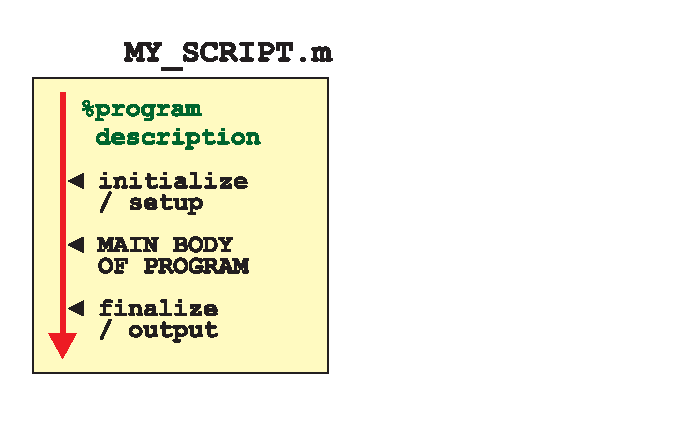
\includegraphics[width=\linewidth]{ch0-script.eps}
\caption{Schematic for a generic \textit{script}.}
\label{fig:ch0-script}
\end{marginfigure}

\begin{marginfigure}[-0.0in]
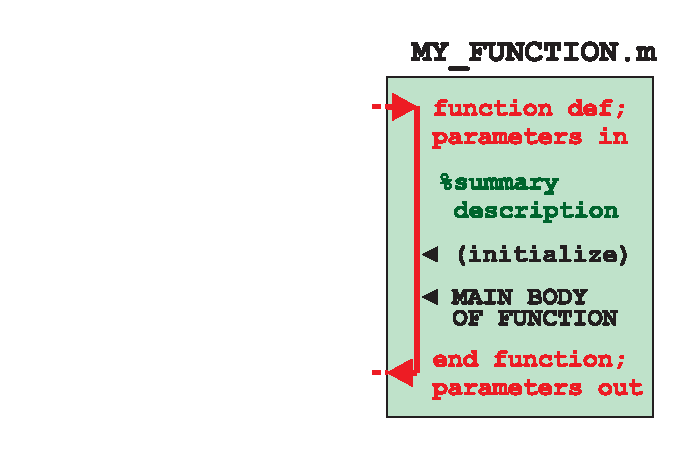
\includegraphics[width=\linewidth]{ch0-function.eps}
\caption{Schematic for a generic \textit{function}.}
\label{fig:ch0-function}
\end{marginfigure}

In these schematics, the flow (sequence) of the code is indicated by the red arrow. 

For the \textit{function}, that information is passed into the \textit{function}, and then returned back to where the function was called from, is indicated by the red arrows entering the top of the box and leaving the bottom of the box, respectively. (But note that there is no line of code at the end that tells the model to return values ... this is simply to illustrate the flow of the program, particularly when things get more complicated and there are multiple \textit{scripts} and \textit{functions} involved.)\sidenote[][0.0in]{All this should hopefully all become apparent later.}

For the \textit{script}, the code file starts with a comment (\textcolor[rgb]{0,0.501961,0}{\texttt{\%program description}}) summarizing what the \textit{script} does, although after the \textit{function} definition header line, so to should the \textit{function} (somewhere have comment lines describing what it does).

The black left-pointing filled triangles and associated text to the right, indicate categories of code content, and occurring in what order, that the programs might contain.

The purpose of these cartoons is to help you when faced with a blank page and the question: 'Where do I start' or 'What do I write' appears prominently in your mind\sidenote[][0.0in]{Also surrounded by flashing neon lights.}. It is to give you some sort of idea what bits might go where, and what general content is required in the file. The cartoons \uline{do not} (and are not intended) to show the exact details of the code content. Nor do they necessarily indicate all the different sections needed. Conversely, not all the sections illustrated may be strictly necessary and in come examples there may be nothing to 'initalize' and there may be no constants of local parameters to define the values of at the program start.

So please -- use the cartoons as a simple visual guide to the approximate structure of your program, but \uline{do not over-interpret them}.

%------------------------------------------------

\section{'Answer' codes}

For some of the more complex codes you will be expected to write, in addition to step-by-step instructions in the text, complete 'answer' codes will be provided at the back of the text. These are provided as guides to help you structure the code and see the 'bigger picture' of where all the parts fit together. The complete codes are obviously NOT provided for you simply to copy ... else you'll learn nothing. Except how to use the \textsf{CTRL-C} and \textsf{CTRL-V} key combinations.

Please use this provision as intended and for guidance only should you find yourself completely stuck.

%----------------------------------------------------------------------------------------

\mainmatter

%----------------------------------------------------------------------------------------
% CHAPTER 1
%----------------------------------------------------------------------------------------

\chapter{Introduction to numerical modelling}
\label{ch:01}

%------------------------------------------------

\newpage

%------------------------------------------------



%----------------------------------------------------------------------------------------
% CHAPTER 2
%----------------------------------------------------------------------------------------

\chapter{Numerical modelling -- zero-D / equilibrium}
\label{ch:02}

%------------------------------------------------

\newpage

%------------------------------------------------

\section{Zero-D Energy-balance model of the climate system}

In this Section, you are going to create, and then use in a series of applications, a zero-D equilibrium global 'climate model' --  the  simplest representation of the energy-balance   of the Earth's climate that it is possible to make. The model assumes that the climate system is always in balance, with no net gain or loss of energy, and hence that the energy absorbed from incoming (short-wave) solar radiation equals the (long-wave) radiative loss from the Earth's surface (or top-of-the-atmosphere) (Figure \ref{fig:ch8-blackbody}). The equations are outlined in the Box in the margin, and you'll need to rearrange them in terms of \(T\) (mean global surface temperature).

\marginnote[-2.5in]{\begin{mdframed}[backgroundcolor=light-blue,roundcorner=10pt,leftmargin=1, rightmargin=1, innerleftmargin=5, innerrightmargin=5, innertopmargin=5,innerbottommargin=5, outerlinewidth=1, linecolor=gray!10]
\textbf{Energy balance modelling (1)}
\\The surface energy budget at the Earths surface, to a zero-th order approximation, can be thought of as a simple balance between incoming, sort-wave radiation that is *absorbed*, and out-going, infra-red radiation.
\\On average (over the Earths surface and annually), the energy flux per unit area received from the sun, can be written:
\begin{docspecnormal}
\(F_{in} = \frac{(1-\alpha) \cdot S}{4}\)
\end{docspecnormal}
where \(S\) is the solar 'constant' which has a present-day value (given the notation \(S_{0}\)) of \( 1368 Wm^{-2}\)
\\(NOTE: the \(\frac{1}{4}\) appears because the cross-sectional area of the Earth is \(\frac{1}{4}\) of its total surface area -- i.e. you take energy intercepted by the Earth, which has an effective area of \(\pi\cdot r^{2}\), and spread it out over the entire surface -- an area of \(4\cdot\pi\cdot r^{2}\).)
\\Albedo (\(\alpha\)), is the fraction of incoming solar radiation that is reflected back to (-wards) space -- varies hugely across surface types (and angle of incoming radiation). A commonly used mean global approximation is to set: \(\alpha=0.3\).
\\Net outgoing infrared radiation proceeds according to black body emissions:
\begin{docspecnormal}
\(F_{out} = \epsilon \cdot \sigma \cdot T^{4}\)
\end{docspecnormal}
where \(\epsilon\) is the emissivity, \(\sigma\) is the Stefan-Boltzmann constant (in units of \(Wm^{-2}\)), and \(T\) the temperature in \uline{Kelvin} (\(K\)) (\(273.15 K == 0.0 \degree  C\)).
\\For a perfect black body radiator, we would set \(\epsilon\negthickspace=\negthickspace1.0\). However, it turns out that the Earth is not a smooth and perfectly matt black sphere radiating directly from the surface to space ... there is an atmosphere and water surface over \(\sim\)70\% of its surface etc etc. A common modification is then to reduce the effective emissivity of the surface to less than 1.0. A value of 0.62 is given in \textit{Henderson-Sellers} [2014], making the expression for the out-going flux: 
\begin{docspecnormal}
\(F_{out} = 0.62 \cdot \sigma \cdot T^{4}\)
\end{docspecnormal}
See Figure \ref{fig:ch8-blackbody}.
\end{mdframed}}

The exercises that follow are structured and you need to \uline{pay attention} to which \textbf{m-files} you are creating from scratch, which ones, having been created and coded up, you  do not then further edit, and which are \textit{functions} and which are \textit{script} files ... 

The sequence of work is as follows:

\begin{description}[align=right]

\setlength{\itemindent}{-0.2in}

\item [2.1.1] In this first Subsection ('\textit{The basic EBM}'), you'll  create a \textit{script} (\# \texttt{scr\_1\sidenote{This is not a suggested name of the \textbf{m-file}, but an ID to help you not get confused as to which script or function is being referred to in the text ...}}) \textbf{m-file} containing the Energy Balance Model (EBM), and test it.

\noindent (See Figure \ref{fig:ch8-schematic-scr1}.)

\item [2.1.2] Next, you'll turn your EBM \textit{script} (\texttt{scr\_1}) into a \textit{function} (\texttt{fun\_1})\sidenote{\textbf{Once the EBM function has been created, you do not at any point edit it any further!}} -- passing in the solar constant and albedo as parameters, and returning the surface temperature. (And test it.)

\noindent (See Figure \ref{fig:ch8-schematic-fun1}.)

\item [2.1.3] In the penultimate Subsection ('\textit{Calculating the evolution of the solar constant}'), you'll create a new function (\texttt{fun\_2}), which will take time (counted forward from the time of formation of the Sun) in \(Ga\), and return the value of the solar constant at that time (\(S(t)\) (\(Wm^{-2}\)) ).

\noindent (See Figure \ref{fig:ch8-schematic-fun2}.)

\end{description}

\noindent And then ...

\begin{description}[align=right]

\setlength{\itemindent}{-0.2in}

\item [2.1.4] ... finally (Subsection '\textit{Evolution of Earth's surface temperature}'), you'll create one last script (\texttt{scr\_4}), with a \textit{loop} in time in it, and from within this \textit{loop}, you'll call first the solar constant \textit{function} (\texttt{fun\_2}), taking time as an input and returning the value of \(S_{(t)}\), which you will then pass into the EBM (\# \texttt{fun\_1}),  taking  the value of \(S_{(t)}\) as input (along with albedo) and returning the surface temperature at time t --  \(T_{(t)}\).

\noindent (See Figure \ref{fig:ch8-schematic-scr4fun1fun2}.)

\end{description}

\newthought{\textbf{\textcolor{red}{OPTIONAL}} -- model parameter sensitivity / loop exercises:} \\\noindent You can also take the EMBM function (now ignoring the solar constant function), and play some theoretical games with it in order to understand how sensitive global surface temperature is to key variables (solar constant and albedo):

\begin{description}[align=right]

\setlength{\itemindent}{-0.2in}

\item [2.1.5] In the Subsection '\textit{Parameter sensitivity experiments using the EBM -- \#1}', you will create a new script (\texttt{scr\_2}) with a single loop in it. Within the loop, you will make a call to the EBM function (\# \texttt{fun\_1}) that you created.\sidenote{DO\ NOT put code the loops into the EBM function -- leave the function alone ...}

\noindent (See Figure \ref{fig:ch8-schematic-scr2fun1}.)

\item [2.1.6] Then, in '\textit{Parameter sensitivity experiments using the EBM -- \#2}' -- an extension to the previous Subsection work, you will create another new script (\texttt{scr\_3}), this time  with a double (nested) loop in it. As before -- within the loop, you will make a call to the EBM function.
Note that there is going to something of a diversion in this Subsection that will further help illustrate nested loops for you.

\noindent (See Figure \ref{fig:ch8-schematic-scr3fun1}.)

\end{description}

%------------------------------------------------

\newpage

\subsection{The basic EBM}

\begin{marginfigure}[-0.0in]
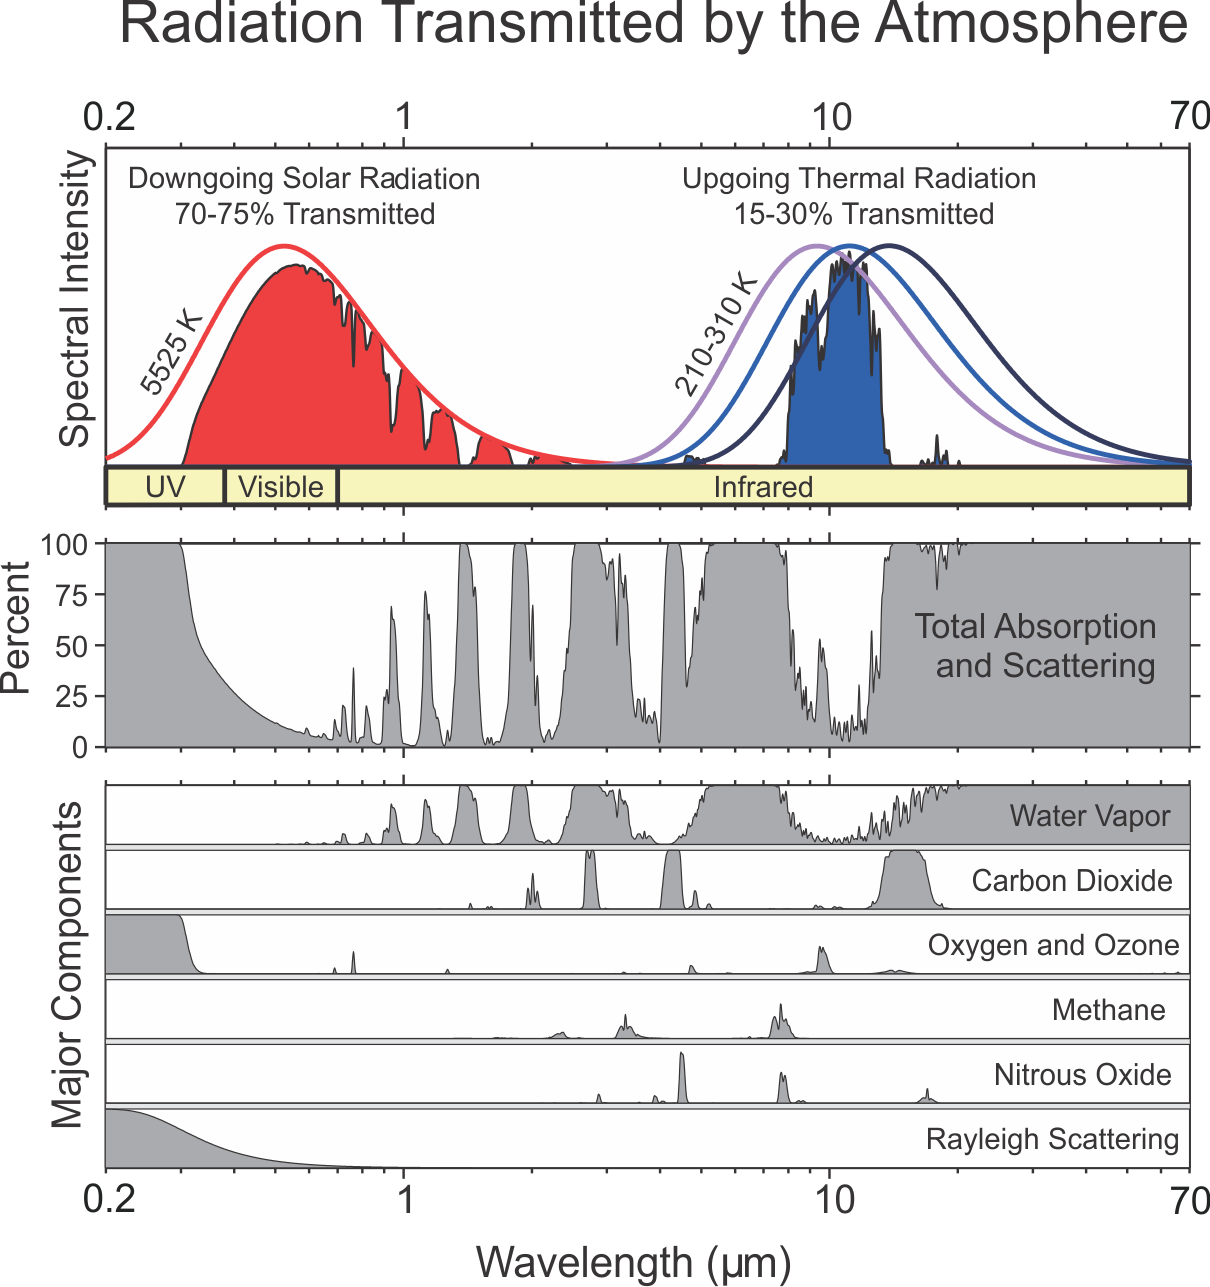
\includegraphics[width=\linewidth]{ridgwell-and-valdes-Figures.png}
\caption{The pattern of absorption bands generated by various greenhouse gases and aerosols (lower panel) and how they impact both incoming solar radiation (upper left) and outgoing thermal radiation from the Earths surface (upper right). (Figure prepared by Robert A. Rohde for the Global Warming Art project.).}
\label{fig:ch8-blackbody}
\end{marginfigure}

To kick off -- create a new \textit{script} (\textbf{m-file}) ('\texttt{scr\_1}' in the summary notation) and code up the analytical solution to the basic global mean energy budget at the surface of the Earth (see Box) in a program structure illustrated schematically in Figure \ref{fig:ch8-schematic-scr1}.\sidenote[][0.0in]{
Note that the code is relatively simple and does not involve (yet) loops or conditionals or anything like that. Although ... I am sure it will involve lots of nice juicy comments and sensible variable names(?) \\Simply set up the values of the various constants and parameters you need at the start of the code, then solve for \(T\) at the end of the code. The structure (omitting \textcolor[rgb]{0,0.501961,0.25098}{\texttt{\% comments}}) of your code may look like:
\begin{docspecmargin}
\textcolor[rgb]{0,0.501961,0.25098}{\% section for constants (variables you do not expect ever to change)}
\\\ldots
\\\textcolor[rgb]{0,0.501961,0.25098}{\% section for parameters (variables you might adjust)}
\\\ldots
\\\textcolor[rgb]{0,0.501961,0.25098}{\% solve for T}
\\\(T = \ldots\)
\end{docspecmargin}
} The equations for in-coming and out-going radiation (energy) were given previously. You simply need to re-arrange these in terms of \(T\) (i.e. \(T=...\)) and write them as code. This will form the basis of subsequent, more complex (and later, time-stepping) models. In detail:

You are given:
\begin{docspecnormal}
\(F_{in} = \frac{(1-\alpha) \cdot S}{4}\)
\end{docspecnormal}
and
\begin{docspecnormal}
\(F_{out} = \epsilon \cdot \sigma \cdot T^{4}\)
\end{docspecnormal}
and are told at at equilibrium:
\begin{docspecnormal}
\(F_{in} = F_{out}\)
\end{docspecnormal}
You can then  write:
\begin{docspecnormal}
\(\frac{(1-\alpha) \cdot S}{4} = \epsilon \cdot \sigma \cdot T^{4}\)
\end{docspecnormal}

\noindent You  task is then to re-arrange this equation in terms of \(T\) -- do this first \uline{on paper} before worrying about any code.

\noindent How to write the math down as \textbf{MATLAB} code? For the first part (\(F_{in}\)), we could e.g. write:
\begin{docspec}
Fin = ((1-albedo)*solar\_constant)/4;
\end{docspec}
This pretty well much as you would write as math (on paper) with the exception of the variables having much longer names than you would typically use in math (where often Greek characters, with or without sub- or super-scripts, are used). Here, \texttt{albedo} and \texttt{solar\_constant} are variables holding the values of planetary albedo and solar constant, and the result of the calculation is assigned to a variable \texttt{Fin}. For completeness, you would define these values, e.g.
\begin{docspec}
albedo = 0.3; \textcolor[rgb]{0,0.501961,0}{\% initial albedo assumption}\\
solar\_constant\ = 1368.0; \textcolor[rgb]{0,0.501961,0}{\% set modern solar constant}\\
Fin = ((1-albedo)*solar\_constant)/4; \textcolor[rgb]{0,0.501961,0}{\% energy in}
\end{docspec}
(and you might add to the comments, to include the units for each variable).

\noindent For writing out the \(F_{out}\) part of the equation in code, you will need to find (from the Internet?) the value of the (Stefan-Boltzmann) constant. When you have found this, assign this value\footnote{Obviously, in this example, this is NOT the actual value ...} to a variable, e.g.
\begin{docspec}
sb\_constant = 9.9999E19;
\end{docspec}

\noindent ... and \uline{you will need to be careful with units of this} (Wikipedia, for example, will provide the Stefan-Boltzmann in a variety of units). Use a 'dimension' check to see if you have the units correct. This works as follows:

In the equation:
\begin{docspecnormal}
\(F_{out} = \epsilon \cdot \sigma \cdot T^{4}\)
\end{docspecnormal}
-- on the left hand side we have units of \(W m^{-2}\), and on the right hand side \(\epsilon\), the emissivity, is dimensionless, and \(T^{4}\) has units of ... \(K^{4}\). The Stefan-Boltzmann constant, \(\sigma\), must be in units that balance this, i.e. \(W m^{-2} K^{-4}\), such that:
\begin{docspecnormal}
\(W m^{-2} == [] \cdot\ W m^{-2} K^{-4} \cdot\ K^{4}\)
\end{docspecnormal}
(where \([]\) is indicating no dimension (units) for \(\epsilon\)).

Also note in the context of the Stefan-Boltzmann constant, \(\sigma\), how scientific notation (floating point) numbers are dealt with in \textbf{MATLAB}. For example, while in normals maths speak, you might write:
\begin{docspecnormal}
\(x = 9.9999\times 10^{19}\)
\end{docspecnormal}
in \textbf{MATLAB} you would write:
\begin{docspec}
x = 9.9999E19
\end{docspec}
although, you could also write this out long-hand and more like the maths speak version \(x = 9.9999\times 10^{19}\), if you prefer, e.g.
\begin{docspec}
x = 9.9999*10\(^{\wedge}\)19
\end{docspec}
(There are equivalent representations, although the 1st one is more compact and hence less prone to errors (bugs).)

\begin{marginfigure}[0.0in]
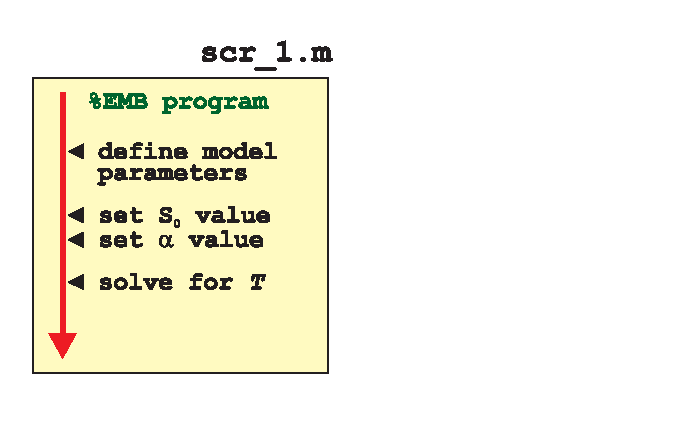
\includegraphics[width=\linewidth]{ch8-schematic-scr1.eps}
\caption{Form of the basic EBM model.}
\label{fig:ch8-schematic-scr1}
\end{marginfigure}

\vspace{1mm}
\noindent\rule{4cm}{0.5pt}
\vspace{2mm}

\noindent So coming back to what exactly you need to do in your \textbf{m-file} -- writing down in \textbf{MATLAB} an equation for \(T\) (\texttt{temp}) -- you can either write this out in full in a single line, or make use of the code for \texttt{Fin}, and build on that. For the latter option, knowing that \(F_{in} = F_{out}\), you should be able to see from the equation for \(F_{out}\), that if you divide \(F_{in}\) by \(\left(\epsilon\cdot\sigma\right)\) (or divide by \(\epsilon\), then divide by \(\epsilon\)), that you will be left with the 4th power of \(T\). You then need to take the \(\frac{1}{4}\) root of that, which you can write in \textbf{MATLAB} as:
\begin{docspec}
temp = temp4\(^{\wedge}\)0.25;
\end{docspec}
or if you prefer:
\begin{docspec}
temp = temp4\(^{\wedge}\)(1/4);
\end{docspec}
(where I am assuming that temp4 is the partially re-arranged equation that gives the 4th power of \(T\)).

For now in your \textit{script} \textbf{m-file} -- prescribe the value of \(S\) (variable: \texttt{solar\_constant}) -- for which the modern value is 1368 Wm\(^{-2}\) (\(S_{0}\)) as well as the value of planetary albedo (\(\alpha=0.3\), variable: \texttt{albedo}) -- somewhere near the start of the program (see Figure \ref{fig:ch8-schematic-scr1}).

\vspace{1mm}
\noindent\rule{4cm}{0.5pt}
\vspace{2mm}

\noindent Now run it.

If you did not screw-up the units on the Stefan-Boltzmann constant, then you should have an equilibrium (global, annual mean) surface temperature of around 14\degree C\sidenote{Remembering to convert from Kelvin (\(K\)) to degrees Centigrade (\degree C). In the equation you have re-arranged, \(T\) is in units of Kelvin (\(K\)).} ... If not -- debug. Assuming that the code ran without errors but gave a nutty answer, try the following fault-finding sequence:
\begin{enumerate}[noitemsep]
\setlength{\itemindent}{.2in}
\item Check that the units are correct!!!
\item Check that the equation has been re-arranged correctly -- a common source of errors is incorrect placement of parentheses ... or not placing parentheses around multiple variables you are divining something all by.
\\ If it helps you to avoid confusion and potential errors and bugs by breaking down calculations into multiple steps using temporary/intermediate variables and partial calculations ... then do it!
\item If still 'no' -- maybe take the 2 component equations (for \(F_{in}\) and \(F_{out}\)), plug \(S\) into the equation for \(F_{in}\) and then play with different values of \(T\) to find a value for \(F_{out}\) that is approximately equal -- is the value for \(T\) sane? If not, double-check the units and values in both component equations.
\end{enumerate} 

\noindent Once it is working, have a quick play about, changing the value of \(S\) and albedo (\(\alpha\)) (saving the \textbf{m-file} each time and re-running) to get a vague feel for how sensitive the surface temperature is to these two parameters.

%------------------------------------------------
%
\newpage

\subsection{The EBM as a function}

\begin{marginfigure}[0.125in]
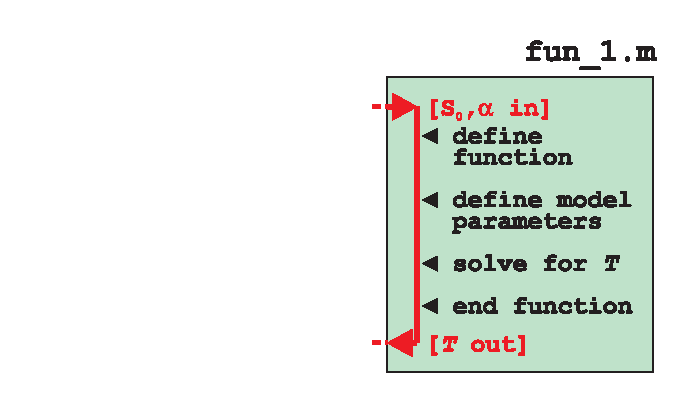
\includegraphics[width=\linewidth]{ch8-schematic-fun1.eps}
\caption{Form of the basic EBM model as a \textit{function}.}
\label{fig:ch8-schematic-fun1}
\end{marginfigure}

We'll now make your model more flexible so that it can be applied to the subsequent Examples. So -- turn it into a \textit{function}\sidenote[][0.25in]{
Refer to earlier in the text and also \textbf{help} on the required structure/syntax of a \textit{function}. Recall the basic structure of a function \textbf{m-file}, has as its \uline{VERY\ FIRST\ LINE}:
\begin{docspecmargin}
\textcolor{blue}{function} [OUT] = ... 
\\ \ \ \ FUNCTION\_NAME(IN)
\end{docspecmargin}
where \texttt{OUT} represents one (or more) variables that are passed out (the 'result' of the function), \texttt{FUNCTION\_NAME} is the name of your function, and \texttt{IN} is the name (or names, comma-separated) of one (or more) variables (parameter values) that are passed into the function. (The very last line of the function should have an \textcolor{blue}{end}.)
\\For example, to pass in two variables, \texttt{IN\_1} and \texttt{IN\_2}, you'd have:
\begin{docspecmargin}
\textcolor{blue}{function} [OUT] = ... 
\\ \ \ \ FUNCTION\_NAME(IN\_1,IN\_2)
\end{docspecmargin}
} that takes in 2 parameters -- the solar constant (\(S\)) and the mean global planetary albedo (\(\alpha\)) (see hint in the margin!!). The \textit{function} should return the global mean surface temperature, \(T\).\sidenote{Note that the parameters passed into, and returned by, the function, can be called anything you want. As long as they are useful (and clearly defined/explained in a comment somewhere).} (See Figure \ref{fig:ch8-schematic-fun1}) Remember that you can directly replace the symbols in an equation with variable names in \textbf{MATLAB}, e.g.
\begin{itemize}[noitemsep]
\setlength{\itemindent}{.2in}
\item[] \(S \rightarrow\) \texttt{solar\_constant}
\item[] \(\alpha\ \rightarrow\) \texttt{albedo}
\item[] \(T \rightarrow\) \texttt{temp}
\end{itemize}
(or whatever you like, as long as the names help you in the coding and debugging).
Or if you prefer -- create a new (empty) \textit{function} (select \textsf{New} and then \textsf{Function} from the \textbf{MATLAB} toolbar/menu-bar) and then copy-paste in the contents of \textsf{scr\_1.m}. Note that in your new \textit{function} version of the program, you no longer define  the values for \texttt{solar\_constant} and \texttt{albedo} in the \textbf{m-file} -- instead, these values are passed into the \textit{function} when you call it. For instance, if at the top of the \textit{function} (see side-note) you  defined:
\begin{docspec}
\textcolor{blue}{function} [temp] = fun\_1(solar\_constant, albedo)
\end{docspec}
then when you call the \textit{function}  at the command line:
\begin{docspecbold}
>> fun\_1(1368.0,0.3)
\end{docspecbold}
you are passing in the value \(1368\) (\(Wm^{-2}\)) -- assigned to the variable \texttt{solar\_constant} (in \textsf{fun\_1.m}), and the value \(0.3\) (dimensionless) --  assigned to the second variable in the \textit{function} definition (\texttt{albedo}). The \textit{function} then returns whatever value you have calculated and assigned to the variable \texttt{temp}, back to you (and which then appears at the command line).

Try playing with the \textit{function} in the same way as before, but now passing the different values of \(S\) and \(\alpha\) (rather than having to edit the \textsf{m-file}, save, and re-run each time). To use the \textit{function} (assuming you called it e.g. \texttt{fun\_1}), and assuming the 2 passed parameters are in the order: \(S\), \(\alpha\) and are given their default values, you'd write (at the command line):
\begin{docspecbold}
>> temp = fun\_1(1368.0,0.3);
\end{docspecbold}
(and get a value close to 14\degree C returned and assigned to the variable \texttt{temp}, and if not -- debug it ...).

%------------------------------------------------

\newpage

\subsection{Creating a function for the evolution of solar constant through geological time}

In this  sub-subsection, and as a precursor to simulating how Earths surface temperature may have changed through geological time, you are going to code up a new \textit{function} that calculates (and returns) the value of the solar constant as a function of time.

So far you only have a function equating solar constant (\(S\)) to temperature (\(T\)). What you need is some way of equating time (\(t\)) to the value of the solar constant at that time \(S_{(t)}\) (which you can then turn into temperature). We'll remedy this toot sweet.

Start by creating a new  (blank) \textbf{m-file} and define it as a \textit{function} that takes in a variable for time, \(t\) (in units of \(Ga\)) and spits out  (aka, returns) the calculated value of \(S_{(t)}\) (\(Wm^{-2}\)) (this \textit{function} will be '\texttt{fun\_2}' in the on-going notation and obviously saved as \textsf{fun\_2.m}). i.e., your \textit{function} definition (at the top of the \textbf{m-file}) will look something like:
\begin{docspec}
\textcolor{blue}{function} [St] = fun\_2(t)
\end{docspec}
where now I am shortening the variable name for the solar constant (to '\texttt{S}') and then adding a '\texttt{t}' to remind me that it is a time-dependent value (hence \texttt{St} rather than e.g. \texttt{solar\_constant\_time}). The code structure you are aiming for is illustrated in Figure \ref{fig:ch8-schematic-fun2}.

\marginnote[-3.875in]{\begin{mdframed}[backgroundcolor=light-blue, roundcorner=10pt,leftmargin=1, rightmargin=1, innerleftmargin=5, innerrightmargin=5, innertopmargin=5,innerbottommargin=5, outerlinewidth=1, linecolor=light-gray]
\textbf{Solar constant}
\\The long-term evolution of solar luminosity \(L_{t}\) as a function of time \(t\) can be approximated [\textit{Gough} [1981]; \textit{Feulner} [2012]) by:
\begin{docspeclarge}
\(\frac{L_{t}}{L_{0}} = \frac{1}{1+\frac{2}{5}\cdot (1-\frac{t}{t_{0}})}\)
\end{docspeclarge}
where \(t_{0}\) is the age of the sun -- 4.57 Gyr (4.57\(\times\)10\(^{9}\) yr) and \(L_{0}\) is the present-day solar luminosity (3.85\(\times\)10\(^{26}\) W).
\\The value of \(L_{0}\) is equivalent to a flux (\(Wm^{-2}\)) of 1368 Wm\(^{-2}\) incident at the top of the atmosphere at Earth -- the present-day solar 'constant' \(S_{0}\). In the equation, \(L\) can hence be substituted for \(S\) to give the value of \(S\) (\(Wm^{-2}\)) at any time (\(S_{(t)}\)), i.e.
\begin{docspeclarge}
\(\frac{S_{(t)}}{S_{(t=0)}} = \frac{1}{1+\frac{2}{5}\cdot (1-\frac{t}{t_{0}})}\)
\end{docspeclarge}
or, in terms of the value of \(S\) at time \(t\) and using using the notation \(S_{0}\) in place of \(S_{(t=0)}\):
\begin{docspeclarge}
\(S_{(t)} = \frac{S_{0}}{1+\frac{2}{5}\cdot (1-\frac{t}{t_{0}})}\)
\end{docspeclarge}
Note that in the formula, \(t\) is counted (in Gyr) relative to the formation of the Sun (i.e. present-day would be: \(t=4.57\)). 
\\The reference value of \(t\): \(t_{0}\), is \(t_{0}=4.57\) Gyr.
\\The reference value of \(S\): \(S_{0}=1368\) Wm\(^{-2}\).
\end{mdframed}}

\begin{marginfigure}[0.0in]
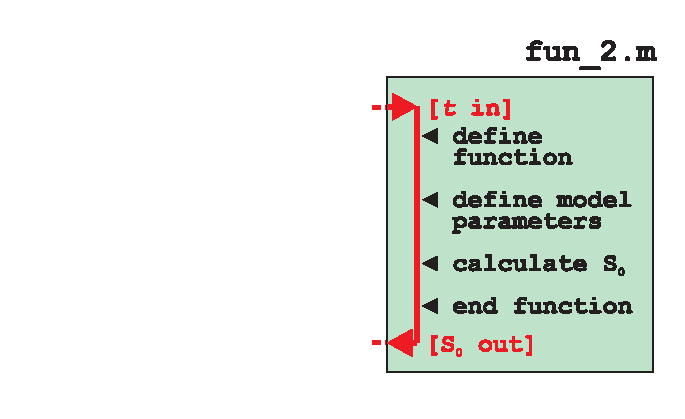
\includegraphics[width=\linewidth]{ch8-schematic-fun2.eps}
\caption{Schematic structure of code for calculating the solar constant (output) as a function of time (input).}
\label{fig:ch8-schematic-fun2}
\end{marginfigure}

The background to the equation that will go into your function is given in the Solar constant Box. In this, you'll first need to substitute the modern value of the solar constant (\(S_{(t=0)}\) or \(S_{0}\)) into the equation to leave it in terms of \(S_{(t)}\) (the solar constant value at time \(t\)).
 
Your function, aside from the all-important 1st line (and \textcolor{blue}{\texttt{end}} at the end) and appropriate \textcolor[rgb]{0,0.501961,0.25098}{\texttt{\% comments}}, need have little more in than a definition for any constant you might want to use, such as the modern value of \(S_{(t=0)}\) and perhaps the reference time\sidenote[][0.0in]{Which is also equal to the current time (since the formation of the Sun).} (\(t_{0}\)) (4.57 Ga) ... followed by a single line for the equation giving the value of \(S_{(t)}\):
\begin{docspeclarge}
\(S_{(t)} = \frac{S_{0}}{1+\frac{2}{5}\cdot (1-\frac{t}{t_{0}})}\)
\end{docspeclarge} 

As before -- your primary task is to convert this equation into \textbf{MATLAB} code. 

To do this, you could either create parameters (variables) containing the values of \(S_{0}\) and \(t_{0}\) (better), e.g.
\begin{docspec}
ref\_S0 = 1368.0;\\
ref\_t = 4.57;\\
\end{docspec}
and use the variable names in the code in place of actual (constant) values, e.g.:
\begin{docspec}
St = ref\_S0 / ( ... )
\end{docspec}
or (less good from a programming perspective), plug them directly into the code, e.g.
\begin{docspec}
St = 1368.0 / ( ... )
\end{docspec}
Regardless of which approach you take, remember that the variable \texttt{t} that is is passed in as per defined in the \textit{function} header (see above), will need to appear in your equation.

The result of the equation -- the value of the solar constant at that time, is then assigned to the variable \texttt{St} and passed out as the result of the function (again, as per the function definition/header).

In the code and in general -- use as many pairs of (nested) parentheses as you need to help make the equation clear. You can also use spaces to help make it clearer which end parenthesis corresponds to which opening parenthesis

When you think you have done this -- check it -- plug in some values of time into your function, i.e.
\begin{docspecbold}
>> St = fun\_2(4.57);
\end{docspecbold}
In this example, should return a value of \(1368\) (\(Wm^{-2}\)) which is assigned to the variable \texttt{St}.

\vspace{1mm}
\noindent\rule{4cm}{0.5pt}
\vspace{-2mm}

\newthought{\textbf{\textcolor{red}{OPTIONAL}} -- As a test --} see if you can adjust your \textit{function} (but save it under a different/new name so as to retain a copy of the original) so that rather than passing in time, measured since the formation of the Sun, you pass in time relative to now (i.e. \texttt{>> fun\_2(0.0)} would then give you a value of \(1368\)).
Hint: the time used in the equation, must be as Gyr following the formation of the sun, but the value you are passing in, has had a value of 4.57 (Ga) removed from it to make it relative to now. Hence, before the calculation in the \textit{function}, you need to add this value back to the time variable passed in, to make it absolute rather than relative time again.

%------------------------------------------------

\newpage

\subsection{Putting it all together -- using multiple functions to calculate global surface temperature as a function of geological time}

Finally ... you are going to bring it all together and plot the evolution of the surface temperature of the Earth, at 100 Myr intervals,  spanning approximately the age of the Earth and much of its potential long-term future.

Start by creating a new (yet another blank \textbf{m-file}) \textit{script} ('\texttt{scr\_4}')\footnote{The structure of the overall program is shown in  Figure \ref{fig:ch8-schematic-scr4fun1fun2}.}. You are going to need a loop in time (e.g. with the variable name \texttt{t}), perhaps looping from 0.0 (the age of formation of the Sun) to 10.0 Ga (with the step size being 0.1 Ga). \uline{Within the time loop}, you will:

\begin{enumerate}[noitemsep]
\setlength{\itemindent}{.2in}
\vspace{1mm}
\item Pass to your solar constant \textit{function} (\texttt{fun\_2.m}) your  variable containing the current value of time (\texttt{t}), and obtain the corresponding value of the solar constant (\(S_{(t)}\)), and assign to a variable e.g. \texttt{St}.
\\Note that you do not copy-paste the \textsf{fun\_2.m} code into \textsf{scr\_4.m} ... you simply call the \textit{function} within the loop exactly as per you did at the command line (but assign the result to a variable), e.g.
\begin{docspec}
St = fun\_2(t);
\end{docspec}
(NOTE: The summary figure (Figure \ref{fig:ch8-schematic-scr4fun1fun2}) is intended to indicate the flow of information (variable values) and relationship between the \textit{script} and two \textit{functions} \textbf{m-files}, rather than that the code for the 2 functions should be embedded (which it should not) within the actual \textit{script} file itself ...)
\vspace{1mm}
\item  Call your zeroD EBM \textit{function} (\texttt{fun\_1.m}) to calculate the corresponding surface temperature, passing it the value of \(S_{(t)}\) that you have just calculated and assigning the result to  e.g. \texttt{temp}:
\begin{docspec}
temp = fun\_1(St,albedo);
\end{docspec}
(or simply replace \texttt{albedo} with a fixed value, e.g. 0.3).
\vspace{1mm}
\item Store in an array, or pairs of vectors, the current time in the loop alongside the corresponding value of \(T\). For hints on the various different possibilities in doing this see earlier in the text, but you might e.g. do something like:
\begin{docspec}
vt = [vt t];\\
vtemp = [vtemp temp];
\end{docspec}
(having first (before the loop) initialized these vectors as empty, e.g. \texttt{vt=[];} and \texttt{vtemp=[];}), which will append the current time to  vector\texttt{vt}, and at the same row number, the current temperature to vector \texttt{vtmp}.
\end{enumerate}
\vspace{-1mm}
Once the loop has completed, plot surface temperature (\textit{y}-axis) as a function of time (\textit{x}-axis).

\begin{marginfigure}[-6.0in]
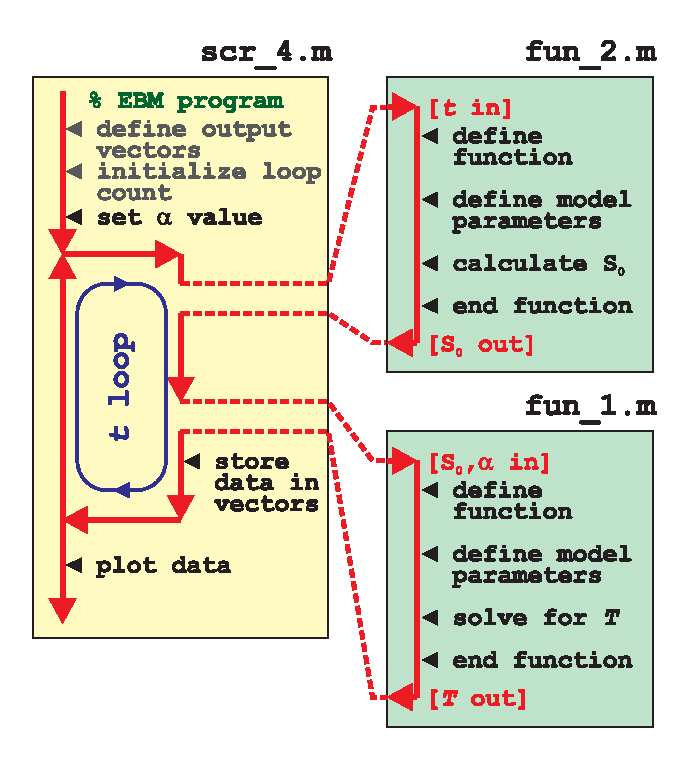
\includegraphics[width=\linewidth]{ch8-schematic-scr4fun1fun2.eps}
\caption{Schematic of the evolution of surface temperature over geological time program, and relationship between main program script, and solar constant and EBM functions. \uline{Note} -- in this schematic, the code contents of the two \textit{functions} remain in their respective \textbf{m-files}. The \textit{function} code \uline{does not} get copy-pasted into the \textsf{scr\_4.m} script file. The red arrows indicate the passing of variable values ... from \textsf{scr\_4.m} into each \textit{function}, with the \textit{functions} returning variable values back to \textsf{scr\_4.m}.}
\label{fig:ch8-schematic-scr4fun1fun2}
\end{marginfigure}

Likely bug possibilities include mistakes with nested parentheses \texttt{(())}, units (e.g. \(K\) vs. \(\degree C\)), and time, which  should run forward from zero (the formation of the Sun). A schematic of the program structure is shown in Figure \ref{fig:ch8-schematic-scr4fun1fun2} to aid you.

Assuming that you have managed something like Figure \ref{fig:ch8-ebm-solarconst}\sidenote[][-1.0in]{Note that a line has been added to highlight \(t=0\) (i.e. the present-day) -- see \docenv{line} (see earlier). This plot also has an altered time-axis and time is plotted relative to now -- see below.} -- what strikes you, in light of (hopefully) what you know about the past history of climate and evolution of life on this planet, about your model projection (for the past)? What is 'missing'?

\begin{marginfigure}[-0.0in]
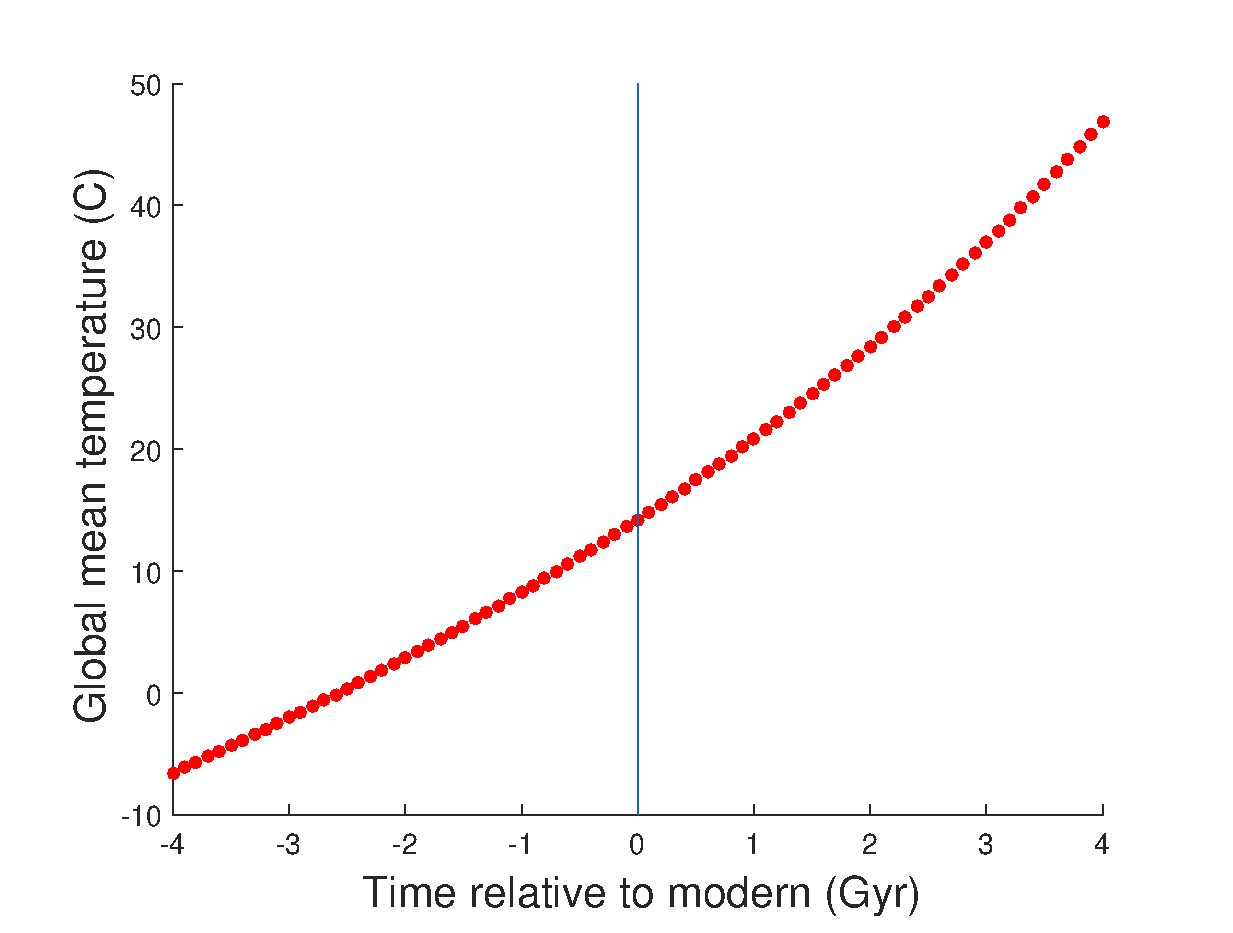
\includegraphics[width=\linewidth]{ch8-ebm-solarconst.eps}
\caption{Simple EBM projection of the evolution of Earth surface temperature with time. Time at the present-day is highlighted by a vertical line (drawn using the \textbf{MATLAB} \docenv{line} function).}
\label{fig:ch8-ebm-solarconst}
\end{marginfigure}

As an additional step and noting that the time-scale is not entirely helpful in terms of knowing when 'now' is, you could:

\begin{enumerate}
\vspace{-0mm}
\item Draw on a vertical line (\texttt{hold on}) at 4.57 ('now', relative to the time of formation of the Sun).
\vspace{-1mm}
\item Transform the \textit{x}-axis time scale to \uline{time relative to now} (as shown in Figure \ref{fig:ch8-schematic-scr4fun1fun2}). 
\\To do this -- as you loop through time relative to the formation of the Sun, when you save the current time for plotting, you could subtract 4.57 from the loop value before passing it to \texttt{fun\_2.m}.
\vspace{-1mm}
\item Or ... you could save the time as given in the loop, but transform the \textit{x}-axis time scale to time relative to now by subtracting a value of 4.57 when you come to \texttt{plot} it, e.g.:
\vspace{-1mm}\begin{docspec}
>> plot(x-4.57,y);
\end{docspec}\vspace{-1mm}
or more explicitly so you can see what is going on:
\vspace{-1mm}\begin{docspec}
>> plot((x(:)-4.57),y(:));
\end{docspec}\vspace{-1mm}
\end{enumerate}
Note that you do not have to plot the entire dataset and could set the x-axis limits to e.g. \(-4 \rightarrow\ +4\) Gyr relative to present (again as per the example in Figure \ref{fig:ch8-schematic-scr4fun1fun2})..

%------------------------------------------------
%------------------------------------------------

\newpage

\subsection{Parameter sensitivity experiments using the EBM -- \#1}

[Note that in this section, variables names are shortened and simplified as compared to before, with \texttt{S} replacing\texttt{ solar\_constant}, and \texttt{T} replacing \texttt{temp} (and then \texttt{a} replacing \texttt{albedo}). Feel free to retain the previous (or whatever you like) naming convention.]
\vspace{2mm}

\noindent Common in numerical modelling is quantifying how sensitive a system is to the choice of parameter values -- called a \textit{sensitivity experiment}. You may already have gotten a feel for roughly how sensitive \(T\) was to changing \(S\) on its own, or changing \(\alpha\) on its own, but what about when both parameters vary together? In this exercise you are going to utilize your energy-balance model \textit{function} ('\texttt{fun\_1}' in the summary notation) to explore this.

Create a new blank script ('\texttt{scr\_2}') and define 2 parameters near the start of the \textbf{m-file} -- one for the value of \(S\) and one for the albedo, \(\alpha\), then further down the code, call your function (\texttt{fun\_1}), passing it these 2 parameters \uline{but remembering} that you need to assign the result of your function (\texttt{fun\_1}) to some \textit{variable}\sidenote{i.e.
\begin{docspecmargin}
T = fun\_1(S,a);
\end{docspecmargin}assigns the result of your temperature calculation to the variable \texttt{T}.}. So far so boring, as this is in effect what you had been doing previously in 'playing' with the energy balance function. 


Starting with a simple 1-D case and considering  a progression of different values of \(S\), you are going to need to create a loop\sidenote{You are going to put the loop in the script (\# \texttt{scr\_2}), NOT the function (\# \texttt{fun\_1}).

\textbf{An entire plane of Hell is reserved for anyone coding the loop in the function.}
}. There are two/three ways of constructing the loop\sidenote{In both cases a \texttt{for ...} loop.}:

\begin{enumerate}
\setlength{\itemindent}{.65in}

\item [\textbf{loop option \#1}] You could loop directly through the range of values of \(S\) that you are interested in, e.g.
\begin{docspec}
\textcolor{blue}{for} S = 1000:100:1500
\\ \ \ \ \ \textcolor[rgb]{0,0.501961,0}{\% CODE GOES HERE}
\\\textcolor{blue}{end}
\end{docspec}
in which case, \(S\) will go from 1000 to 1500 (\(Wm^{-2}\)) in steps of 100 (\(Wm^{-2}\)) \sidenote{You can pick a different range and increment ... this is just a quasi-random example to illustrate ...}.
\\Perhaps a little inconveniently, this does not pass exactly through the modern value (1368 Wm\(^{-2}\)), although when you plot as a continuous line (e.g. in \texttt{plot}),  maybe this does not matter.  Remember, you could also interpolate the result later (e.g. on a new vector of solar constant values that include \texttt{1368}).

You could have addressed this by constructing a slightly less convenient form of the loop, e.g.:
\begin{docspec}
\textcolor{blue}{for} S0 = 1068:100:1568
\\ \ \ \ \ \textcolor[rgb]{0,0.501961,0}{\% CODE GOES HERE}
\\\textcolor{blue}{end}
\end{docspec}
which now passes exactly through the modern value of \(S\).

Or ... you could have made the loop go around in steps of \texttt{1} (and hence passing through a value of \texttt{1368}) for a total of 501 loop iterations(!) But this is over-kill in terms of data generation if the calculated equilibrium is  not  particularly sensitive to the value of solar constant (i.e. not highly non-linear).

\item [\textbf{loop option \#2}] Alternatively, you could have an integer count for the loop, and then derive a  value of \(S_{0}\) from this. For example:
\begin{docspec}
S\_modern = 1368.0;
\\\textcolor{blue}{for} m=-5:5
\\ \ \ \ \ S = S\_modern + 100*m
\\ \ \ \ \ \textcolor[rgb]{0,0.501961,0}{\% CODE GOES HERE}
\\\textcolor{blue}{end}
\end{docspec}
Look carefully through this code and follow what is going -- as \texttt{m} counts from \texttt{-5} to \texttt{5} (in steps of\texttt{ 1}), \texttt{100} times the value of \texttt{m} is added to the modern value of \(S\) (\(S_{0}\)) \sidenote{The variable definition \texttt{S0\_modern = 1368.0} at the top of the code fragment.}, meaning that \(S\) ends up going from \texttt{S0\_modern} - 500, to \texttt{S0\_modern} + 500 Wm\(^{-2}\) (in steps of 100 Wm\(^{-2}\)).

\item [\textbf{loop option \#3}]
Or ... as a variant on \#2:
\begin{docspec}
S\_modern = 1368.0;
\\\textcolor{blue}{for} m=1:11
\\ \ \ \ S = S\_modern + 100*(n - 6)
\\ \ \ \ \textcolor[rgb]{0,0.501961,0}{\% CODE GOES HERE}
\\\textcolor{blue}{end}
\end{docspec}
which does exactly the same (do a mental check on this)  but now counts \texttt{m} starting from a value of \texttt{1}.

\end{enumerate}

\noindent To practice your coding skills -- try coding up all 3 variants and satisfy yourself that you are happy how they all work, and how they are all equivalent to each other.

So what does it matter, and/or is one 'better' than the others? Although the all are  in effect equivalent, the advantage with the second (and third versions) is that you explicitly have an integer counter. For the first version, you'd have to add lines, e.g.:
\begin{docspec}
count = 0;
\\\textcolor{blue}{for} S = 1068:100:1568
\\ \ \ \ count = count + 1;
\\ \ \ \ \textcolor[rgb]{0,0.501961,0}{\% CODE GOES HERE}
\\\textcolor{blue}{end}
\end{docspec}
in order to have a loop count.

And why might we want some sort of an integer counter in the first place? Well, you might want to save the data, i.e. the calculated (by your function) value of \(T\) vs. the inputted value of \(S\). This data will need to go into an array, with one row corresponding to each value of \(S\).

As per constructing the loop itself, there are  also multiple (two-and-a-bit) obvious alternative ways of saving the data (and assigning calculated values to sequential locations in an array):

\begin{enumerate}
\setlength{\itemindent}{.65in}

\item [\textbf{save option \#1}] In this, you create the necessary array(s) beforehand, e.g. using the \texttt{zeros} \textit{function}. For instance, to create a vector with 11 rows (and 1 column), suitable for saving the value of \(T\) calculated by each call to your EBM function (\textsf{fun\_1.m}), you could write:
\begin{docspec}
data\_T = zeros(11,1);
\end{docspec}
which would create a (single) column vector with 11 rows. You'd also need an equivalent vector (e.g. \texttt{data\_S} in this example) for storing the corresponding value of \(S\) used in the temperature calculation. These vectors are created before the loop starts.
\\Then, within the loop (and after the calculation of \(T\)), you'd assign your values of \(S\) and \(T\) by using whichever index you created\sidenote{i.e. which of the loop OPTIONS you chose earlier.}:
\begin{docspec}
\ \ \ data\_S(m) = S;
\\ \ \ \ data\_T(m) = T;
\end{docspec}
or:
\begin{docspec}
\ \ \ data\_S(count) = S;
\\ \ \ \ data\_T(count) = T;
\end{docspec}
where \texttt{m} and \texttt{count} are integers, starting at a value of one, and incrementing by a value of one on each successive execution of the loop. \texttt{m} (or \texttt{count}) represents an index that allows you to store the result of each successive calculation  (as well as the corresponding input value) in a vector.

\item [\textbf{save option \#2}] Related to the above -- you should recognise that creating 2 sperate vectors is messy, when you could easily create just a single matrix instead. To create the blank array, we would now write:
\begin{docspec}
data = zeros(11,2);
\end{docspec}
which creates a matrix of zeros of 11 rows by 2 columns.
\\\noindent Within the loop, data is now assigned:
\begin{docspec}
\ \ \ data(m,1)\ = S;
\\ \ \ \ data(m,2) = T;
\end{docspec}
(where the first column is used to store the solar constant value, and the second the corresponding temperature value).

\item [\textbf{save option \#3}] Or ... \textbf{MATLAB} will allow you to 'grow' a vector, one element at a time (but not for matrices).\sidenote[][-1.25in]{
The vector automatically grows in length as you add values to it. If you don't believe me, try the following:
\begin{docspecmargin}
>> A=1;
\\>> A(2) = 2;
\\>> A(3) = 3;
\end{docspecmargin}
You could instead define at the start f the code (before the loop) a vector of zeros of the correct length, the 'correct length' being the number of time around the loop. See function \docenv{zeros}. Or even \texttt{NaN}s ...
}
The  the code  within the loop actually looks identical, but instead of creating a pair of vectors (or a matrix) of a size (number of rows) that matches the number of iterations of the loop, you create an empty vector (or matrix)\sidenote[][-0.0in]{Try the code \uline{without} creating empty vectors at the start, and see what happens? Why is \textbf{MATLAB} unhappy?}:
\begin{docspec}
data\_S = [];\\
data\_T = [];
\end{docspec}
and then within the loop:
\begin{docspec}
\ \ \ data\_S = [data\_S; S];
\\ \ \ \ data\_T = [data\_T; T];
\end{docspec}
Note that you cannot grow a matrix by adding data for a single cell, as a matrix always has to have a complete number of rows and columns. Instead, you'd have to write: 
\begin{docspec}
data = [];\\
\end{docspec}
during initialization before the loop starts, and then with the loop:
\begin{docspec}
\ \ \ data = [data; S T];
\end{docspec}
i.e. concatenating a vector \texttt{[S T]}  (and hence a complete row) to the end of the matrix \textbf{data}.
\end{enumerate}

\begin{marginfigure}[-0.0in]
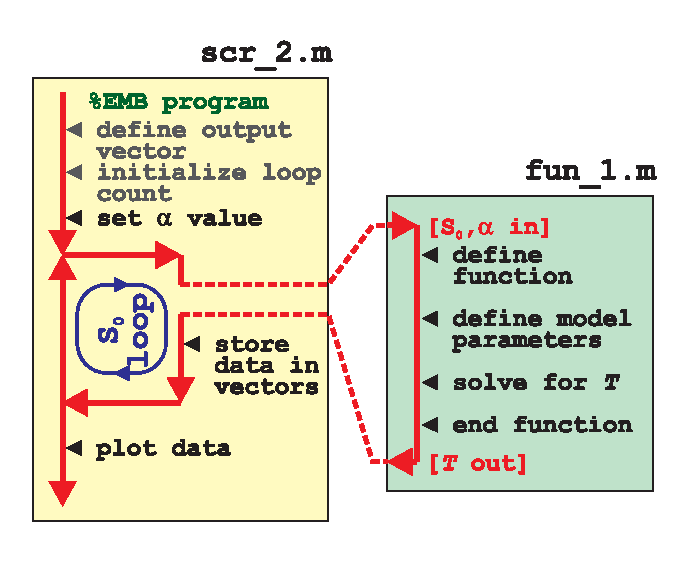
\includegraphics[width=\linewidth]{ch8-schematic-scr2fun1.eps}
\caption{Schematic structure of the model configured to carry out a single parameter sensitivity study.}
\label{fig:ch8-schematic-scr2fun1}
\end{marginfigure}

Pick one of these (i.e. a way of saving a pair of values each time around the loop) and code it up (or better, try all of them in turn!).

Finally, at the end of your program (after the end of the loop), you can now plot (\texttt{plot} or \texttt{scatter}) how \(T\) varies as a function of \(S_{0}\), having saved all the values of \(S\) you tested, plus the corresponding calculated temperatures, in a handy matrix (or pair of vectors).

The structure of your code should look like Figure \ref{fig:ch8-schematic-scr2fun1}. and your resulting figure (depending on the range you assume for \(S\)), something like Figure \ref{fig:ch8-sens1D}.

%------------------------------------------------
%
\newpage

\subsection{Parameter sensitivity experiments using the EBM -- \#2}

In this final sub-subsection, we'll extend the parameter sensitivity analysis of your model to 2D, assuming for instance that you are  now interested in  how \(T\)  varies both as a function of solar constant as well as, as a function of \(\alpha\) (surface albedo). You'll need to vary both \(S\) and \(\alpha\), and in all combinations of the two in order to achieve this. In fact, you'll do this in a grid pattern, with \(S\) increasing in steps on one axis (as before), and \(\alpha\) on the other.

\begin{marginfigure}[-0.5in]
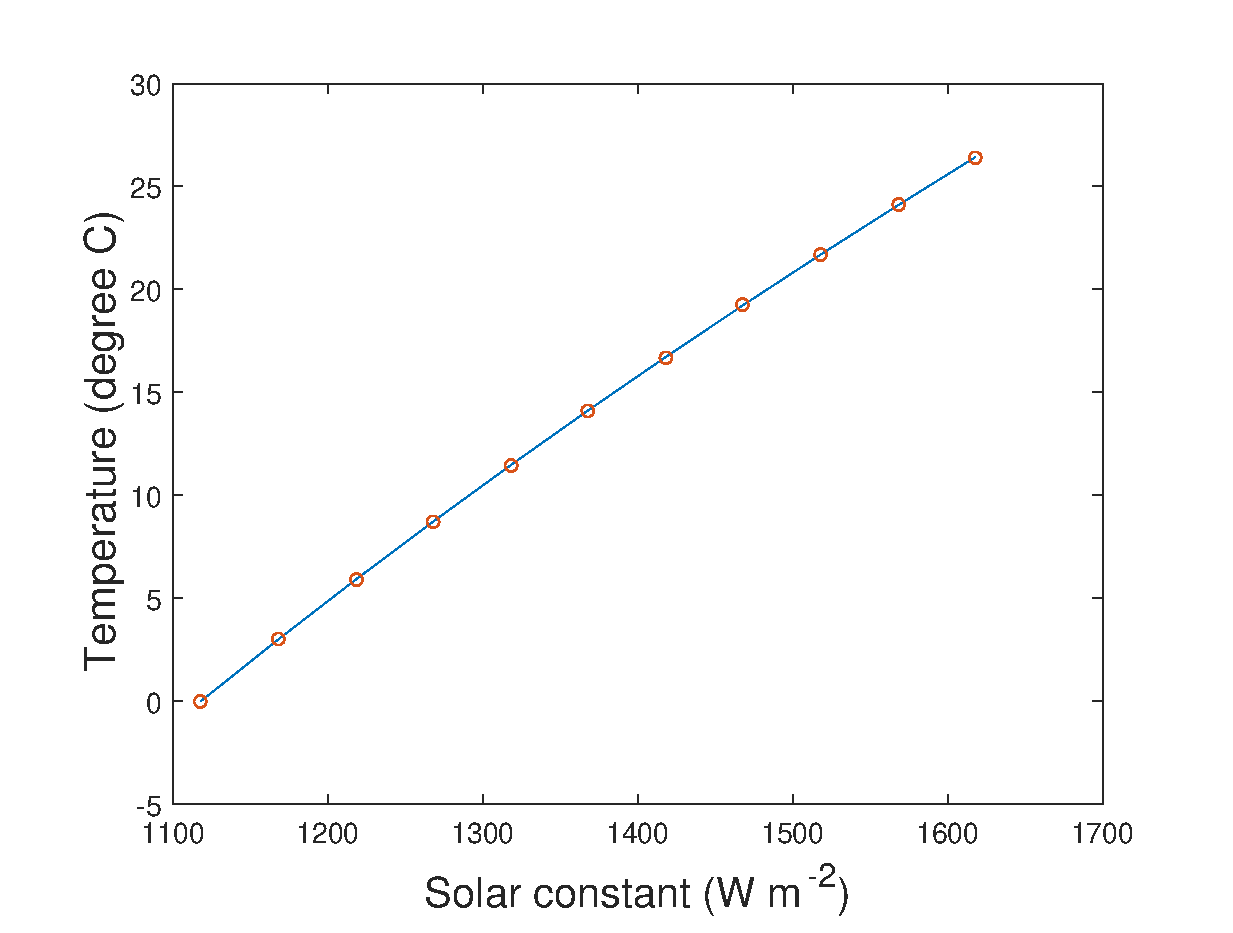
\includegraphics[width=\linewidth]{ch8-sens1D.eps}
\caption{Sensitivity of global mean surface temperature vs. solar constant (mean surface albedo held constant at an albedo value of 0.3).}
\label{fig:ch8-sens1D}
\end{marginfigure}

Hopefully, you might have guessed that you'll need a \textit{nested loop}(?) -- one loop going through all possible values of \(\alpha\), \textit{for each and every possible value of \(S\)}?? i.e. in a structure like:
\vspace{-1mm}\begin{docspec}
\\\textcolor{blue}{for} ...
\\ \ \ \ \textcolor{blue}{for} ...
\\ \ \ \ \ \ \ \textcolor[rgb]{0,0.501961,0}{\% CODE GOES HERE}
\\ \ \ \ \textcolor{blue}{end}
\\\textcolor{blue}{end}
\end{docspec}\vspace{-1mm}

Start with a new (script) \textbf{m-file} ('\texttt{scr\_3}'). For constructing the loop -- you have already seen the 1D example of parameter sensitivity code, and also an example of creating a nested loop for a 2D grid. Chose whether to use counters (e.g. \texttt{n} and \texttt{m}) in the \texttt{for} loops and then derive the values of  \(S\) and \(\alpha\)
from these counters (better), 
 or loop through the values of  \(S\) and \(\alpha\)
directly and create counters (as per for the 1D case).
 Call your \textit{function} (\texttt{fun\_1}) for solving the global surface temperature within the innermost loop (passing it the values of \(S\) and \(\alpha\) generated in the loop). A schematic of the program structure is shown in Figure \ref{fig:ch8-schematic-scr3fun1}.

\begin{marginfigure}[0.0in]
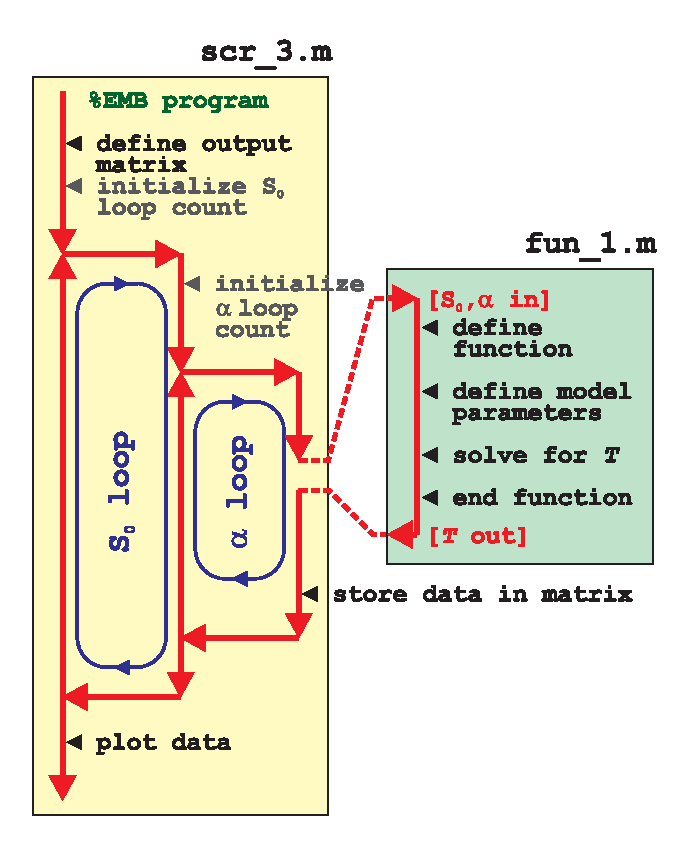
\includegraphics[width=\linewidth]{ch8-schematic-scr3fun1.eps}
\caption{Schematic structure of the model configured to carry out a \uline{double} (in terms of solar constant AND now albedo) parameter sensitivity study.}
\label{fig:ch8-schematic-scr3fun1}
\end{marginfigure}

For saving the data (within the loop), you cannot  simply index the locations you want in a 2D array (matrix) that did not previously exist and expect it to 'grow' as before, because a matrix must have all complete rows and columns and you are generating the results (value of \(T\)), one cell at a time, while you'd need a complete row or column of results in order to append to the results array. Instead, near the start of the code (before the loop), create a matrix of the size of the parameter grid. For example, if you were going to loop through 10 different values of \(S\) and 10 different values of \(\alpha\), you could write:
\begin{docspec}
data\_output = zeros(10);
\end{docspec}
(creating a \(10\times10\) array of zeros). Or if for example, you had 20 different  values of \(S\), and 10 of \(\alpha\):
\begin{docspec}
data\_output = zeros(10,20);
\end{docspec}
(20 columns times 10 rows).

Within an (e.g. \texttt{n,m} loop if you did it that way), you then assign your calculated value of \(T\) to the appropriate location in the array:
\begin{docspec}
\ \ \ \ \ \ data\_output(n,m) = T;
\end{docspec}
Don't forget that you'll also need to know the values of \(S\) and \(\alpha\) that correspond to the column and row numbers. Perhaps save these as 2 individual vector (as per before), or create 2D arrays for them with each element corresponding to an element in the \texttt{data\_output} array, or simply just ignore them for now.

One slight complication if you chose to employ a pair of counters for indexing the results array, and increment their value each time around their respective loops (rather than having a integer count for the loop itself (i.e. \texttt{n} and \texttt{m}) and derive the actual values of  \(S\) and \(\alpha\) from that) -- the innermost counter must be reset in value each time the outer loops starts. This would look like:

\begin{docspec}
count\_outer = 0;
\\\textcolor{blue}{for} ...
\\ \ \ \ count\_outer = count\_outer + 1;
\\ \ \ \ count\_inner = 0;
\\ \ \ \ \textcolor{blue}{for} ...
\\ \ \ \ \ \ \ count\_inner = count\_inner + 1;
\\ \ \ \ \ \ \ \textcolor[rgb]{0,0.501961,0}{\% CODE GOES HERE}
\\ \ \ \ \textcolor{blue}{end}
\\\textcolor{blue}{end}
\end{docspec}

\begin{marginfigure}[-2.0in]
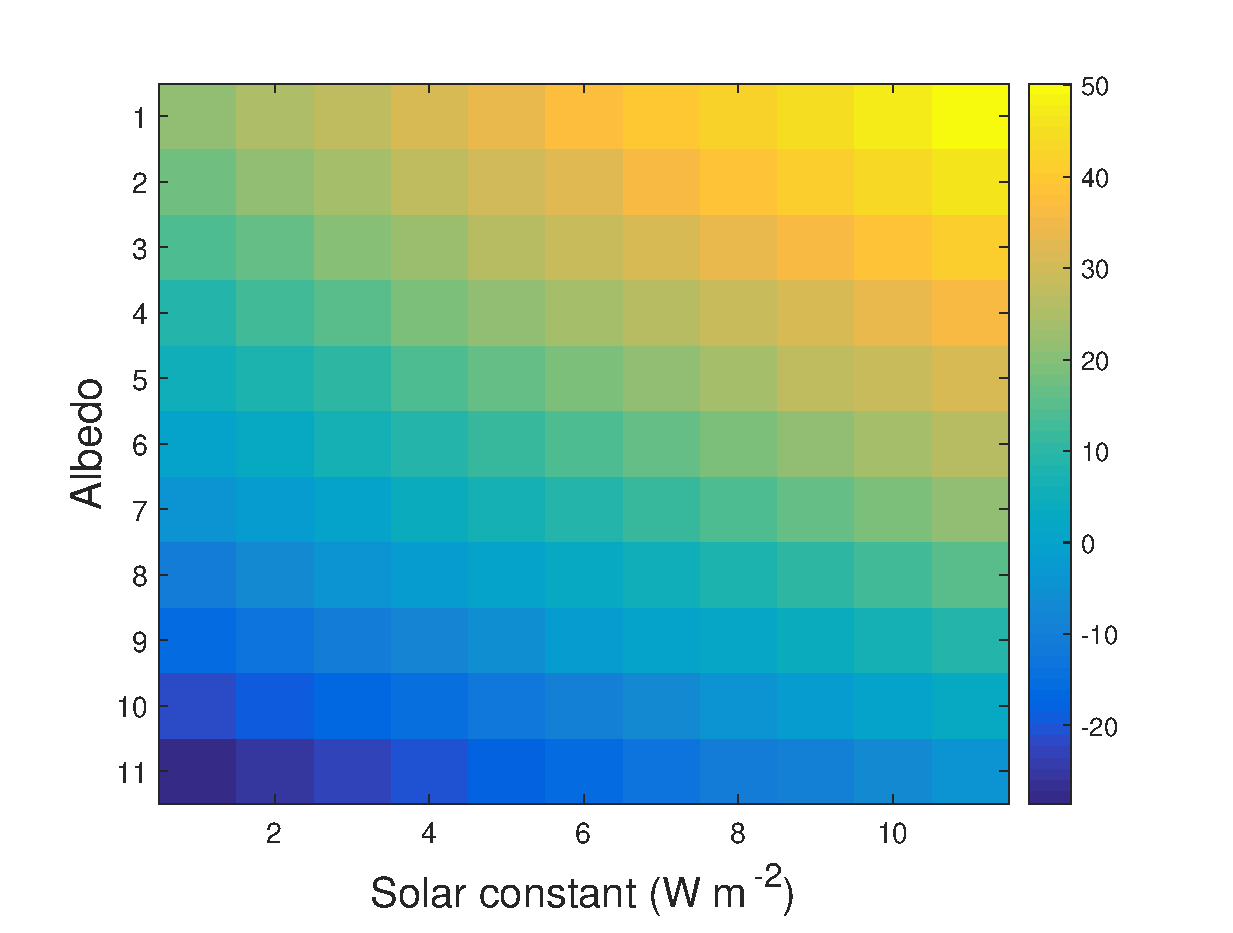
\includegraphics[width=\linewidth]{ch8-sens2D1.eps}
\caption{Global mean surface temperature (\degree C) as a function of solar constant and surface albedo grid point number.}
\label{fig:ch8-sens2D2}
\end{marginfigure}

Be careful here that you increment the value of the count variable \uline{before} using it to index the position in an array -- an index of zero is invalid in \textbf{MATLAB}. Or, you could initialize the count variable to a value of \(1\) before the start of the loop and increment its value \uline{after} you use its value to index a location in the results array.

When you *think* you have this working and have generated a matrix of \(T\) values\sidenote[][-1in]{HINT: create a 2D array of the appropriate size first, before the \textit{loop} starts, using \texttt{zeros}, and then populate it with the values of \(T\) as the \textit{loop} loops.}, plot the resulting surface of \(T\) vs. the two parameters. Rather than using e.g. \texttt{imagesc} (Figure \ref{fig:ch8-sens2D1})\sidenote[][-0.5in]{Note that the temperature grid points are plotted as a function of column and row number and that the plots ends up 'up-side-down' compared to the \texttt{coutourf} version.},  try \texttt{contour}\sidenote[][0.0in]{You'll need to employ \texttt{meshgrid} based on the same 2 vectors of values that the loop creates for \(S_{0}\) and \(\alpha\).} or \texttt{contourf} (e.g. Figure \ref{fig:ch8-sens2D2}).

\begin{marginfigure}[0.0in]
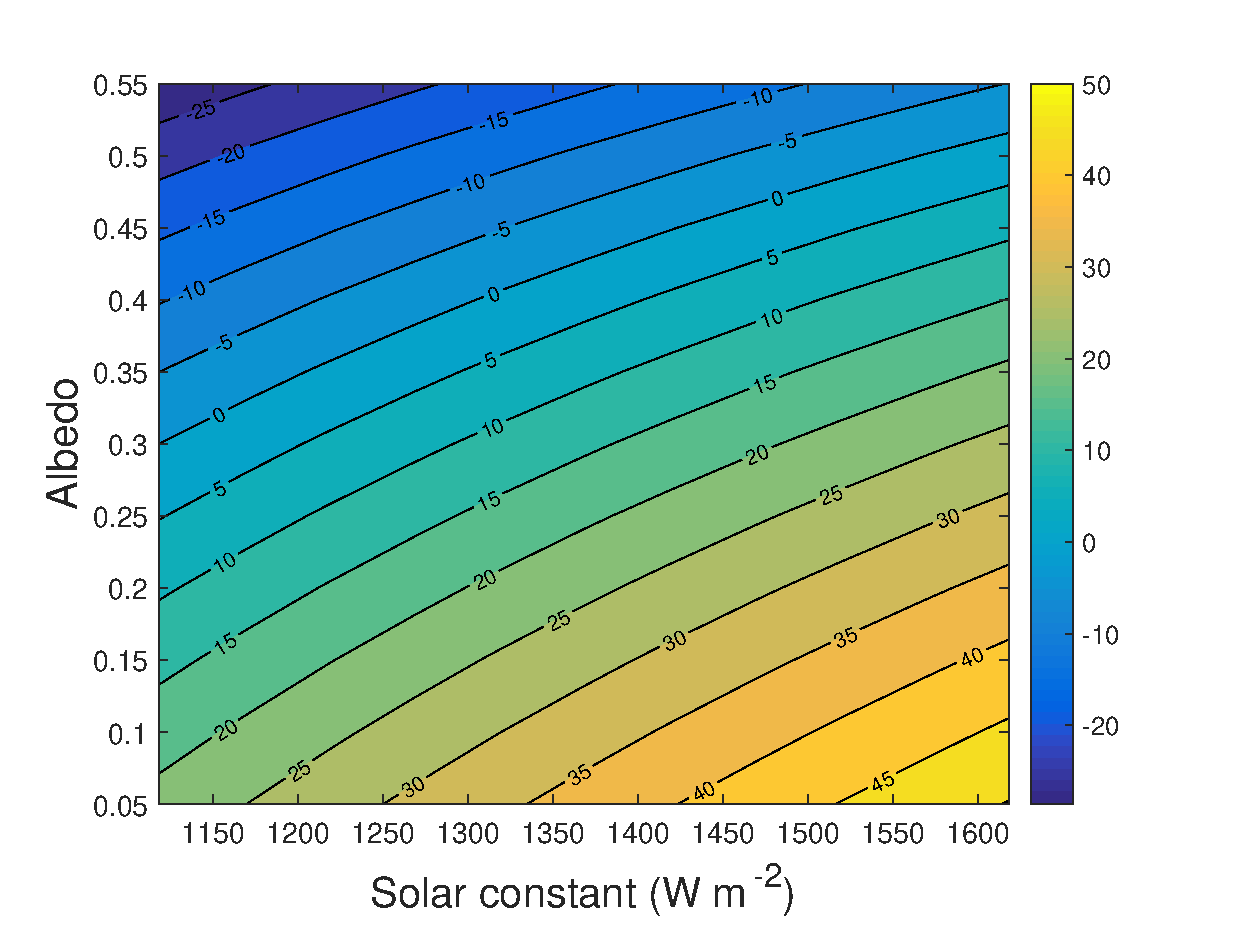
\includegraphics[width=\linewidth]{ch8-sens2D2.eps}
\caption{Global mean surface temperature (\degree C) as a function of the value of solar constant and surface albedo.}
\label{fig:ch8-sens2D1}
\end{marginfigure}

%------------------------------------------------

\newpage

%------------------------------------------------

\section{'Daisy World'}

\begin{marginfigure}[0.5in]
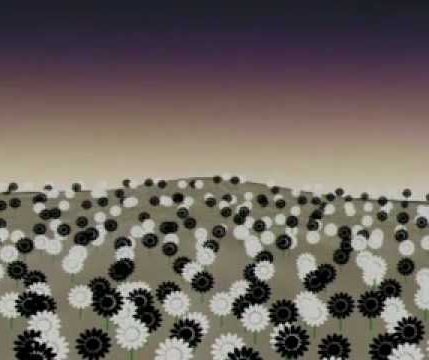
\includegraphics[width=\linewidth]{ch8-daisyworld.png}
\caption{Daisy World}
\label{fig:ch8-daisyworld}
\end{marginfigure}

There is an absolutely classic paper from the early 1980s -- \textit{Watson et al.} [1983] -- that illustrates how simple (biological) feedback on the climate system can lead to a close regulation of global climate over an appreciable span of the Earths past (and future). The premise for this model is a planet covered in bare soil (essentially, as per in the earlier EBM), but on which 2 different species of daisies (could be any pair of plants with contrasting properties) can grow -- one white (high albedo) and one black (low albedo) as per Figure \ref{fig:ch8-daisyworld}\sidenote{As pointed out in \textit{Watson and Lovelock} [1983], the actual 'colors' are immaterial -- just that their albedos differ.}. Because the two species modify their local (temperature) environment and their net growth depends on how close the local temperature is to their optimum growth temperature, a powerful climate feedback operates and as the solar constant increases, the abundance of daisies switches from black to white -- driving an increasing cooling tendency of the planet surface in the face of increasing solar-driven warming. This regulation emerges as a property of the dynamics of the population ecology and interaction with climate and does not require an explicit regulation of climate to be specified. Just dumb daisies doing their day-to-day stuff.

We'll code up this model ... but as before, in discrete stages (aka, the following Subsections).\sidenote{Note that what immediately follows is just a summary list ... not the instructions themselves ...}
\begin{description}[align=right]

\setlength{\itemindent}{-0.2in}

\item [8.2.1] This will be the simplest addition to your previous model\sidenote[][-0.0in]{i.e. the one comprising a loop through time, and within this loop, calls to your function to convert time to solar constant, and take the solar constant (and albedo0 and solve for mean global surface temperature. This was '\# \texttt{scr\_4}' in the previous Section notation.}. You'll create a new 'fixed daisy' function (here called \texttt{fun\_3}) which will take no(!) inputs, and return a value for mean global albedo. You'll also copy-rename yourself a new script ('\texttt{scr\_5}' -- based on your previous \textsf{m-file} \texttt{scr\_4}) and in it, take the albedo value generated by the call to the daisy function, and pass it into your EBM function (\textsf{m-file} \texttt{fun\_1}).

\noindent (See Figure \ref{fig:ch8-schematic-scr5fun1fun2fun3}.)

\item [8.2.2] Now, in the next stage it gets a little more complicated, because in a further new function ('\texttt{fun\_4}' -- copy-renamed-and-edited from \texttt{fun\_3}), you'll modify the equations such that the relative abundance of each daisy type is now responsive to the value of global temperature and incorporates some population dynamics of the daisies.\\ In the main (time since the Sun formed) loop (in \texttt{scr\_5}), the situation thus becomes -- the relative fractions of dark and light colored daisies is now a function of global surface temperature, yet ... global surface temperature, through the mean (fractional area weighted) albedo of the daisies, is a function of the relatively fractions of dark and light colored daisies -- a circularity (feedback loop). We'll resolve this circularity (i.e. come to a steady state solution) by creating an inner loop in \texttt{scr\_5} that comprises only the daisy (abledo) function (\texttt{fun\_4}) and the EBM function and keeps looping until ... well, we'll start by simply prescribing a fixed number of iterations of the loop.

\noindent (See Figure \ref{fig:ch8-schematic-scr6fun1fun2fun4} for a schematic of the code setup.)

\item [8.2.3] Finally (almost) -- we'll allow the daisies affect their *local * (temperature) environment. Now it gets more interesting (honest!). Although the code structure is exactly the same as in the last step\sidenote{A loop through geological time, as per in the previous Section. Within this main loop, you'll have a sub-loop with just the daisy function followed by the EBM function.}, you will require a further copy-rename-and-edit of the previous daisy function ('\texttt{fun\_4}' \(\rightarrow\) '\texttt{fun\_5}') and one further copy-rename-and-edit of the previous script ('\texttt{scr\_6}' \(\rightarrow\) '\texttt{scr\_7}') that calls the daisy function.

\item [8.2.4] In a minor extension to the previous work, we can modify the loop involving  the daisy function and EBM function such that it will proceed until an adequately accurate solution (f0r global temperature) has been converged upon (rather than looping a fixed number of times).  

\end{description}

OK then -- here goes ...

%------------------------------------------------

\subsection{'fixed daisy' daisy-world}

To start: read \textit{Watson and Lovelock} [1983]. You should be able to take away from this some of the essential information that you need to specify and keep track of. For now, we'll just concern ourselves with defining the albedo of bare ground (soil) and the albedo of each daisy together with how much area is covered by each species of daisy.

As summarized above -- create a new function (\texttt{fun\_3}) and configure it so that it returns a single parameter -- albedo. For now it has no inputs.\sidenote[][-2.5in]{A funny sort of function, although pretty well much like \texttt{pi}.} How it relates to your previous program and code for how the Earth's surface temperature evolves over geological time, is illustrated in Figure \ref{fig:ch8-schematic-scr5fun1fun2fun3}.

\begin{marginfigure}[-2.in]
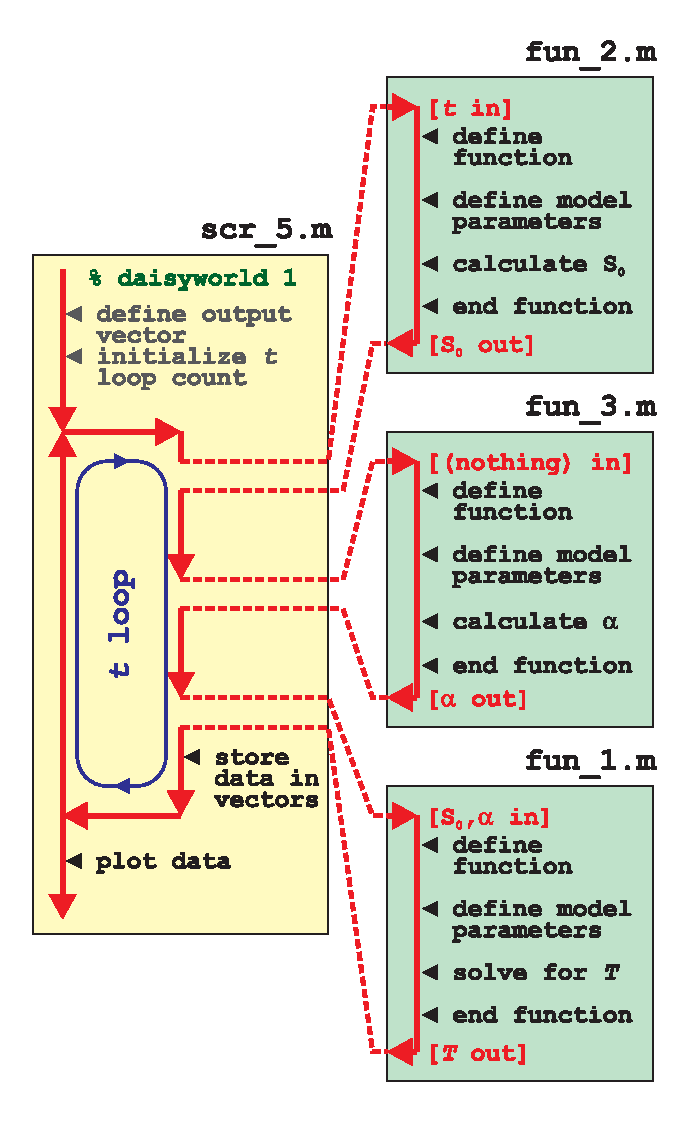
\includegraphics[width=\linewidth]{ch8-schematic-scr5fun1fun2fun3.eps}
\caption{Schematic of the evolution of surface temperature over geological time program, and relationship between main program script, the solar constant and EBM functions, and now the 'daisy' albedo function.}
\label{fig:ch8-schematic-scr5fun1fun2fun3}
\end{marginfigure}

In the daisy/albedo function (\texttt{fun\_3})  near the top, define yourself some parameters for the daisy model:
\begin{docspec}
\% define model parameters -- daisy albedo
\\par\_a\_s = 0.3; \% albedo -- bare soil
\\par\_a\_b = 0.1; \% albedo -- black daisies
\\par\_a\_w = 0.5; \% albedo -- white daisies
\\\% define model parameters -- daisy land fraction
\\fb = 0.01; \% (land) fraction -- black daisies
\\fw = 0.01; \% (land) fraction -- white daisies
\end{docspec}
(or using whatever parameter names you prefer). Here, the albedo values associated with each daisy type are fixed and will be used regardless of what the model does. The values have been chosen, assuming equal proportions of black and white daisies, to given an average of 0.3 -- the albedo of bare soil and also the assumed value in the previous EBM. You'll modify and play with this value all too soon enough. The surface area fraction values are just initial values to start the model off with.\sidenote[][-0.0in]{As you'll come to see subsequently, these cannot be zero. Or rather, a daisy species can start with a fractional area of zero, but you'll never ever get any of that species growing, regardless of the environmental conditions (because there are none to start with!).}

These parameters relate to the symbols in the equations that follow, as follows:

\begin{itemize}[noitemsep]
\setlength{\itemindent}{.2in}
\item[\(\alpha_{s}\)] -- \texttt{par\_a\_s} (albedo -- bare soil)
\item[\(\alpha_{b}\)] -- \texttt{par\_a\_b} (albedo -- black daisies)
\item[\(\alpha_{w}\)] -- \texttt{par\_a\_w} (albedo -- white daisies)
\item[\(F_{b}\)] -- \texttt{fb} (land) fraction -- black daisies
\item[\(F_{w}\)] -- \texttt{fw} (land) fraction -- white daisies
\end{itemize}
\vspace{0mm}

Next, and actually the only line of any note in the function -- you need to calculate the average albedo\sidenote[][-0.5in]{Note that it is very easy to accidently prescribe a total area covered by daisies of >100\%. You should ideally put a check (\texttt{if ... end}) in the code before it tries to calculate anything for whether the total area initially covered by daisies exceeds what is possible. If this is the case, your code might spit out a warning message (a simple \texttt{disp} command would do). You might also terminate your program (see \docenv{exit}).} -- calculated based on the area weighted average of: bare soil, white daisies, black daisies. The calculation is simple and you already have the areas of the two species of daisy as fractions. You weight the contribution to global albedo by the albedo of each daisy by its fractional area. You then just need to calculate the fraction of the Earths surface that is bare soil -- the area fraction not covered by daisies. In maths-speak, the mean albedo is given by:
\begin{docspeclarge}
\(\alpha = F_{w}\cdot\alpha_{w} + F_{b}\cdot\alpha_{b} + (1.0-F_{w}-F_{b})\cdot\alpha_{s}\)
\end{docspeclarge}
where \(\alpha_{w}\), \(\alpha_{b}\), and \(\alpha_{s}\), \(F_{w}\), and \(F_{b}\) are as defined above. Bare soil is simply whatever the fraction of the planet is not covered by daisies, i.e. \((1.0-F_{w}-F_{b})\). 

You simply need to translate all this into \textbf{MATLAB} code using the parameters you defined earlier (for  \(\alpha_{w}\), \(\alpha_{b}\), and \(\alpha_{s}\), and  \(F_{w}\) and \(F_{b}\)). The code will look pretty well much like the equation, but you substituting whatever variable/parameter names you have chosen for the symbols in the maths:
\begin{docspec}
\textcolor[rgb]{0,0.501961,0}{\% calculate mean albedo\\}
albedo = Fw*par\_a\_w + Fb*par\_a\_b + (1.0 - Fw - Fb)*par\_a\_s;
\end{docspec}
To be neater, we could also pre-calculate the fraction of bare ground, \(F_{g}\), and make ourselves a slightly shorter (and easier-to-debug) mean albedo calculation, e.g.
\begin{docspec}
\textcolor[rgb]{0,0.501961,0}{\% calculate fractional area of bar ground\\}
Fg = (1.0 - Fw - Fb);\\
\textcolor[rgb]{0,0.501961,0}{\% calculate mean albedo\\}
albedo = Fw*par\_a\_w + Fb*par\_a\_b + Fg*par\_a\_s;
\end{docspec}

Add these lines of code, which will be the one and only calculation that this particular \textbf{MATLAB} \textit{function} ((\textsf{fun\_3}), Figure \ref{fig:ch8-schematic-scr5fun1fun2fun3}) carries out, just before the \texttt{\textcolor{blue}{end}} of the function.

\begin{marginfigure}[-2.0in]
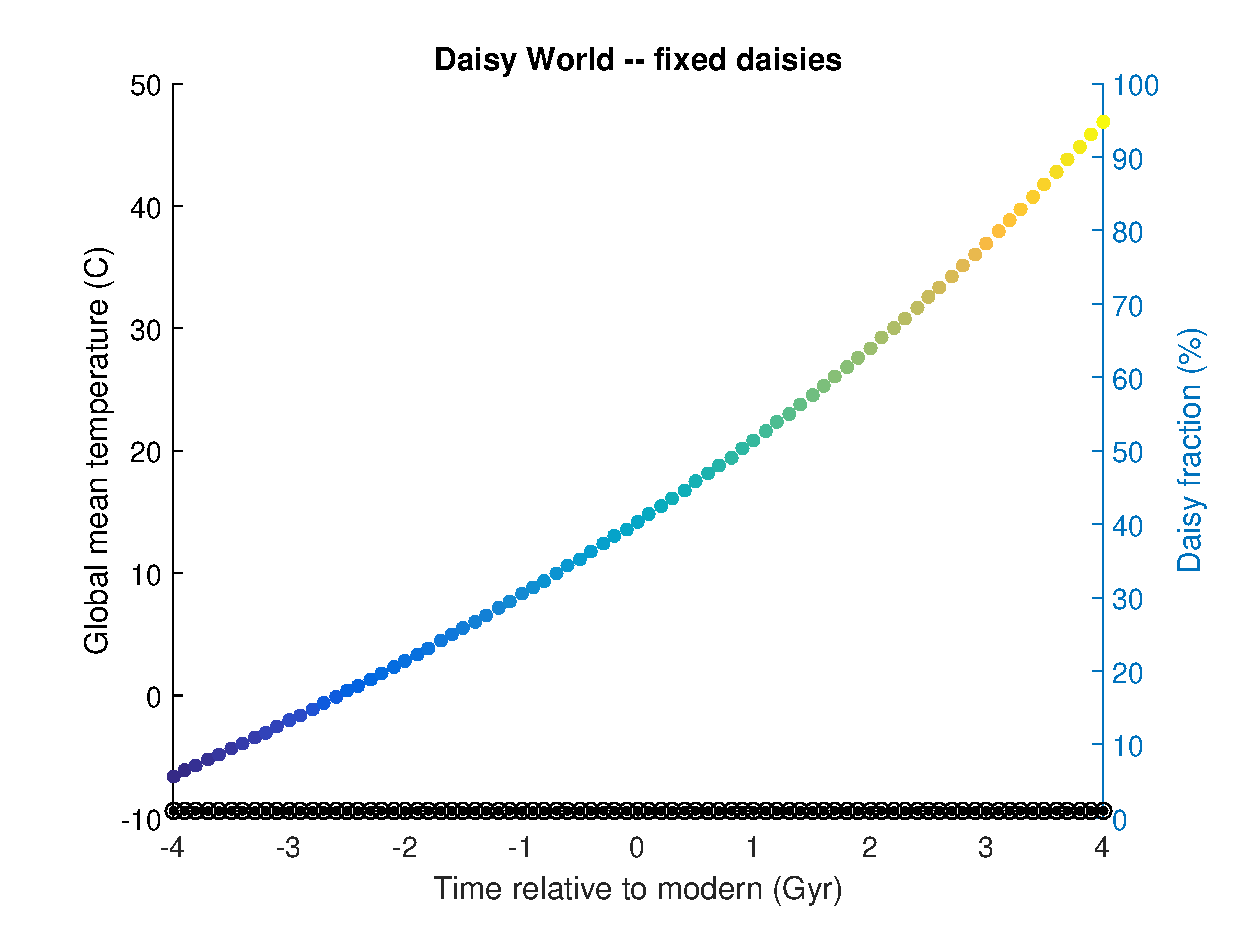
\includegraphics[width=\linewidth]{ch8-daisy1.eps}
\caption{Evolution of global surface temperature and the two populations of daisies with time ... but with no change allowed in the daisy populations (d'uh!). The fractional coverage of white daisies is shown by large empty circles, and for black, by small filled black circles. Data points for mean surface temperature are color-coded by temperature (color scale not shown).}
\label{fig:ch8-daisy1}
\end{marginfigure}

That is actually it. All the variable/parameter values are specified and fixed in the daisy function (see above), so nothing particularly exciting is going to happen ... Regardless -- run the the complete model with the value of albedo now depending on the fraction of white and black daisies  -- it should look identical to before in terms of the evolution of surface temperature with time (it must, because the default parameters above ensure that the mean albedo is always 0.3 and the daisies don't even know anything about growing (or dying) yet). Model (surface temperature) output, including how the populations of the 2 species of daisy also vary with time, is shown in Figure \ref{fig:ch8-daisy1}).

You might play briefly with the prescribed daisy area fractions (\texttt{Fb} and \texttt{Fw}) and albedo values (\texttt{par\_a\_b} and \texttt{par\_a\_w}) and e.g. check that when you specify a configuration with 100\% of land area covered by black daisies, the climate is much warmer throughout the simulation, and when white daisies are assigned an initial value of 1.0, the climate is always much cooler compared to in the default simulation.

%------------------------------------------------

\subsection{'dumb daisy' daisy-world}

\vspace{-2mm}
\newthought{Step \#2} in the evolution of the Daisy World model, and for a modification which will actually make something 'happen' (i.e. the simulation will be different to that of the default EBM based simulation of mean global temperature response to increasing \(S_{0}\)). The daisy population is now going to grow and die (but unlike Southern California, not burn), with their relative fractions  changing over time until an equilibrium is reached (for a particular specified value of \(S_{0}\)).
\textit{Watson and Lovelock} [1983] give a simple population model formulation for the change in area fraction covered by both sorts of daisy with time (also see Box) that we will implement here.

\marginnote[-3.75in]{\begin{mdframed}[backgroundcolor=light-blue, roundcorner=10pt,leftmargin=1, rightmargin=1, innerleftmargin=5, innerrightmargin=5, innertopmargin=5,innerbottommargin=5, outerlinewidth=1, linecolor=light-gray]
\textbf{Daisy population dynamics (1)}
\\For an area fraction occupied by white and black daisies of \(F_{w}\) and \(F_{b}\), respectively, the change in occupied fractional area with time (\(t\)) can be written:
\begin{docspec}
\(dF_{w}/dt = F_{w}\cdot(x\cdot\beta_{w}-\gamma)\)
\\\(dF_{b}/dt = F_{b}\cdot(x\cdot\beta_{b}-\gamma)\)
\end{docspec}
where \(x\) is the free (i.e. not occupied by daisies of any color) area of (fertile) ground, equal to:
\begin{docspec}
\(x=1.0-F_{w}-F_{b}\)
\end{docspec}
(assuming here, unlike the more general case in \textit{Watson and Lovelock} [1983], that all the land area is potentially fertile), \(\beta\) is a temperature-dependent growth function (one for each species of daisy), and \(\gamma\) the mortality rate (as a proportion of the area covered by that species of daisy per unit time). The value of \(\gamma\) given in  \textit{Watson and Lovelock} [1983] is 0.3, but this could be a parameter that you could play about with and investigate its effects.
\\To simplify things to start with, growth is a function only of the global mean temperature (in \degree C):
\begin{docspecmargin}
\(\beta_{w} = 1.0-0.003265\cdot(22.5-T)^{2}\)
\\\(\beta_{b} = 1.0-0.003265\cdot(22.5-T)^{2}\)
\end{docspecmargin}
(where the value of \(22.5\) \degree C is a reference temperature and represents where optimal (maximum) growth occurs).
\end{mdframed}}

The unit of population in Daisy World is fractional area covered (rather than an absolute number of individuals as we had before, but these are pretty much completely interchangeable). So from generation-to-generation (or on each subsequent time step, if you prefer to think of it that way), the fractional area of each species will grow or shrink, depending on whether mortality is higher than growth. Both growth and mortality are formulated as being dependent on the fractional area (at the previous time-step), i.e. growth in covered area depends on how much is already covered.\sidenote{Note the parallels with before -- the new fractional area is dependent on the previous area, whereas before it was the new population size (number of individuals) that was dependent on the previous population size.)} Similarly, mortality also depends on the current areas of daisies. The growth rate is further modified by the available fractional area, such that as the area left shrinks, the growth rate shrinks. (Effectively, this is perhaps trying to account perhaps for shrinking resources available for further growth. It also has the effect of adding numerical stability to the model and helps presents over-shoots where the total fractional area covered by daisies far exceeds 1.0 ...). 
?

How then to implement changing areas and growth of daisies in code? (We'll come to how to translate the equations into code after ensuring we have the basic structure of the program built. A general programming Plan of Action is given in the margin.)

Figure \ref{fig:ch8-schematic-scr6fun1fun2fun4} gives a schematic of the overall code structure for this model. The new difficulty here is that the relative fractions of dark and light colored daisies is a function of global surface temperature, yet ... global surface temperature, through the mean (fractional area weighted) albedo of the daisies, is a function of the relatively fractions of dark and light colored daisies -- a circularity (feedback loop). We resolve this circularity (i.e. come to a steady state solution) by creating an inner (nested) loop that comprises only the daisy function and EBM function.

\textbf{\textcolor{red}{DON'T PANIC.}} There are actually only 2 (or 3-ish), relatively incremental changes, compared to previously. Start off by noting what is the same -- both the function for calculating the solar constant as a function of time (\texttt{fun\_2}) and the EBM model (\texttt{fun\_1}) (temperature as a function of solar constant and albedo) are exactly the same as before. The loop in (geologic time) and hence some of the script (\texttt{scr\_6}) is also the same. What is different and yet to-do?

\marginnote[-4.0in]{
Programming strategy:
\begin{itemize}[noitemsep]
\setlength{\itemindent}{.2in}
\item In general -- start by identifying any constants -- i.e. fixed and invariant, fundamental values, such as \(\pi\) or the Stefan-boltzmann constant. These values could be hard-coded into the equation as numbers, but better is to replace them with variables that you'd define at the top of the m-file as this makes for neater and easier-to read \textbf{MATLAB} code.
\item Next identify any parameters -- values that are not fundamental properties of the universe, but may be considered invariant for sequential uses of the equation. The characteristic albedos of the two species of daisies is a good example -- these values are 'fixed', although, one day you might change them. If the code file is a script -- define \textbf{MATLAB} variables and assign values to them, near the start of the code file. Otherwise, if a function, you may need to pass these parameters into the function and so they need to appear in the function definition on the 1st line of the code.
\item Identify any output variables, i.e. result(s) of the calculation. In a function, these are invariably pass back out and hence need to appear in the function definition on the 1st line of the code. Output variable may also be input variables -- i.e. a calculation may take the current value of a variable (as an input), update it, and then pass it back out. In which case, the variable will need ot appear as both input and output. Perhaps pick distinction variable names to avoid confusion, e.g. \texttt{var\_in} and \texttt{var\_out}. 
\item You may have local variables (i.e. used only within the script and out outside of it). If scalars, these need not be defined and initialized, unless used as e.g. a counting or running-sum variable. If in doubt, maybe also define and initialize e.g. to zero local variables.
\item Otherwise, it is mostly just a case of writing the maths, in \textbf{MATLAB} -- changing symbols where necessary and replacing the letters (invariably) used in the equations with your variable names.
\end{itemize}
}

\begin{enumerate}
\setlength{\itemindent}{.2in}

\item Lets start with the daisy (albedo) function (which will be based on the previous, \texttt{fun\_3} one). You could deal with the inputs and outputs first. As as well as \(T\), the previous values of the fractional areas of the two daisies (\(F_{w}\), \(F_{b}\)) are also required by the function (which is different from before where the values were assumed and the respective parameters set at the start of the function\sidenote{So if you are copy-pasting the previous Daisy function, you need to delete the lines: 
\begin{docspecmargin}
par\_f\_w = 0.01;
\\par\_f\_b = 0.01;
\end{docspecmargin}}).  This is because each time the daisy fractional area function is called, the fractional areas are updated (hence why they are inputs). And outputs. Because the daisy function is updating the fractional areas, these two parameters also need to be outputs too.
So the very first thing to do is to modify the function definition, re-saving it as \texttt{fun\_4} (see Figure \ref{fig:ch8-schematic-scr6fun1fun2fun4}), so that the inputs are:
\begin{docspec}
\(T, F_{w}, F_{b}\)
\end{docspec}
and the outputs are:
\begin{docspec}
\(\alpha, F_{w}, F_{b}\)
\end{docspec}
(see help of various sorts on \textit{functions}, but it not at all a fundamental change as to compared to before). Of course, you need to substitute the maths symbols for the actual variable and parameter names you choose to use.
\\Then, the only other development in the function, is to implement the equations for daisy growth/death (see Box) and update the values of \(F_{w}, F_{b}\).

\begin{marginfigure}[-0.0in]
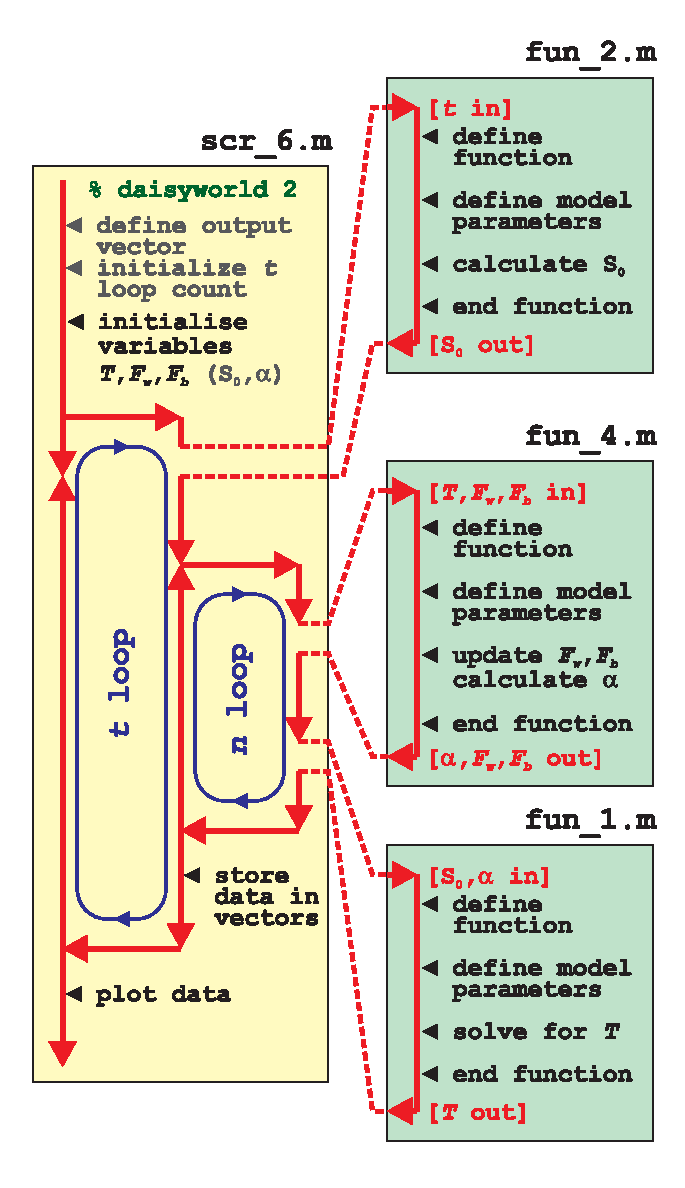
\includegraphics[width=\linewidth]{ch8-schematic-scr6fun1fun2fun4.eps}
\caption{Schematic of the evolution of surface temperature over geological time program, and relationship between main program script, the solar constant, EBM, and 'daisy' albedo functions. Note the creation of an inner loop, with EBM, and 'daisy' albedo functions called from within this, while the solar constant remains called form the start of the outer loop as before.}
\label{fig:ch8-schematic-scr6fun1fun2fun4}
\end{marginfigure}

\item How to translate the given daisy population/growth equations into code? We could start by substituting the value of \(\gamma\) for its literature value of \(0.3\) to make it a little less scary. And also set the growth rate function, \(\beta\) to \(1.0\) for now, so that does not distract us either. The now simpler equations look like:
\begin{docspec}
\(dF_{w}/dt = F_{w}\cdot(x-0.3)\)
\\\(dF_{b}/dt = F_{b}\cdot(x-0.3)\)
\end{docspec}
which says that the change in fractional area (\(dF\)), from one iteration (generation or time step) to the next is proportional to the current fractional area (\(F\)) multiplied by some stuff (\(x-0.3\)).

We could re-write this in terms of a (loop) iteration number (\(n\)) and also ignoring for now which daisy (black or white) we are talking about:
\begin{docspec}
\(F_{(n+1)}=F_{(n)} + F_{(n)}\cdot (x-0.3)\)
\end{docspec}
or rearranging:
\begin{docspec}
\(F_{(n+1)}=(1.0 + x-0.3)\cdot F_{(n)}\)
\end{docspec}
which says quite simply that the next fractional area estimate, is equal to the current one, multiplied by \((1.0 + x-0.3)\). This should look pretty familiar to you now and you should know how to code this up, e.g.
\begin{docspec}
\textcolor{blue}{for} n=1:100\\
\ \ \ F = (1.0 + x - 0.3)*F;\\
\textcolor{blue}{end}
\end{docspec}
taking \(100\) loop iterations as an example. But ... we are not writing the population  and albedo update code directly in the loop, but rather, it is going into \textsf{fun\_4} and the function is called from within the \texttt{\textcolor{blue}{for} n=1:100 ...} loop (Figure \ref{fig:ch8-schematic-scr6fun1fun2fun4}).
 So rather (schematically):
\begin{docspec}
\textcolor{blue}{for} n=1:100\\
\ \ \ fun\_2()\\
\ \ \ fun\_4()\\
\ \ \ fun\_1()\\
\textcolor{blue}{end}
\end{docspec}
and within the function:
\begin{docspec}
F = (1.0 + x - 0.3)*F;
\end{docspec}
 
The value of \(x\) in the equation is simply the fraction of the planet not covered in daisies. And if we also bring both daisies and their respective fractional areas back into the picture:
\begin{docspec}
x = 1.0 - Fb - Fw;\\
Fb = (1.0 + x - 0.3)*Fb;\\
Fw = (1.0 + x - 0.3)*Fw;\\
\end{docspec}

\item Now you are in a position to worry about the temperature dependent functions for growth, which were:
\begin{docspec}
\(\beta_{w} = 1.0-0.003265\cdot(22.5-T)^{2}\)
\\\(\beta_{b} = 1.0-0.003265\cdot(22.5-T)^{2}\)
\end{docspec}

These are actually pretty simple -- you take temperature, subtract it from a value of \(22.5\) and square it, multiply it by \(0.003265\) and subtract from \(1.0\) ...
\begin{docspec}
bb = 1.0 - 0.003265*(22.5-T)\(^{\wedge}\)2\\
bw = 1.0 - 0.003265*(22.5-T)\(^{\wedge}\)2
\end{docspec}
Really -- just as it looks written down mathematically. So now the content of \textsf{fun\_4} will contain:
\begin{docspec}
x = 1.0 - Fb - Fw;\\
bb = 1.0 - 0.003265*(22.5-T)\(^{\wedge}\)2\\
bw = 1.0 - 0.003265*(22.5-T)\(^{\wedge}\)2\\
Fb = (1.0 + x*bb - 0.3)*Fb;\\
Fw = (1.0 + x*bw - 0.3)*Fw;
\end{docspec}

\item So far, in \textsf{fun\_4} you have updated the  area fraction remaining (bare ground), updated the growth factors for the two species of daisy, and then updated the fractional areas of both species of daisy. Remaining, in this function, is to take the new fractional areas, and update the mean albedo (which is then returned from the function as an output):
\begin{docspec}
\textcolor[rgb]{0,0.501961,0}{\% update mean albedo\\}
albedo = x*par\_a\_s + Fw*par\_a\_w + Fw*par\_a\_b;
\end{docspec}

After this function returns the new updated values of mean albedo (and the two fractional daisy areas in case we want them for plotting later), the EBM function (\textsf{fun\_1}) is called (in the inner loop) (Figure \ref{fig:ch8-schematic-scr6fun1fun2fun4}).

\item Lastly, the initialization of the main program (\texttt{scr\_6}) will be a little different from before. Because the daisy function now takes as input, \(F_{w}\) and \(F_{b}\) -- you'll need to give these variables each an initial value (near the start of the program) so that first time the function is called, there is a value for the equations to work with. Similarly, temperature \(T\) now also becomes an input to the daisy function (and it is not set anywhere else beforehand in the very first iteration of the loops), so it also needs an initial value to be assigned.\sidenote[][-2.5in]{For completeness, you could also initialize \(S_{0}\) and \(\alpha\), but it is not strictly needed, as they are calculated and defined before they are first used.}

\end{enumerate}

\begin{marginfigure}[-1.5in]
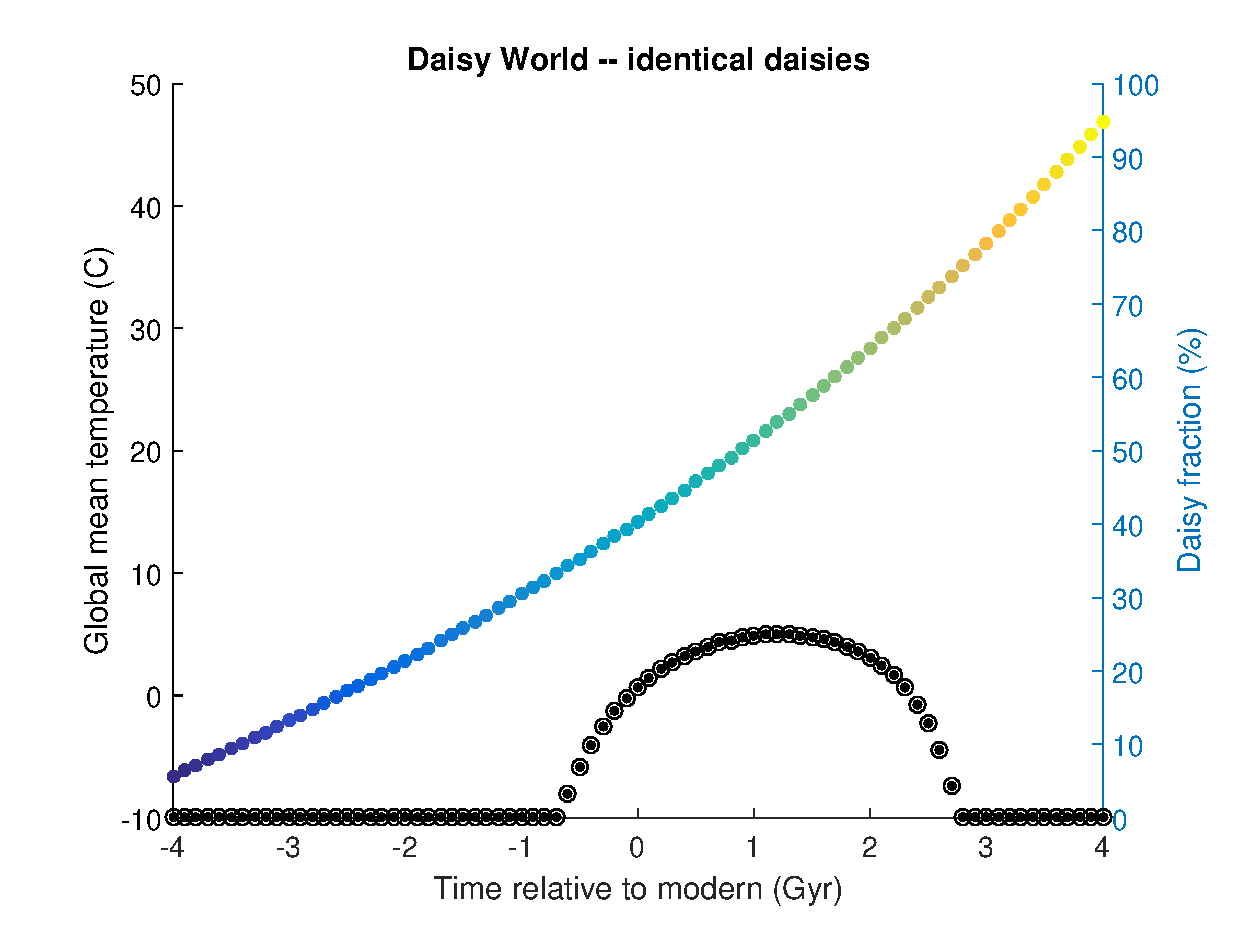
\includegraphics[width=\linewidth]{ch4-daisy-model2.eps}
\caption{Evolution of global surface temperature and the two populations of daisies with time ... but now assuming that the growth of each depends on the global mean surface temperature.}
\label{fig:ch4-daisy-model2}
\end{marginfigure}

If you have set this daisy population dynamics enabled EBM (a DPDE-EBM!) up correctly, and drive it with your -4.0 to +4.0 Ga solar constant calculating script, you should get something like Figure \ref{fig:ch4-daisy-model2}.

OK, so actually, this is not different in terms of the global mean temperature response (to solar evolution), to before. But then again, you have set both species of daisy with the same temperature growth response. In other words, as the white daisies with a high albedo grow, so to the black ones with a low albedo. Equally. And their different albedos balance, meaning that \(\alpha\) still never changes. One thing you could try to liven things up a little is to change on of the value of \(\beta\) (and/or \(\gamma\)) so that their population dynamics are not identical. Now, if the relative abundance of white and black daisies changes, so too with global mean albedo and hence global temperature.

%------------------------------------------------

\subsection{'clever daisy' daisy-world}

The last step is to give each species of daisy a different environmental preference for growth (why? because that is how the World works -- different plants and ecosystems tend to inhabit different environmental regimes as a result of being (evolutionary) adapted to different environmental parameters). \textit{Watson and Lovelock} [1983] assume that both species of daisy have the same temperature preference but modify their local environment differently -- white daisies inducing a local cooling relative to the global mean temperature, and the presence of black daisies driving a local heating (see Box). The result is Figure \ref{fig:ch4-daisy-model3}.

\marginnote[-2.0in]{\begin{mdframed}[backgroundcolor=light-blue, roundcorner=10pt,leftmargin=1, rightmargin=1, innerleftmargin=5, innerrightmargin=5, innertopmargin=5,innerbottommargin=5, outerlinewidth=1, linecolor=light-gray]
\textbf{Daisy population dynamics (2)}
\\To make the different species of daisies interact differently with the environment, the temperature-dependent modifiers of growth are made functions of the local (to the daisy population or individual), rather than global, temperature:
\begin{docspecmargin}
\(\beta_{w} = \\ 
1.0-0.003265\cdot(22.5-T_{w})^{2}\)
\\\(\beta_{b} = \\
1.0-0.003265\cdot(22.5-T_{b})^{2}\)
\end{docspecmargin}
There are all sorts of says of defining how the local temperature deviates form the global mean. In \textit{Watson and Lovelock} [1983] this is simply reduced to a simple deviation that scales linearly with the difference between mean global and local (daisy) albedo:
\begin{docspecmargin}
\(T_{w} = T+q\cdot(A-A_{w})\)
\\\(T_{b} = T+q\cdot(A-A_{b})\)
\end{docspecmargin}
(noting that A is mean planetary albedo here, not alpha as was the case in the original (non daisy enabled) EBM, while \(A_{b}\) and \(A_{w}\) are the albedos of black and white daisies, respectively).
\\\(q\) is a simple scaling factor that describes how strongly the local temperature deviates from the mean (or conversely, how efficiently heat energy is mixed between differen daisy fractions) and is assigned a default value of 10.0. 
\end{mdframed}}

In the code -- first copy \texttt{fun\_4} \(\rightarrow\) \texttt{fun\_5}, and \texttt{scr\_6} \(\rightarrow\) \texttt{scr\_7}, remembering to now call \texttt{fun\_5} from within the inner loop in \texttt{scr\_7}. (Otherwise, the structure of the model is the same as before.)
 
In \texttt{fun\_5}, modify the equations of the growth factor \(\beta\) for each species of daisy as per the equations in the Box. Now, instead of using \(T\) (the global mean temperature) in both growth equations, each equation has its own local temperature -- one associated with black daisies (\(T_{b}\)) and one with white (\(T_{w}\)). The local temperatures are calculated as deviations from the global mean, as per the equations in the Box. You'll need to calculate \(T_{b}\) and \(T_{w}\) in the code first, before calculating the values of \(\beta\).

Now the behaviour of the system and the evolution of global mean surface temperature with time, is very different. Towards the start of the experiment, and at very low values of \(S_{0}\), the global mean temperature is too cold to support a daisy population (of either type). As the value of \(S_{0}\) increases, initially global mean temperature follows the path it did before, in the absence of daisies (or with fixed, or equal populations). At a certain point, black daisies, because of their advantage that they absorb more sunlight and drive a locally warmed climate, take off in population and rise to dominate ~70\% of the land surface. The global mean temperature transitions sharply to a much higher temperature state. As \(S_{0}\) further increases in value, they increase slightly further in dominance (and global temperature climb a little further in response) until locally they reach their optimal temperature for growth. Past this (optimal temperature) point, white daisies start to grow and slowly replace the black ones. Global climate is almost perfectly stabilized during this interval. Beyond this, there is a short interval where black daisies die out and white daisies go on to reach their own (local) temperature optimum. Beyond this again, everything suddenly goes extinct in a rapid warming feedback of increasing temperatures, declining white daisy numbers, further solar radiation absorption and warming, etc etc. How everything is dead and I how you are feeling happy with yourself.

\begin{marginfigure}[0.0in]
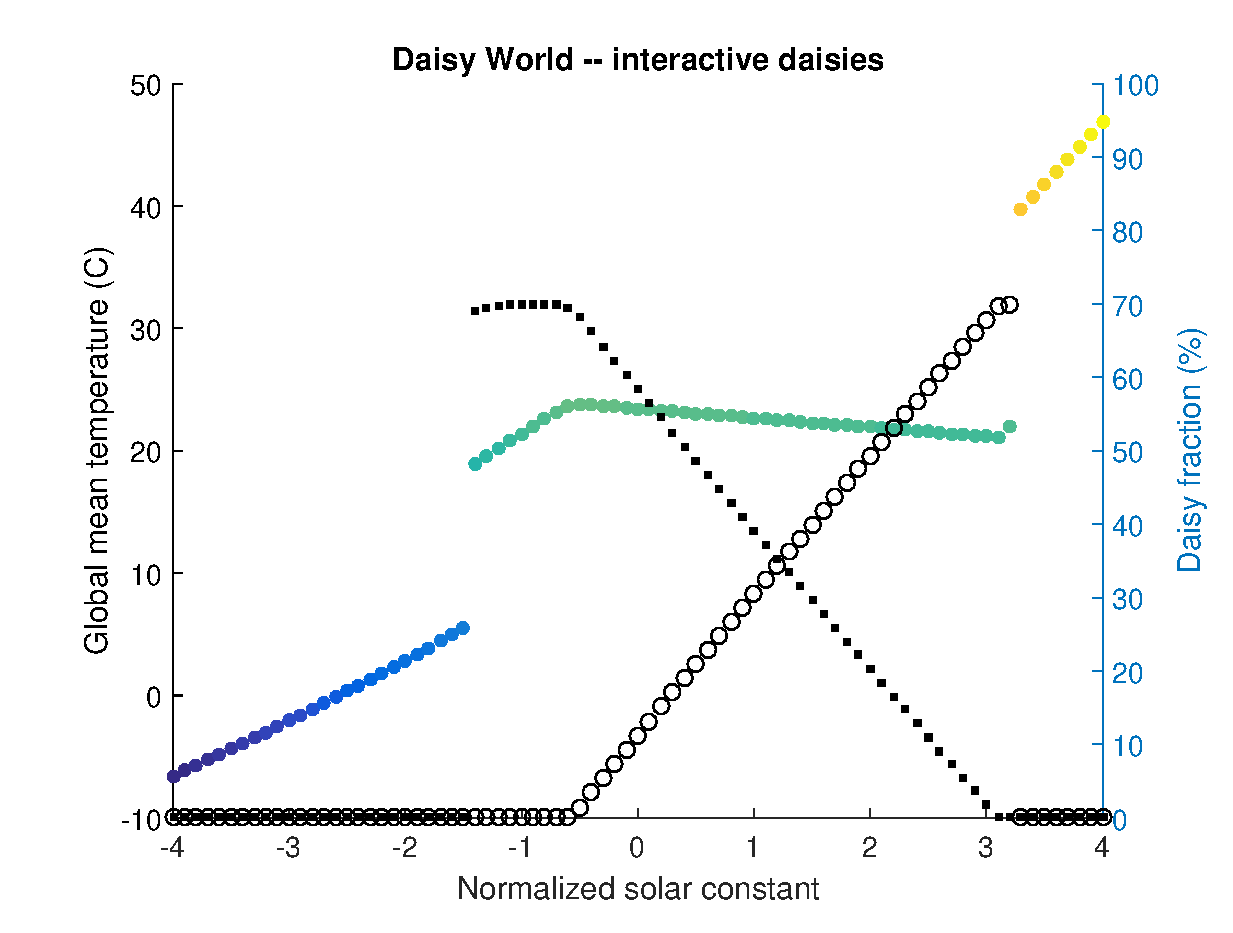
\includegraphics[width=\linewidth]{ch4-daisy-model3.eps}
\caption{Evolution of global surface temperature and the two populations of daisies with time.}
\label{fig:ch4-daisy-model3}
\end{marginfigure}

You could code this modification in -- adjusting the (local) value of \(T\) that each species of daisy 'sees' (as per the Box and the reference). Or ... we could simply give them different temperature optima, which is what the value of 22.5\degree C accomplishes in the temperature-dependent growth modifier equation. For now, this is the way-simpler approach and involves only a minimal edit to your existing daisy function. So where in the equation for \(\beta_{w}\) and \(\beta_{b}\) you currently have values of \(22.5\) (\degree  C) in each -- try making these different. Reasonable would be to assume that the white daisies are more adapted to hot climates and hence have a higher temperature tolerance, with black daisies being better adapted to colder climates, using their higher albedo and presumably local heating to make up for a colder ambient environment. (You could be able to come up with something not entirely dissimilar to Figure \ref{fig:ch4-daisy-model3}.)

%------------------------------------------------

\subsection{Efficient and 'clever daisy' daisy-world}

The purpose of the inner loop is to calculate the equilibrium planetary temperature for each value of \(S_{0}\). It may be that an equilibrium is reached much sooner than the \(100\) loop iterations that are allowed. So rather than running the inner loop for the fixed number of iterations each time, you could make the overall calculation more efficient by testing whether the change in global temperature between one iteration and the next, is lower than some small threshold value -- indicating that the iterative calculation has converged.\sidenote[][-1.0in]{Remember, the command \texttt{break} will exit the current loop you are in.}

\noindent\rule[0.0ex]{0.5\linewidth}{0.5pt}

\newthought{Note} that while the Daisy World equations can be written in terms of the population (or area fraction) at the \(n\)th generation, strictly, they are formulated in terms of the population (area fraction) at time \(t\).

\marginnote[-1.5in]{\begin{mdframed}[backgroundcolor=light-blue, roundcorner=10pt,leftmargin=1, rightmargin=1, innerleftmargin=5, innerrightmargin=5, innertopmargin=5,innerbottommargin=5, outerlinewidth=1, linecolor=light-gray]
\textbf{Daisy population dynamics}
\\In the published Daisy World paper, the population dynamics are written in terms of time:
\begin{docspec}
\(dF_{w}/dt = F_{w}\cdot(x\cdot\beta_{w}-\gamma)\)
\\\(dF_{b}/dt = F_{b}\cdot(x\cdot\beta_{b}-\gamma)\)
\end{docspec}
and hence in the form:
\begin{docspec}
\(\frac{dx}{dt}=f(x)\)
\end{docspec}
Hence we can construct the model via:
\begin{docspec}
\(
F_{(t+\Delta t)} \approx\ F_{(t)} + \Delta t \cdot F_{(t)}\cdot(x\cdot\beta-\gamma)
\)
\end{docspec}
i.e. at each successive time-step, we take the previous fraction (\(F_{(t)}\)) and add to this, our approximated (forward in time differencing) change in fractional area value.
\end{mdframed}}

%----------------------------------------------------------------------------------------
% CHAPTER 7
%----------------------------------------------------------------------------------------

\chapter{Numerical modelling -- Dynamic (time-stepping)}
\label{ch:07}

\newthought{All models are wrong, but some are useful} as the saying goes. Which is actually pretty unfair, as numerical models, in deliberately approximating some aspect of the Real World, are in fact \textit{a priori} designed to be wrong; just sufficiently not wrong, to be useful. 

%------------------------------------------------

\newpage

%------------------------------------------------

\subsection*{Forward-in-time (Euler) finite differencing}

\noindent Commonly in numerical models, you find that the underlying equations may be of the form:

\vspace{2mm}
\(\frac{dx}{dt}=f(x)\)
\vspace{2mm}

\noindent i.e. the rate of change of some variable \(x\), is some function of itself (\(x\)).\sidenote{The equations need not be a function of time.}

Invariably, we wish to make a projection of the state of the system (value of \(x\) in this example), forward in time. If the increment in time is \(\Delta t\), then we wish to know the value of \(x\) at time \(t+\Delta t\), i.e. \(x_{(t=\Delta t)}\).

There is a Taylor expansion for this ... and switching to partial derivative notation, we can write:

\vspace{2mm}\(
x_{(t+\Delta t)}=x_{(t)} + \Delta t\cdot\frac{\partial x}{\partial t}\ + \frac{\Delta t^{2}}{2}\cdot\frac{\partial x^{2}}{\partial t^{2}}\ + \frac{\Delta t^{3}}{6}\cdot\frac{\partial x^{3}}{\partial t^{3}}\ + O(\Delta t^{4})
\)\vspace{2mm}

\noindent where \(O(\Delta t^{4})\) represents 4th order (and smaller) terms (which can be considered as an 'error' term (if not accounted for explicitly)), that will be smaller in magnitude than \(\frac{\Delta t^{3}}{6}\cdot\frac{\partial x^{3}}{\partial t^{3}}\).

If we drop all the higher order terms, and solve for \(\frac{dx}{dt}\), we get:

\vspace{2mm}\(
\frac{\partial x}{\partial t} = \frac{x(t+\Delta t)-x(t)}{\Delta t} + O(\Delta t^{2})
\)\vspace{2mm}

\noindent which is just saying that we can approximate (if we accept the error in the approximation represented by \( O(\Delta t^{2})\)) the gradient \(\frac{\partial x}{\partial t}\) (or \(\frac{dx}{dt}\)) by the difference between the value of \(x\) at time \(t+\Delta t\), minus the value of \(x\) at time \(t\), divided by the increment in time, \(\Delta t\).

In terms of creating a numerical model and coding it up, our next value of \(x\) in time, can be approximated:

\vspace{2mm}\(
x(t+\Delta t) \approx\ x(t) + \Delta t\cdot\frac{dx}{dt}
\)\vspace{2mm}

%------------------------------------------------

\subsection*{Coding Euler}

How to implement this in code?

Consider the radioactive decay of an amount of radioactive substance. Assume an initial activity \(A\) (don't worry about what the units of this activity are), and the substance decays such that after 1 day, the new activity is equal to half the original activity. We could write (or you might see given to you):

\vspace{2mm}
\(\frac{dA}{dt}=-0.5\cdot A\)
\vspace{2mm}

\noindent where \(t\) is time in days. 

This simply says: the rate of change in \(A\) with time (days), is equal to minus (because it is decaying rather than growing) \(0.5\) times its value.

\newpage 

\noindent We could also write this:

\vspace{2mm}\(
\frac{\partial A}{\partial t} = \frac{A(t+\Delta t)-A(t)}{\Delta t} + O(\Delta t^{2})
\)\vspace{2mm}

\noindent and hence in our model, we know that the value of \(A\) at each successive point in time can be written:

\vspace{2mm}\(
A(t+\Delta t) \approx\ A(t) + \Delta t\cdot\frac{dA}{dt}
\)\vspace{2mm}

\noindent and hence

\vspace{2mm}\(
A(t+\Delta t) \approx\ A(t) -0.5\cdot A(t) \cdot \Delta t
\)\vspace{2mm}

\noindent or

\vspace{2mm}\(
A(t+\Delta t) \approx\ A(t)\cdot(1.0-0.5\cdot \Delta t)
\)\vspace{2mm}

\noindent If, in code, we represent the time-step \(\Delta t\) by \texttt{dt}, we have:
\begin{docspec}
A = A*(1-0.5*dt);
\end{docspec}
and in a loop of 100 steps and initializing the initial activity to one:
\begin{docspec}
dt = 1.0;\\
A(1) = 1.0;\\
time(1) = 0.0;\\
\textcolor{blue}{for} n=1:100,\\
\ \ \ A(n+1) = A(n)*(1-0.5*dt);\\
\ \ \ time(n+1) = time(n) + dt;\\
\textcolor{blue}{end}
\end{docspec}
or if you prefer:
\begin{docspec}
dt = 1.0;\\
A(1) = 1.0;\\
time(1) = 0.0;\\
n = 1;\\
\textcolor{blue}{for} t=dt:dt:100*dt,\\
\ \ \ n = n+1;\\
\ \ \ A(n+1) = A(n)*(1-0.5*dt);\\
\ \ \ time(n+1) = t;\\
\textcolor{blue}{end}
\end{docspec}
These codes are equivalent -- in the first, you loop with a  counter, and then have to derive actual time, and in the second, you loop in time, but then have to keep a counter in order to index the output data arrays. Note that in the first code, the notation:
\begin{docspec}
time(n+1) = time(n) + dt;
\end{docspec}
is equivalent to the notation:
\begin{docspec}
time = [time dt];
\end{docspec}

\noindent Try both out and explore different values of \texttt{dt} (\(\Delta t\)). Also add a plot of the results arrays.

You could also try coding the results output in the form of a single matrix, rather than 2 vectors. For this, rather than create the array (of zeros) of the correct size at the start, try something like the following:
\begin{docspec}
dt = 1.0;\\
data(1,1) = 0.0;\\
data(1,2) = 1.0;\\
n = 1;\\
\textcolor{blue}{for} t=dt:dt:100*dt,\\
\ \ \ n = n+1;\\
\ \ \ data(n,:) = [t data(n-1,2)*(1-0.5*dt)];\\
\textcolor{blue}{end}
\end{docspec}
where the first column of \texttt{data} is time, and the second is the activity. Here, you are adding a 2-element vector (\small\texttt{[t data(n-1,2)*(1-0.5*dt)]}\normalsize) to the \(nth\) row of of the array \texttt{data}.

%------------------------------------------------

\subsection*{Other simple finite differencing schemes}

We can also write the Taylor expansion as:

\vspace{2mm}\(
x_{(t-\Delta t)}=x_{(t)} - \Delta x\cdot\frac{\partial x}{\partial t}\ + \frac{\Delta x^{2}}{2}\cdot\frac{\partial x^{2}}{\partial t^{2}}\ - \frac{\Delta x^{3}}{6}\cdot\frac{\partial x^{3}}{\partial t^{3}}\ + O(\Delta t^{4})
\)\vspace{2mm}

\noindent This leads to the backwards difference operator:

\vspace{2mm}\(
\frac{\partial x}{\partial t} = \frac{x(t)-x(t-\Delta t)}{\Delta t} + O(\Delta t^{2})
\)\vspace{2mm}

\noindent Subtracting the second expansion form the first, leads to:

\vspace{2mm}\(
\frac{\partial x}{\partial t} = \frac{x(t+\Delta t)-x(t-\Delta t)}{2\cdot\Delta t} + O(\Delta t^{3})
\)\vspace{2mm}

\noindent which unlike the forwards and backwards operators, is 2nd order accurate. This is know as the centered difference operator. Effectively, it is just saying that the gradient of the function at time \(t\) (\(\frac{dx}{dt}\)), can be approximated by the average of the gradient between time \(t\) and time \(t-1\), and between  time \(t\) and time \(t+1\).

%------------------------------------------------

\newpage

%------------------------------------------------

\section{Catch the ball (ballistics and simulating trajectories)}

In considering dynamic, 'time-stepping' representations of physical (/biogeochemical) systems, we'll start with a simple, ballistics example -- that of the trajectory of a thrown ball.

\begin{marginfigure}[0.0in]
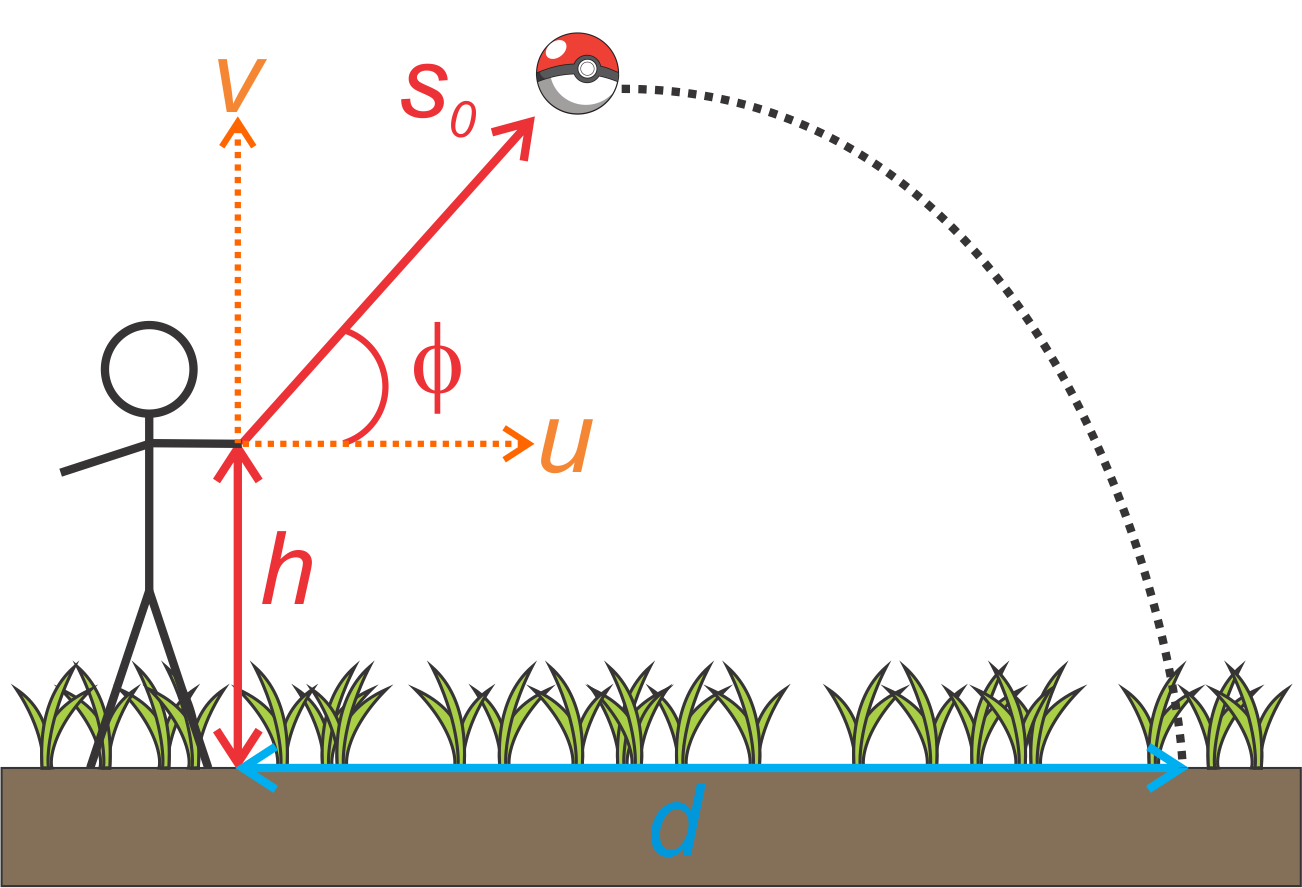
\includegraphics[width=\linewidth]{ch9-ball.png}
\caption{Schematic of the thrown-ball system.}
\label{fig:ch9-ball}
\end{marginfigure}

The system we'll consider is shown schematically in Figure \ref{fig:ch9-ball}. In essence: we want to determine \(d\) -- the horizontal distance (in \(m\)) that the ball travels before it hits the ground. The initial conditions are:
\begin{enumerate}[noitemsep]
\setlength{\itemindent}{.2in}
\item The ball is thrown from an initial height \(h\) (\(m\)).
\item The ball is thrown with an initial speed \(s_{0}\) (\(ms^{-1}\)).
\item The ball is thrown at an initial angle \(\phi\) with respect to the horizontal.
\end{enumerate}
We'll neglect any air desistence or spin imparted to the ball, and for the purpose of calculating its height, we'll ignore its diameter, i.e. we'll consider that the ball is level with the ground when its centre is at height zero. Over and above this, you'll only need to know the gravitational constant (i.e. gravitational acceleration): \(g=9.81 ms^{-1}\) (i.e. the ball is being thrown on an Earth-like planet close to sealevel).

To simply things and the construction of the code and encapsulation of the physics of the model, we'll break it down into 4 steps:

\begin{description}[align=right]

\setlength{\itemindent}{-0.2in}

\item [Part I] Considering only horizontal travel.

\item [Part II] Considering only vertical travel.

\item [Part III] Considering both horizonal and vertical travel and testing for when the ball hits the ground.

\item [Part IV] Add some graphical output.

\end{description}

\vspace{-1mm}
\noindent\rule{4cm}{0.5pt}
\vspace{-2mm}

\begin{marginfigure}[3.0in]
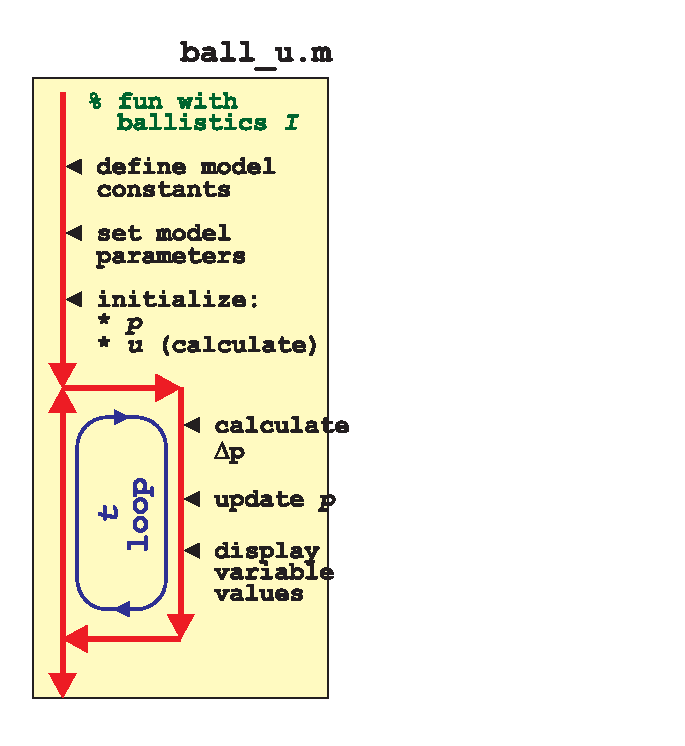
\includegraphics[width=\linewidth]{ch9-schematic-ball_u.eps}
\caption{Schematic of the code for simulating the horizontal movement of a ball.}
\label{fig:ch9-schematic-ball_u}
\end{marginfigure}

\newthought{\textit{\textbf{Part I }}} Start with a new \textsf{m-file} (which can be a simple \textit{script} file). For the structure of the code -- Figure \ref{fig:ch9-schematic-ball_u} is given as an example to guide you. 

First, you are going to need to define a constant (\(g\)) -- the value for gravitational acceleration on Earth. (Here it is termed a 'constant', because its value never changes. The value of \(\pi\) would be another example, although \textbf{MATLAB} provides this as a function return.):
\begin{docspec}
\textcolor[rgb]{0,0.501961,0}{\% model constants}\\
g = 9.81; \textcolor[rgb]{0,0.501961,0}{\% gravitational acceleration (ms-2)}
\end{docspec}

Next, your program needs some parameters (the initial height \(h_{0}\), initial speed (\(s_{0}\)), initial angle (\(\theta\)) of the ball). (These are called parameters because they are invariant during the running of the program, but may be changed if the program is run again.):
\begin{docspec}
\textcolor[rgb]{0,0.501961,0}{\% model parameter values}\\
h0 = 1.0;\\
s0 = ...\\
theta0 = ...;
\end{docspec}
(You might add comments for what the parameters are at the end of the line, and ideally include their units too.)

For now, pick any 'reasonable' values for \(s_{0}\) \sidenote[][-0.0in]{On September 24, 2010, against the San Diego Padres, Chapman was clocked at 105.1 mph (169.1 km/h) -- the fastest pitch ever recorded in Major League Baseball. If you convert 169.1 km/h into units of \(ms^{-1}\), this will give you some reasonable upper limit for your initial  thrown velocity.} and \(\phi\) \sidenote{Obviously, the angle should lie between zero and 90 \degree  (or else the throw is going backwards and/or into the ground). BE CAREFUL as \textbf{MATLAB} assumes that angles are in units of \uline{radians}, so either work in units of radians throughout, or convert from degrees into radians when you calculate the velocity component based on the angle.} (and change the default zero values in the code). (Here, the initial height of the ball is assumed to be \(1m\), but you are free to make a different assumption.)

Then, because you are going to use a time-stepping approach (rather than solving the system analytically), you are going to need to create a loop in time, starting at time zero. Can you guess the time-step you need? No? Then we need to make the time-step a \textit{parameter} that we can change later, to ensure that the system is solved well (i.e. accurately and without numerical instability). You could call this parameter e.g. \texttt{dt} (for \(dt\)) and set it\sidenote{In the parameter definition section of the code.} to an initial (guessed) value such as \(0.1s\). How long should you run the simulation for? This is also a sort of unknown at this point, at least until you have run the simulation a couple of times to get a feel for what the longest time the ball stays in the air might be. So why not pick \(10s\) to start with. Again, create a parameter to hold the value of the maximum model simulation time and assign its value in the parameter definition section of the code, e.g.:
\begin{docspec}
\textcolor[rgb]{0,0.501961,0}{\% model parameter values}\\
...\\
dt \ \ \ = 0.1;\\
max\_t = 10.0
\end{docspec}
(Add comments for what the parameters are and ideally include their units ...)

Assuming a time-step parameter name of \texttt{dt} and a maximum time, \texttt{max\_t}, if your current time is called \texttt{t}, your loop structure will look like:
\begin{docspec}
\textcolor{blue}{for} t = 0:dt:max\_t
\\ \ \ \ \ \textcolor[rgb]{0,0.501961,0}{\%SOME CODE}
\\\textcolor{blue}{end}
\end{docspec}
with time \texttt{t} starting at zero, and progressing to \texttt{max\_t} in steps of \texttt{dt}.

\vspace{1mm}
\noindent\rule{4cm}{0.5pt}
\vspace{2mm}

\noindent What else do you need? You will need to know the horizontal component of the balls velocity.\sidenote[][-2.5in]{In the absence of air resistance, horizontal velocity does not actually change throughout the simulation (i.e. in each iteration of the loop, it will have the same value).}  You can calculate the (initial) horizontal component of velocity (\(u\)) from the given initial conditions of initial speed (\(s_{0})\) and initial angle of trajectory (\(\phi\))\sidenote[][-2.0in]{Just as long as you can remember how to calculate the sides of a right angled triangle given the length of the hypotenuse, which here is the speed. \\REMEMBER that \textbf{MATLAB} uses \textit{radians} for calculating with angles, not \textit{degrees}.} if you can recall your basic trigonometry 101 ... Because this variable (e.g. call it \texttt{u}) depends on parameter values defined at the top of the code, it needs to come after the parameter list, but before the loop starts. 

You also need a variable to represent the horizontal position of the ball (delineated here in the text as \(p\), with units of \(m\)). This will start at zero and be updated within the loop. So also in the variable initial condition section, why not define your horizontal position variable \(p\) and assign it a (initial) value of zero.

The complete section of initializing variables will look like:
\begin{docspec}
\textcolor[rgb]{0,0.501961,0}{\% model initial conditions}\\
u = ...\\
p = 0.0;
\end{docspec}
(here leaving the code for deriving \texttt{u} from \texttt{s0} and \texttt{theta0}, for you to work out ...).

Along with the schematic of the code structure, this should be all you need to create a basic code (but one at this point that does not actually 'do' anything). You should have 1 constant, and then 5 model \textit{parameters} defined representing: the initial height of the ball, the initial speed, and initial angle of throw, plus, maximum time and time step length. Then you should have 2 model variables: (horizontal) position \(p\), which you should have initialized to zero, and  (horizontal) velocity component \(u\), which you should have initialized calculated from \(s_{0}\) and \(\phi\). T\uline{here should be nothing in the loop so far}.

Check that it runs without error even though it is doing nothing useful! Add some debug (e.g. a line in the loop using \texttt{disp}) to check that the loop really does loop from zero to \texttt{max\_t} in steps of \texttt{dt}.\sidenote{Note that depending on whether or not \texttt{max\_t} is divisible by \texttt{dt} with no remainder, your loop might not exactly finish at a value for \texttt{a} of \texttt{dt}.}

Now to add some code to the loop. During each time-step, i.e. each time around the loop, \(dt\) time (\(s\)) passes. (Pause ... and think about this.) In time \(dt\), if the horizontal velocity of the ball is \(u\), you should be able to calculate how far it moves, right?\sidenote{Distance = velocity times time: \\\(dp=u\times dt\)} You need to add this increment in distance travelled to the current value of the position variable \(p\)\sidenote{i.e. with code like 
\begin{docspecmargin}
p = p + dp;
\end{docspecmargin} which you have seen endless times before now and should becoming wearily familiar ...}. Do this (calculating first the change in position, \texttt{dp}, and then updating the position variable, \texttt{p}). (Don't forget to read the margin notes!)

Re-run the code. Check it works at all (if not: debug). Try adding debug code within the loop that displays the current time (\(t\)) plus value of \(p\) at each time-step, e.g.
\begin{docspecmargin}
\textcolor{blue}{for} t = 0:dt:max\_t
\\ \ \ \ \ \textcolor[rgb]{0,0.501961,0}{\%CODE TO UPDATE POSITION}
\\ \ \ \ \ disp(['current time = ', num2str(t), ', ...
\\ \ \ \ \ position = ', num2str(p)]);
\\\textcolor{blue}{end}
\end{docspecmargin}
so that you can track what is going on. (You can make a fancier output if you wish and add in the relevant units to the output.)

Strictly, when updating the position of the ball in the first iteration of the loop, time is \(dt\) at this point, not zero, which is what the loop thinks (you already have a position of zero at time zero -- the initial conditions). So rather than starting the loop at zero,  modify the loop to start instead at a value of \(dt\).

You should have a working model at this point, albeit only for the horizontal position of the ball.

\vspace{1mm}
\noindent\rule{4cm}{0.5pt}
\vspace{-2mm}

\newthought{\textit{\textbf{Part II }}} Now for tracking the vertical position (and velocity) of the ball. Copy and rename your previous \textsf{m-file} -- use this as a starting point for the new model. You are going to modify your program so that \(p\) is now the vertical, not horizontal, position of the ball.

\begin{marginfigure}[1.25in]
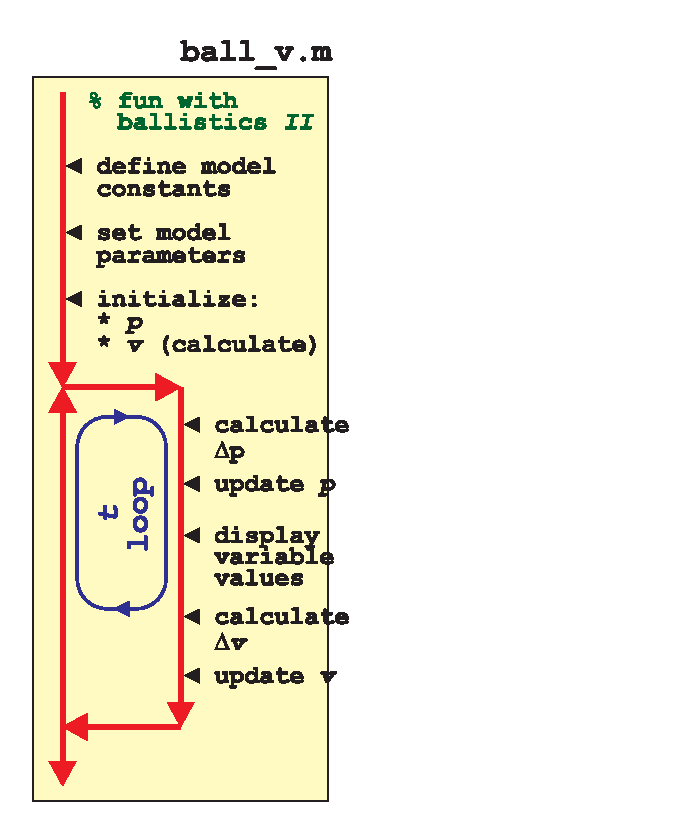
\includegraphics[width=\linewidth]{ch9-schematic-ball_v.eps}
\caption{Schematic of the code for simulating the vertical movement of a ball.}
\label{fig:ch9-schematic-ball_v}
\end{marginfigure}

Think about what is different about the physics of the system (Figure \ref{fig:ch9-ball}) from before -- this is going to directly inform how you adjust and add to the code. To start with, you should have noticed that the initial position (\(p_{(0)}\)) of the ball does not start at zero, but rather at height \(h_{0}\) (see Figure \ref{fig:ch9-ball}). This is one change to make in the code (i.e. having defined \(h_{0}\) as a parameter, you subsequently use \(h_{0}\) to set the initial value of \(p\)). Also -- the initial (vertical) velocity component, which we will call \(v\) (rather than \(u\) which we used for the horizontal velocity), is different from before. So go back to your triangle trigonometry,  and calculate of the initial vertical velocity component (\(v_{0}\)). Overall, the code structure looks like Figure \ref{fig:ch9-schematic-ball_v}.

You could, and indeed should, test the code so far. It should in fact do something very similar to before, with position \(p\) increasing, linearly, as a function of time (i.e. as the loop progresses in the number of iterations carried out). The only differences you should see are that \(p\) starts from value \(h_{0}\) and the rate at which \(p\) changes will be greater or less than before, depending on the value of \(\theta\) you assumed.\sidenote{What value of \(\theta\) would result in an \uline{identical} change in \(d\) with time (comparing the previous horizontal-only model with the new vertical (only) one)?}

So far so good. Except balls generally do not continue travelling vertically upwards for ever. You are missing gravity in this (vertical-only) model. Your variable for \(v\) (vertical velocity) now needs to change as a function of time and you'll need to update its value within the loop\sidenote{\uline{Before} or \uline{after} the updating the position? Actually, a slightly tricky question.}.

How are you going to update \(v\)? Well, the change in velocity with time is called acceleration and in this example the only force exerting any acceleration on the ball is gravity. Mathematically we can approximate the change in velocity, \(\Delta v\) as:
\begin{docspec}
\(\Delta v=-\Delta t\cdot g\)
\end{docspec}
where \(g\) is the acceleration due to gravity. Note the appearance of a minus sign in the equation if we are considering a coordinate system with distance upwards.

So in the loop, calculate the change in velocity during the time-step, and then update the value of \(v\)\sidenote[][-0.0in]{Hint:
\begin{docspecmargin}
\(v_{(t+1)}=v_{(t)}+\Delta v\)
\end{docspecmargin} where \(v_{(t+1)}\) is the new (at the next time-step) velocity and  \(v_{(t)}\) the current velocity}.\sidenote{Note that in this example and as per Figure \ref{fig:ch9-schematic-ball_v}, we update the vertical position in the loop \uline{first} (at the start of the loop), and then update the velocity afterwards.} You should end up with 5 lines in the loop (excluding comments):
\begin{enumerate}[noitemsep]
\setlength{\itemindent}{.2in}
\item Calculate the change in position (\texttt{dp}), based on the current (vertical) velocity, \texttt{v} and the increment in time (\texttt{dt}).
\item Update the position \texttt{p} based on the current value of the position, plus the change in value (\texttt{dp}).
\item A line of debug to display the current (loop) time and the current position.
\item Calculate the change in velocity (\texttt{dv}), based on gravitational acceleration and the increment in time (\texttt{dt}).
\item Update velocity \texttt{v} based on the current value of velocity, plus the change in value (\texttt{dv}).
\end{enumerate}

Re-run the model ... what happens? Does this seem 'reasonable' (i.e. how the position changes as a function of time)?\sidenote{You might think about your own direct experience with throwing balls, as a reality check. i.e. have you ever thrown one that took a minute to come down, or one that hit the ground within 0.1s? If these sorts of things happen in the model, you may have a bug in there somewhere.} At this point you might consider whether you really do need to run the model for as long as \(10s\). Play about with the assumed initial angle and also the velocity and get a feel for what is the longest the ball lasts in the air (i.e. until its position becomes negative). 

\vspace{1mm}
\noindent\rule{4cm}{0.5pt}
\vspace{-2mm}

\newthought{\textit{\textbf{Part III }}} By now, you should now have 2 working models (sperate \textbf{m-files}) -- one for the horizontal position of the ball, and one for the vertical position (and vertical velocity) of the ball. You now want to combine the 2 sperate parts of the model.\sidenote{I suggest basing the combined model on the vertical model (as it is the more complicated of the 2) and hence copying-and-renaming the 2nd script (i.e. so you end up with 3 different \textbf{m-files} in the end).}

How to merge? Mostly, the code content of the 2 individual models was  identical, but there is more in the vertical position model, so that would be the better one to copy and rename. Then what you need to copy across from the horizontal model and add in is:
\begin{itemize}[noitemsep]
\setlength{\itemindent}{.2in}
\item The calculation of the initial value of \(u\).
\item The initialization of the horizontal position.
\item The calculation of the change in horizontal position each time-step.
\item The updating of the new horizontal position.
\end{itemize}

By now, you should have noted a slight problem -- in both previous (sperate) models, the variable \(p\) was used to represent both the horizontal AND vertical position of the ball. \docenvdef{D'uh!}\marginnote{
\docenvdef{duh}
\\\textit{exclamation informal}
\\used to comment on an action perceived as foolish or stupid, or a statement perceived as obvious. As in:
\\"I used the same variable name twice and which is why the model did not work -- duh!"
}

My solution would be ... a vector, to store the current position -- just of one row and two columns, i.e. exactly as you might write a position in \((x,y)\) notation. The horizontal position (\(x\)) is hence assigned the first element (\texttt{p(1)}) and the vertical position, the 2nd (\texttt{p(2)}). If you do this (i.e. resolve the variable clash this way), you'll need to edit how you set the initial conditions in the code, e.g.
\begin{docspec}
p(1) = 0;
\\p(2) = h0;
\end{docspec}
as well as how the position is updated in the loop. You can leave the name of the increment in position (\(\Delta p\)) the same if you wish (as this is a temporary variable whose value is replaced each time around the loop in any case), e.g.
\begin{docspec}
\ \ \ dp = dt*u;\\
\ \ \ p(1) = p(1) + dp;\\
\ \ \ dp = dt*v;\\
\ \ \ p(2) = p(2) + dp;
\end{docspec}
where the 1st 2 lines calculate the change in horizontal position and then update the \(x\) (\texttt{p(1)}) component of position, and the 2nd 2 do the same only for the \(y\) (\texttt{p(2)}) component of position. 

Hopefully this works and runs ... Maybe add some output within the loop to track its progress, such as:
\begin{docspecmargin}
\textcolor{blue}{for} t = 0:dt:max\_t
\\ \ \ \ \ \textcolor[rgb]{0,0.501961,0}{\%CODE TO UPDATE POSITION}
\\ \ \ \ \ disp([\textcolor[rgb]{1,0,1}{'('}, num2str(p(1)), \textcolor[rgb]{1,0,1}{','}, ...
\\ \ \ \ \ num2str(p(2)), \textcolor[rgb]{1,0,1}{') @ t = '}, num2str(t)]);
\\\textcolor{blue}{end}
\end{docspecmargin}

You should end up with output, depending on how you constructed the string to be displayed by \texttt{disp} (and what initial conditions you chose ...), like:
\begin{docspecmargin}
>> ball\_uv
\\(0.5,1.866) @ time 0.1
\\(1,2.634) @ time 0.2
\\(1.5,3.3038) @ time 0.3
\\(2,3.8755) @ time 0.4
\\(2.5,4.3491) @ time 0.5
\\(3,4.7247) @ time 0.6
\\(3.5,5.0021) @ time 0.7
\\(4,5.1814) @ time 0.8
\\(4.5,5.2626) @ time 0.9
\\(5,5.2458) @ time 1
\\(5.5,5.1308) @ time 1.1
\\(6,4.9177) @ time 1.2
\\(6.5,4.6065) @ time 1.3
\\(7,4.1973) @ time 1.4
\\(7.5,3.6899) @ time 1.5
\\(8,3.0844) @ time 1.6
\\(8.5,2.3808) @ time 1.7
\\(9,1.5792) @ time 1.8
\\(9.5,0.67938) @ time 1.9
\\(10,-0.31849) @ time 2
\\(10.5,-1.4145) @ time 2.1
\\ \ldots 
\\ \ldots 
\end{docspecmargin}
which is far far far from exciting ... but does at least confirm a constant change in horizontal position with time, and a vertical position that initially increases above the initial condition (\(h_{0}=1.0\)) but subsequently drops back and eventually falls below zero. And the time at which the vertical position reaches zero, is the value of \(d\) in  Figure \ref{fig:ch9-ball}.

The very least we could do at this point is to detect when the ball has reached the ground and terminate the loop. I'll leave this code for you to devise, but you'll need:
\begin{enumerate}[noitemsep]
\setlength{\itemindent}{.2in}
\item A conditional statement (\texttt{if ...}) to test whether the vertical position (\texttt{p(2)}) has dropped below zero. This would go in the loop just after the position of the ball has been updated, and  ...
\item ... within the conditional, the \textbf{MATLAB} command to exit a loop, which you have seen before (look it up if you have forgotten!).
\end{enumerate}

Now you might note that when the ball reaches the ground (technically: its height falls below zero) and the loop exists, you may already be way below zero. In fact, if you are even the least little bit observant, you might note that the change in height per time-step at the end of the simulation is quite large (order meters) and hence it is unlikely you'll ever capture the moment that the ball is very close to the ground. Unless you shorten the time-step, that is. So play about with a shorter time-step (you only need change the value you assigned to the parameter representing \(\Delta t\) in the code). How short does it have to be in order to catch the moment the ball reaches the ground (passes zero) to within e.g. \(0.1 m\)?\sidenote{i.e. to have the loop terminate when the height is no more than \(-0.1 m\).} What about \(0.01 m\)? 

In terms of how long the model takes to run and how many time-steps it uses -- is it even 'worth' finding when the ball hits the ground to an accuracy of \(0.01 m\)? What is the difference in the value of \(h\) you determine between different assumptions about the time-step? As you increase the length of the time-step, when does the value of \(d\) start to appreciably change (compared to assuming a very short time-step)? This is a measure of 'error' associated with the assumed time-step duration. Think about whether the error in \(d\) is 'meaningful' compared to \(d\) itself.

\newthought{\textbf{\textcolor{red}{OPTIONAL}} -- Finally --} as an alternative to creating a \texttt{for} loop in which we pre-defined a maximum number of time-steps (or maximum time) and then  had to exit the loop once the ball reaches zero height about the ground, try re-writing the loop as a \texttt{while} loop, with the condition (for the loop to continue looping) that the ball has a height above the ground that is greater than zero. (This makes for a much neater solution to the problem.)

\vspace{1mm}
\noindent\rule{4cm}{0.5pt}
\vspace{2mm}

\newpage

\newthought{\textit{\textbf{Part IV }}} Some graphics fun.

It would be kinda fun (really) to show the ball 'flying through the air'. There are a variety of ways of doing this. We'll start with the simplest first and use \texttt{scatter}.

As a departure from previous plotting, we don't want to plot at the very end (after the loop)\sidenote{Although if you stored the position of the ball at each time-step, you could re-play the trajectory afterwards.} but rather, plot each position as it is calculated, within the loop.

In the code -- open a new graphics figure window, before the loop starts, and set \texttt{hold on}, by adding the lines
\begin{docspec}
figure;
\\hold on;
\end{docspec}

Within the loop, you want to plot each \((x,y)\) position as it is calculated (\uline{after} the position has been updated, that is) by:
\begin{docspec}
\ \ \ \ scatter(p(1),p(2));
\end{docspec}
(feel free to add additional parameters to \texttt{scatter} to make the points smaller or larger, or filled, or whatever). Comment out any debug (\texttt{disp)} lines.

Well, not so exciting. The plots sort of appears all at once and there is no sense of animation or of the ball moving. \textbf{MATLAB} is just way too fast for its own good\sidenote{This is a Trump-ism. In truth, \textbf{MATLAB} is about the slowest piece of *\$\&\% about.}.

You can make the loop proceed slower, by adding a time delay -- i.e. each time around the loop, \textbf{MATLAB} will take whatever time it needs to carry out the calculation and plot the current position PLUS whatever additional time you tell it to chill out for. The command is \docenvdef{pause} and you might initially try e.g.
\begin{docspec}
\ \ \ \ pause(0.05);
\end{docspec}
which should insert a \(50 ms\) delay into the loop. Place this line just after \texttt{scatter}. Run it.

\marginnote[-1.0in]{\begin{mdframed}[backgroundcolor=gray!10, roundcorner=10pt,leftmargin=1, rightmargin=1, innerleftmargin=5, innerrightmargin=5, innertopmargin=5,innerbottommargin=5, outerlinewidth=1, linecolor=light-gray]
\docenvdef{pause}
\\\textbf{MATLAB} says: "\textit{\texttt{pause(mjs)} pauses the MATLAB job scheduler's queue so that jobs waiting in the queued state will not run.}"
\\Garbage.
\\\texttt{pause(n)} will pause the execution of the code by \texttt{n} seconds.
\end{mdframed}}

Now it has all got really trippy. If you tell it no different, \texttt{MATLAB} insists on auto-scaling the (\(x\) and \(y\) limits of the) plot. As the position of the ball increases (initially) in \textit{y}-axis direction, and (constantly) along the \textit{x-axis} direction, \textbf{MATLAB} periodically re-scales the axes. Annoying. So before the loop starts and after you create the figure window, why not prescribe axes limits(?) Having played with the model you should have a reasonable idea for what the maximum vertical and horizontal distances are associated with 'reasonable' choices for the initial conditions (\(s_{0}\) and \(\theta\)).\sidenote[][-1.0in]{Don't forget the command for specifying a scale for the axis limits is \texttt{axis}.} You should end up with something like Figure \ref{fig:ch9-ball_uv} once the program has completed.

\begin{marginfigure}[-0.5in]
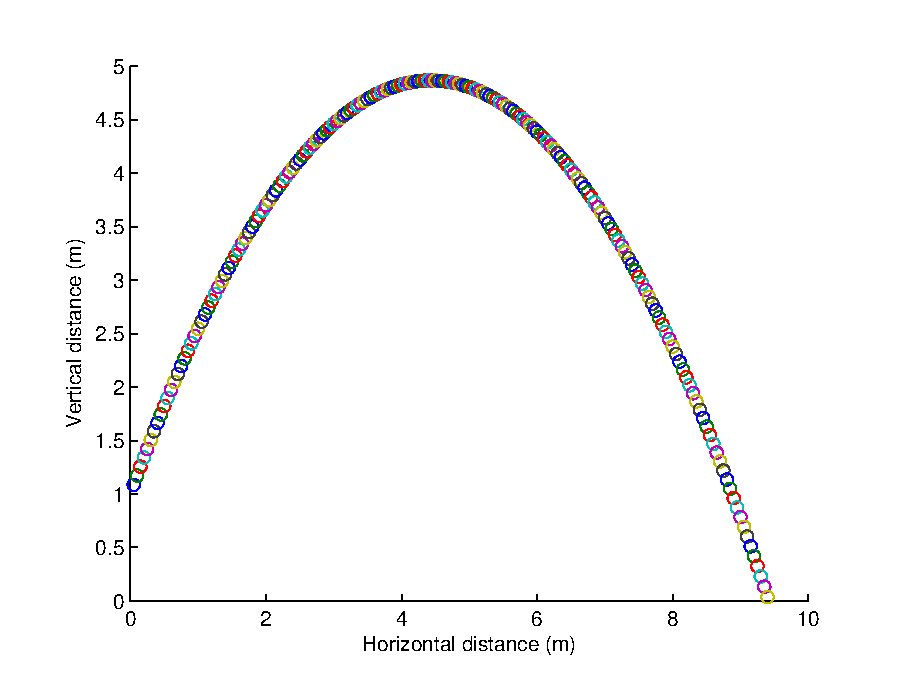
\includegraphics[width=\linewidth]{ch9-ball_uv.eps}
\caption{Trajectory of a ball!!}
\label{fig:ch9-ball_uv}
\end{marginfigure}

\newpage 

\newthought{\textbf{\textcolor{red}{OPTIONAL}} -- Also --} try turning your script into a function so that you do not need to edit the values of \(s_{0}\) and \(\theta\) in the code, but pass them into the program as parameters instead (the function needs not return anything however).

\vspace{1mm}
\noindent\rule{4cm}{0.5pt}
\vspace{2mm}

\noindent Having developed some visualization for the trajectory of the ball, this is a good point to experiment with the length of the time-step and determine at what point (time-step duration) the numerical approximation starts to break down -- i.e. as compared to a simulation with a very short time-step (or an analytical solution), when (what longer time-step duration) does the trajectory start to visually differ (and the distance travelled before the ball hits the ground, change)? e.g. Figure \ref{fig:ch9-ball_uv2} illustrates a \(0.1s\) time-step and Figure \ref{fig:ch9-ball_uv3} a \(0.2s\) time-step (contrast with Figure \ref{fig:ch9-ball_uv}).

\begin{marginfigure}[-0.0in]
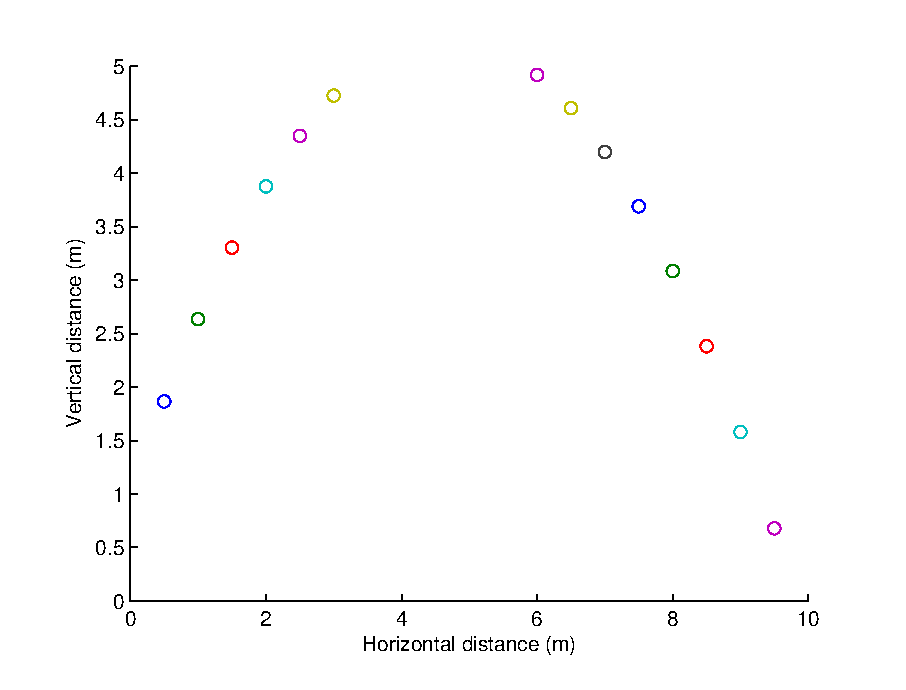
\includegraphics[width=\linewidth]{ch9-ball_uv2.eps}
\caption{Trajectory of a ball (with a poor time-step choice).}
\label{fig:ch9-ball_uv2}
\end{marginfigure}

\begin{marginfigure}[-0.0in]
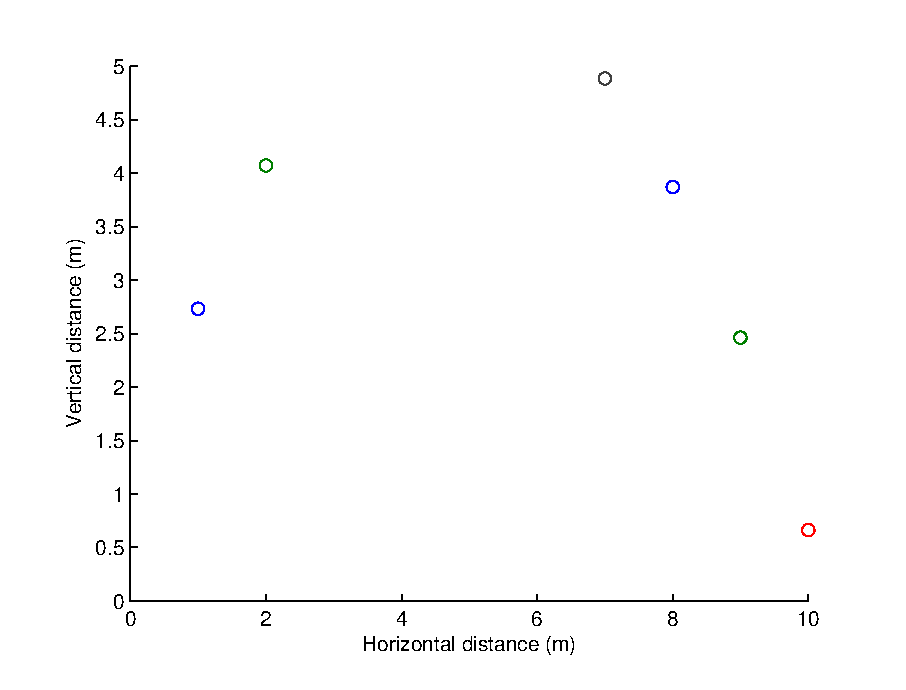
\includegraphics[width=\linewidth]{ch9-ball_uv3.eps}
\caption{Trajectory of a ball (even poorer time-step choice).}
\label{fig:ch9-ball_uv3}
\end{marginfigure}

\vspace{1mm}
\noindent\rule{4cm}{0.5pt}
\vspace{2mm}

\noindent If you are keen ... you can make more of an 'animation' out of the ball trajectory plotting. One trick would be to re-plot the position of the ball a second time, but now in white (hence covering up the previous drawing). Better is to ask \textbf{MATLAB} to delete the last ball object.

When you call \texttt{scatter} as a function, a \textit{handle} is returned that is the ID of the points plotted. You can use this ID to delete the point again! e.g. close all the currently open windows and try the following:
\begin{docspec}
>> h=scatter(1,2);
\end{docspec}
and you get a circle plotted at location \((1,2)\).
\begin{docspec}
>> delete(h);
\end{docspec}
... and ... it is gone (but leaving (re-scaled) axes in place).

If, in your loop, after updating the position of the ball, you have:
\begin{docspecmargin}
\ \ \ h=scatter(p(1),p(2),50,\textcolor[rgb]{1,0,1}{'filled'}, ...\\
\ \ \ \ \ \ \textcolor[rgb]{1,0,1}{'MarkerFaceColor'},[1 0 0],\textcolor[rgb]{1,0,1}{'MarkerEdgeColor'},[0 0 0]);\\
\ \ \ pause(0.025);\\
\ \ \ delete(h);
\end{docspecmargin}
you should see a red ball (with a black outline) smoothly sailing across the screen.\sidenote[][-1.0in]{You could make the animation a little smoother by decreasing the time-step and also playing about with the delay (\texttt{pause}).}
\sidenote[][-0.25in]{
A slight complication here as that as it stands, the code will not work because in the first time around the loop, when you get to \texttt{delete(h)}, \textbf{MATLAB} is unhappy because the \textit{handle} \texttt{h} has not yet been defined anywhere.
The easiest way to fix this is outside the loop, to plot the initial position of the ball (and obtain its \textit{handle}). e.g.:
\begin{docspecmargin}
figure;\\
axis([0 10 0 5]);\\
hold on;\\
h=scatter(p(1),p(2),50,'filled');
\end{docspecmargin}
Now when the loop starts, there is a 'ball' to delete!
}

\vspace{1mm}
\noindent\rule{4cm}{0.5pt}
\vspace{-2mm}

\newthought{\textbf{\textcolor{red}{OPTIONAL}} -- A further refinement} would be to add a term to account for air resistance -- as the ball travels through the air, friction will act to decelerate the ball. 

You could represent the effect of friction in a similar way to how you accounted for gravity, except (a) friction will affect both velocity components, and (ii) friction will act to decelerate the ball, regardless of its direction of travel (up or downwards). Friction also differs from gravitational acceleration in that the deceleration will not be constant, but instead a function of velocity. Furthermore, can assume that friction will scale with the square of the velocity (rather than linearly).

In your basic code:
\begin{docspec}
\ \ \ dp = dt*u;\\
\ \ \ p(1) = p(1) + dp;\\
\ \ \ dp = dt*v;\\
\ \ \ p(2) = p(2) + dp;\\
\ \ \ dv = -dt*g;\\
\ \ \ v = v + dv;
\end{docspec}
you would add (to the end of the loop):
\begin{docspec}
\ \ \ du = -dt*f*u\(^{\wedge}\)2;\\
\ \ \ u = u + du;\\
\ \ \ dv = -dt*f*v\(^{\wedge}\)2;\\
\ \ \ v = v + dv;
\end{docspec}

Here, \texttt{f} is a parameter that scales the impact of air resistance on velocity. It is not clear, at least in this simplistic formulation, what its value should be. So this (the value of \texttt{f}) is something to explore and test the effect of.

%------------------------------------------------

\newpage

%------------------------------------------------

\section{Dynamics in the zero-D Energy-balance climate model}

In this next Example making use of time-stepping, we will make the zero-D energy-balance climate model (very) slightly more interesting, or at least, (very) slightly more realistic.

The time-dependent behavior of the initial version of the energy balance model is trivial. In fact: there isn't any. The system is always in equilibrium as constructed. Why? No thermal inertia -- i.e. nothing in the physical system as defined in the equations  has  any heat capacity and the outgoing (long-wave / infrared) energy flux is always assumed to be in exact equilibrium with the incoming (shortwave) flux. So we need to add an ocean, or rather: a box (a \textit{variable} in the \textbf{MATLAB} code) to store the heat content, or temperature, of the ocean, and update this (temperature) in the event of there being any imbalance between gain and loss of energy at the surface of the Earth.

\marginnote[-2.75in]{\begin{mdframed}[backgroundcolor=gray!20, roundcorner=10pt,leftmargin=1, rightmargin=1, innerleftmargin=5, innerrightmargin=5, innertopmargin=5,innerbottommargin=5, outerlinewidth=1, linecolor=light-gray]
\textbf{Specific Heat Capacity}
\\According to wikipedia: "\textit{An object's }[or here: ocean]\textit{ heat capacity (symbol C) is defined as the ratio of the amount of heat energy transferred to an object and the resulting increase in temperature of the object:}" 
\begin{docspecnormal}
\(C=\frac{Q}{\Delta T}\)
\end{docspecnormal}
where \(Q\) is the (change in) energy (so could equally be written \(\Delta Q\) if you prefer) and \(\Delta T\) the associated change in temperature. Units are:
\begin{itemize}[noitemsep]
\setlength{\itemindent}{.2in}
\item \(C\) --- \(J K^{-1}\)
\item \(\Delta T\) --- \(K\)
\item \(Q\) --- \(J\)
\end{itemize}
Typical units for specific heat capacity are:
\\\(Jg^{-1}K^{-1}\)
\\(or \(Jkg^{-1}K^{-1}\))
\end{mdframed}}

The science behind the new model is based directly on the basic energy balance equations you had before, except this time, you are not going to assume that the 2 equations are equal (and hence solve for \(T\)). Instead, you are going to calculate the net energy gain (or loss) over a given interval of time and use the \uline{specific heat capacity} of a substance (assuming water here)\sidenote[][-0.5in]{Once again -- be very careful with the units. Or all will be lost ...} to link this energy change, to a temperature change (see Box). This will be the basis of the 'dynamics' of the climate model and will dictate how quickly the mean surface temperature responds to any imbalance in loss vs. gain of energy. 

You will  assume the following:
\begin{itemize}[noitemsep]
\setlength{\itemindent}{.2in}
\item The average mixed layer depth of the ocean is 70 m.
\item The average fraction of the Earths surface that is ocean is 0.7.
\end{itemize}
(both from \textit{Henderson-Sellers} [2014]) -- Figure \ref{fig:ch8-ebm}. You'll also need to know:
\begin{itemize}[noitemsep]
\setlength{\itemindent}{.2in}
\item The specific heat capacity of water.
\end{itemize}
(see Box) but you can find this out for yourself ... Note that you do not need to know e.g. the radius of the Earth as we are constructing the model on a global average per \(m^{-2}\) basis as before (i.e. we are considering a representative \(1 m^{2}\) of surface, of which \(70\%\) is water (or \(0.7 m^{2}\)) with a depth of \(70m\).

\begin{marginfigure}[-5.0in]
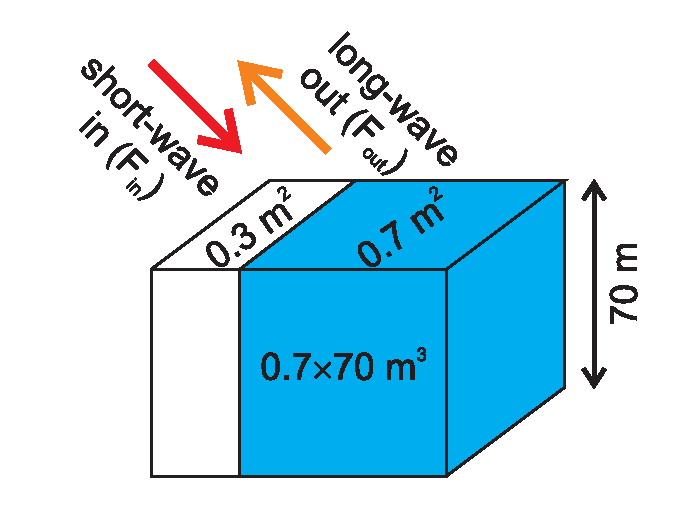
\includegraphics[width=\linewidth]{ch8-ebm.eps}
\caption{Schematic of the dynamic EBM.}
\label{fig:ch8-ebm}
\end{marginfigure}

\begin{marginfigure}[-1.5in]
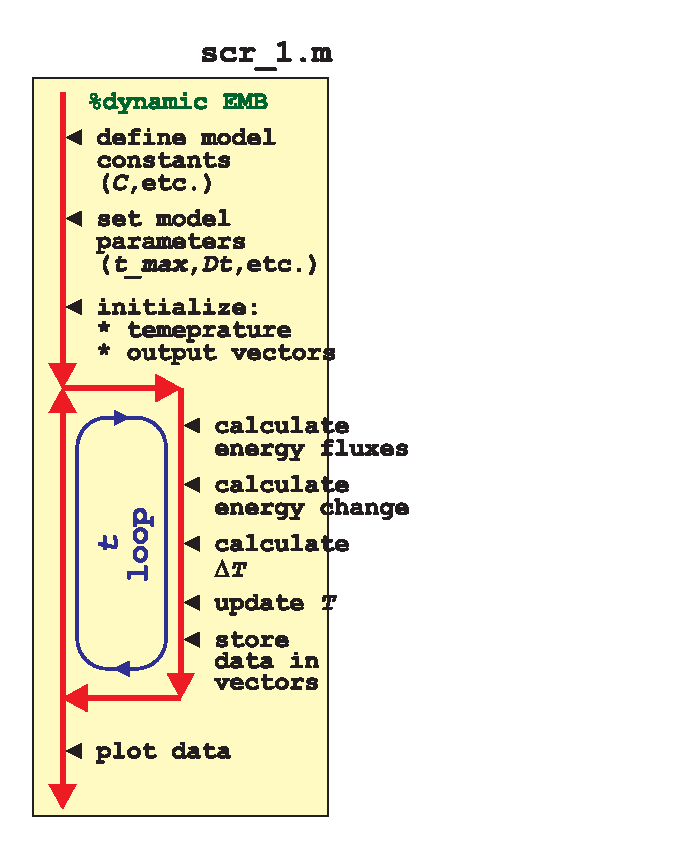
\includegraphics[width=\linewidth]{ch9-schematic-scr1.eps}
\caption{Schematic of the script for the basic dynamic EBM}
\label{fig:ch9-schematic-scr1}
\end{marginfigure}

The form of the program is shown schematically in Figure \ref{fig:ch9-schematic-scr1}. You'll need to create yourself a new script (\texttt{scr\_1}) to make this. Much of this and the main sections of code should look familiar. Break the code down into logical sections. Start by defining any constants you need, as well as parameter values. For the time loop, we are going to start off with a fixed total duration and a fixed time step (a little later, we'll relax these constraints). And to make things really simple to start -- assume a \(100\) year duration (starting at \(T=1.0\)) and a loop time increment , \(\Delta T=1.0\) (year). So you are not even going to need to initialize and update a loop counter in the code! 

In the loop itself, you firstly need to calculate the energy imbalance (assuming there is one) between incoming solar radiation absorbed  and out-going infrared radiation loss. For this -- taken the equations given to you earlier for absorbed solar radiation and infrared loss, and simply calculate the difference (rather than re-write in terms of \(T\) as you did for the equilibrium EBM) -- \(\Delta F\).

From the energy flux imbalance (\(\Delta F\)), which is in units of \(Wm^{-2}\), i.e. \(Js^{-1}m^{-2}\), you'll need to calculate how many \(J\) of energy (per \(m^{2}\)) are lost or gained over the course of your time-step. Your time-step is in units of years ... so you'll need to calculate how many \(s\) in a (average) year, and multiply the energy change \(s^{-1}\) by this number (to give the energy change per time-step). The energy change can then be used to update the temperature of the mixed layer ocean ... as long as you have already calculated the heat capacity of the ocean that is ...\sidenote[][-3.0in]{
Assuming specific heat capacity is in units of \(Jg^{-1}K^{-1}\), you need to find the mass of the ocean box in \(g\), noting that the density of (pure water at 0C) is \(1\:gcm^{-3}\).
\\Start by determining the volume of the ocean box in \(cm3\), convert to \(g\), and then multiply the specific heat capacity \(C\) by this, to give the heat capacity of the ocean box.
\\This is the number of \(J\) of energy needed to raise the temperature by \(1K\).
}.

A possible sequence of calculations (assuming you have calculated the heat capacity of the ocean box once, before the loop starts) follows\sidenote[][-1.5in]{It is much easier and less prone to bug, if you split things into five steps.}:
\begin{enumerate}[noitemsep]
\setlength{\itemindent}{.2in}
\item Calculate incoming energy flux, \(F_{in}\).
\item Calculate outgoing energy flux, \(F_{out}\).
\item Calculate the net energy change (per \(m^{2}\) per \(s\)) at the Earths surface, \(\Delta F\).
\item Calculate the total energy imbalance (per \(m^{2}\)) over a year, in \(J\).
\item Using the heat capacity of the 'ocean' , calculate its temperature change.
\end{enumerate}
After the loop, plot something helpful at the end. 
If successful, you should see something similar to (actually, identical to) Figure \ref{fig:ch4-ebm-model1} (assuming a \(1\:yr\) time-step).

\begin{marginfigure}[-4.0in]
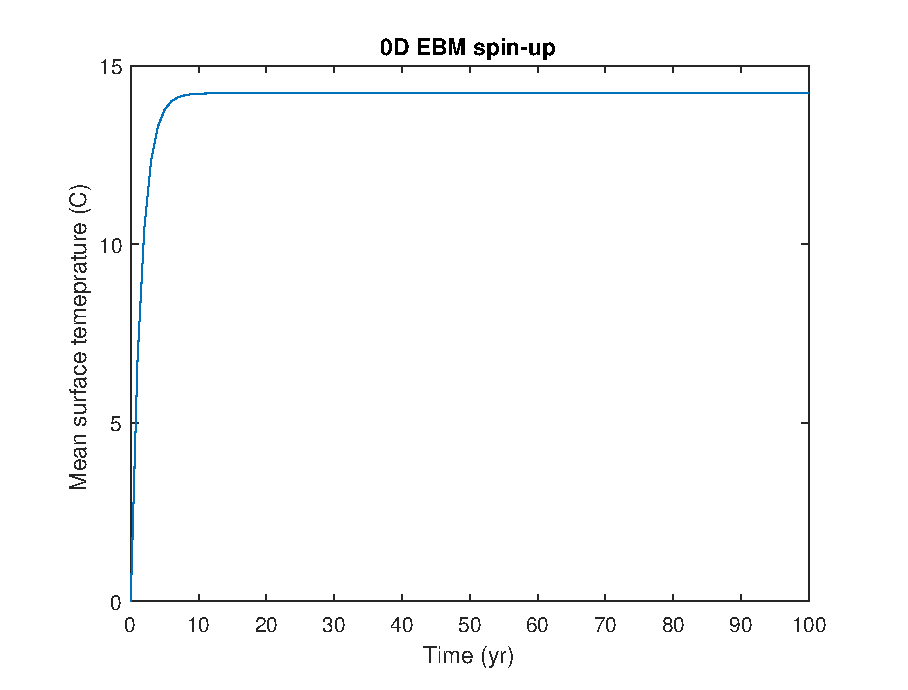
\includegraphics[width=\linewidth]{ch4-ebm-model1.eps}
\caption{100 yr spin-up of the basic EBM.}
\label{fig:ch4-ebm-model1}
\end{marginfigure}

\vspace{1mm}
\noindent\rule{4cm}{0.5pt}
\vspace{2mm}

\begin{marginfigure}[-1.0in]
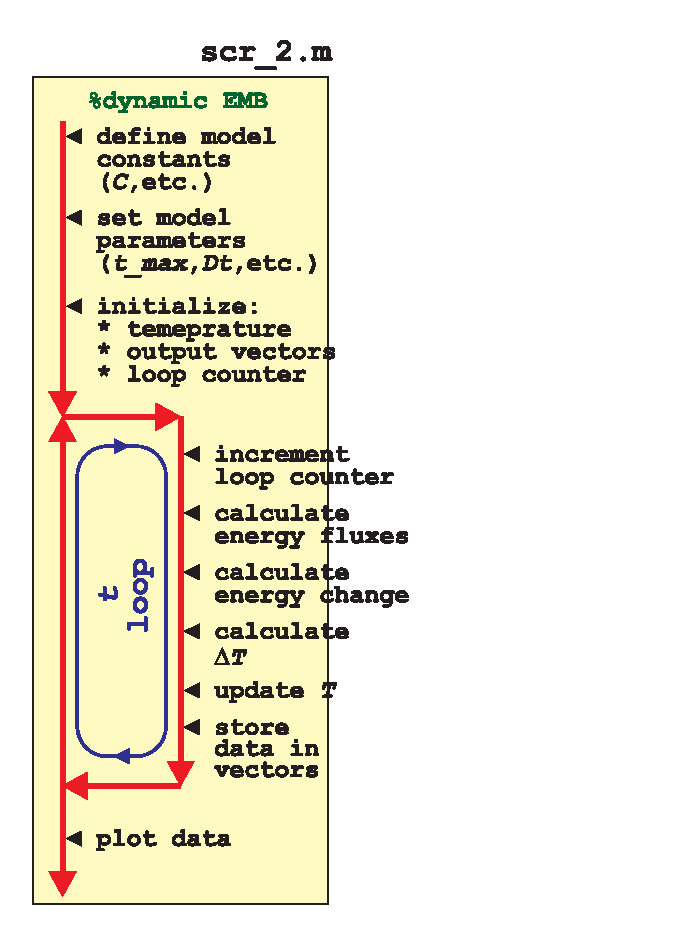
\includegraphics[width=\linewidth]{ch9-schematic-scr2.eps}
\caption{Schematic of the script for the basic dynamic EBM -- now with added loop count(!)}
\label{fig:ch9-schematic-scr2}
\end{marginfigure}

\noindent Next, you are going to play a little with the time-step in the model. So, rather than a simple loop from \(1\) to \(100\) (years) with an increment of \(1\), you are going to generalize  the increment as \(\Delta t\). If \texttt{dt} is your parameter representing the increment in time (presumably, conveniently defined hear the start of the code)\sidenote[][-0.0in]{Don't forget to convert \texttt{dt} into units of \(s\) when you use it in the energy calculation.}, and \texttt{max\_t} the maximum time (here: 100 years) (also conveniently defined near the start of the code?), then:
\begin{docspec}
\textcolor[rgb]{0,0.501961,0}{\% start of time-stepping loop}
\\\textcolor{blue}{for} t = dt:dt:max\_t,
\\ \ \ \ \ \textcolor[rgb]{0,0.501961,0}{\% SOME CODE GOES HERE}
\\\textcolor{blue}{end}
\end{docspec}
Now you will need to crete yourself a loop counter in order to store the results (for subsequent plotting),  because \texttt{dt} will not necessarily be an integer and hence you will not be able to use \texttt{t} to index your data storage vector (/array). The modification needed is only minor however -- see Figure \ref{fig:ch9-schematic-scr2}.

The only slight complication is in knowing the size of the output vectors, assuming that you have created them (using \texttt{zeros}) up-front in the code (and as per the Figure \ref{fig:ch9-schematic-scr1} schematic), rather than growing the vectors as the loop progresses (see earlier). Initially, you would have been able to simply write e.g.
\begin{docspec}
\ \ \ \ data\_time \ = zeros(100,1);
\\ \ \ \ \ data\_T = zeros(100,1);
\end{docspec}
 One strategy is simply to pick a  number larger than you think the number of times the loop will execute. The downside being that you might create a vast array with only a small portion of it ever being used. Better in this example would be to append to the vectors as the loop progresses and not attempt to define them beforehand (i.e. Figure \ref{fig:ch9-schematic-scr1} rather than Figure \ref{fig:ch9-schematic-scr2}).  

By playing around with different parameter values for \(\Delta t\), you should discover that some care has to be taken with the choice of time-step duration, e.g. Figure \ref{fig:ch4-ebm-model2} has a time-step of 3.5 years, which clearly is on the verge of going doolally. \sidenote[][-4.0in]{For practice (fun!?), you could turn the script into a function. Make two parameters as inputs: (1) the total simulation duration, and (2) the time-step, both in units of yr.}

\marginnote[-3.0in]{\begin{mdframed}[backgroundcolor=gray!30, roundcorner=10pt,leftmargin=1, rightmargin=1, innerleftmargin=5, innerrightmargin=5, innertopmargin=5,innerbottommargin=5, outerlinewidth=1, linecolor=light-gray]
\textbf{Doolally}
\\Mad, insane, eccentric.
\end{mdframed}}

\begin{marginfigure}[-2.0in]
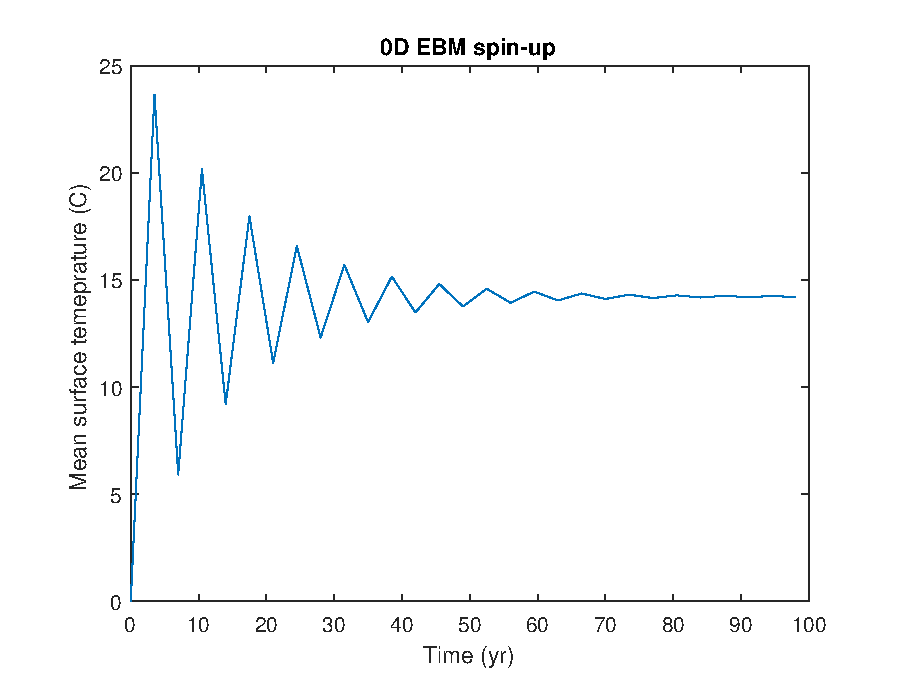
\includegraphics[width=\linewidth]{ch4-ebm-model2.eps}
\caption{100 yr spin-up of the basic EBM, but with a poor choice of time-step ...}
\label{fig:ch4-ebm-model2}
\end{marginfigure}

So far, so far from exciting -- you have been simply time-stepping the model to equilibrium, for which there was an analytical solution anyway (with ocean heat capacity irrelevant to this). However, it should be apparent that it takes some years (how many) for the system to reach equilibrium. This would have important implications for a (real world) system in which the one of the terms in the radiative balance equation changes relatively rapidly (or on a time-scale comparable to the adjustment time of the system). The concentration of CO\(_{2}\), and radiative forcing due to the 'greenhouse effect', is just such an example.

\vspace{1mm}
\noindent\rule{4cm}{0.5pt}
\vspace{-2mm}

\newthought{A follow-on Example to this}, takes the time-stepping (dynamic)  zero-D EBM and calculates the warming impact of a prescribed  CO\(_{2}\) concentration (technically: mixing ratio) in the atmosphere.

\marginnote[-2.0in]{\begin{mdframed}[backgroundcolor=light-blue, roundcorner=10pt,leftmargin=1, rightmargin=1, innerleftmargin=5, innerrightmargin=5, innertopmargin=5,innerbottommargin=5, outerlinewidth=1, linecolor=light-gray]
\textbf{The Greenhouse Effect}
\\The effect of changing CO\(_{2}\) concentrations on the global energy budget is typically written in terms of a virtual (long-wave) radiation flux applied at the top of the atmosphere. The flux anomaly, \(\Delta F\), as a function of CO\(_{2}\) concentration (technically: mixing ratio) (\(CO_{2}\)) relative to a reference (pre-industrial) concentration (typically: \(CO_{2(0)}=278 ppm\)) can be approximated:
\begin{docspecnormal}
\(\Delta F=5.35\cdot ln(\frac{CO_{2}}{CO_{2(0)}})\)
\end{docspecnormal}
The complete basic EBM energy budget now looks like:
\begin{docspecmargin}
\(F_{in} = \frac{(1-\alpha) \cdot S_{0}}{4} + 5.35\cdot ln(\frac{CO_{2}}{CO_{2(0)}})\)
\end{docspecmargin}
\begin{docspecmargin}
\(F_{out} = 0.62 \cdot \sigma \cdot T^{4}\)
\end{docspecmargin}
\end{mdframed}}

First off: copy either of your previous dynamic EBM scripts (\texttt{scr\_1}, \texttt{scr\_2}), re-naming to e.g. \texttt{scr\_3}.

Then, check out the CO\(_{2}\) radiative forcing (Greenhouse Effect) Box. This will guide you as to how you are going to modify your energy budget (within the time-stepping loop) -- basically, you are simply adding a 3rd term (a second incoming term) to the heat budget. 

From your previous experiments, you should have determined what value the equilibrium temperature ended up as (in the absence of \(CO_{2}\) forcing and with a modern solar constant). You should make this your new initial condition for calculating the planetary temperature from and set the appropriate parameter. (If you don't, the results of all your subsequent experiments will be dominated by the climate system adjusting from your initial condition rather than cleanly responding to whatever perturbation you have applied (/experiment carried out).)

Test the model  with a fixed, assumed \(CO_{2}\) concentration (by setting the value of your parameter for \(CO_{2}\) concentration) and check that the mean surface temperature responds in a reasonable way.\sidenote[][-0.0in]{What is 'reasonable'? Well, you could conduct a pair of experiments -- one in which you do not modify CO\(_{2}\), and one in which your double it. The IPCC and there (now) five Assessment reports have much to say about the climate system response to a doubling of CO\(_{2}\). So you can conduct a reality check on your model based on existing and widely available climate sensitivity information.}\sidenote[][-0.0in]{By way of reference: assume that the pre-industrial concentration (mixing ratio) of CO\(_{2}\) in the atmosphere (\(CO_{2(0)}\)) is 278 ppm.} For reference:
\begin{itemize}[noitemsep]
\setlength{\itemindent}{.2in}
\item Peak of last glacial --- \(\sim190 ppm\)
\item Pre-industrial --- \(278 ppm\)
\item Current --- \(\sim400 ppm\)
\item End of century --- \(\sim900 ppm\)
\item Cretaceous --- \(\sim 834-1112ppm\)(?)
\end{itemize}

\vspace{1mm}
\noindent\rule{4cm}{0.5pt}
\vspace{-2mm}

\newthought{Next}, you will load in a CO\(_{2}\) data-set and drive your dynamic zero-D EBM as a function of time, with a changing concentration of CO\(_{2}\) in the atmosphere.

The program (\texttt{scr\_3}) structure is going to be similar to Figure \ref{fig:ch9-schematic-scr3}. To complete it, you need to:  

\begin{marginfigure}[0.0in]
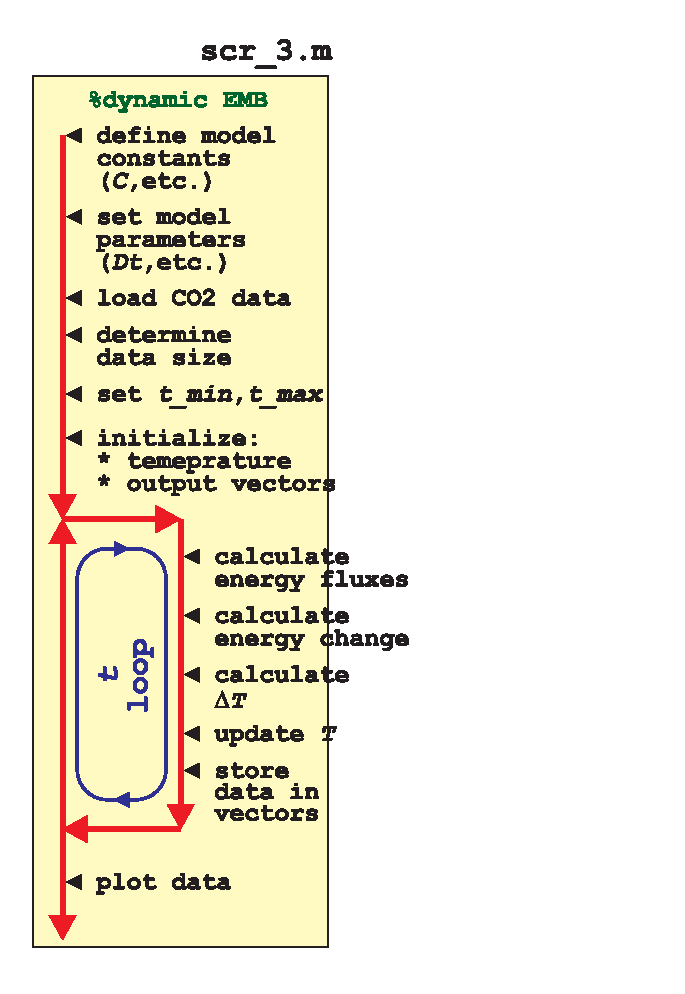
\includegraphics[width=\linewidth]{ch9-schematic-scr3.eps}
\caption{Schematic of the dynamic EBM driven by a history of CO2 (read in from a file).}
\label{fig:ch9-schematic-scr3}
\end{marginfigure}

\begin{enumerate}[noitemsep]
\setlength{\itemindent}{.2in}
\item Add in code to load in the CO\(_{2}\) dataset. You are going to use the  ice-core derived record from week \#1
\\(\texttt{etheridge\_etal\_1996.txt}).
\item From the resulting data array -- determine the minimum and maximum years and the total length (number of rows) of the data. All these values might usefully be stored in variables in your code.
\item Create results vectors of the same length. Create one vector for each of: year, CO\(_{2}\) value, temperature. (Create a single, 3-column array instead if you prefer.)
\item Edit the time loop such that it runs from the minimum to maximum year (with a time-step of 1 year).
\item Also in the loop -- save the current year, \(CO_{2}\) value, and associated calculated temperature.
\end{enumerate}
Be careful that indexing of arrays in \textbf{MATLAB} (for accessing the \(CO_{2}\) value, or saving data to the appropriate row in the vector or array) -- \textbf{MATLAB} \uline{always} starts at a value of \(1\). You will either need to derive an index from the current year\sidenote[][-0.0in]{e.g. current year minus start year plus one.}, or add a loop counter (it is simple to do the former and it takes less lines of code).

When you have this working you should get something like Figure \ref{fig:ch4-ebm-model3} (but note that this was done with not quite the same CO\(_{2}\) dataset ...). If you want to be fancy  you can add a horizontal line indicating the pre-industrial equilibrium solution (using \docenv{line}).

\begin{marginfigure}[-0.0in]
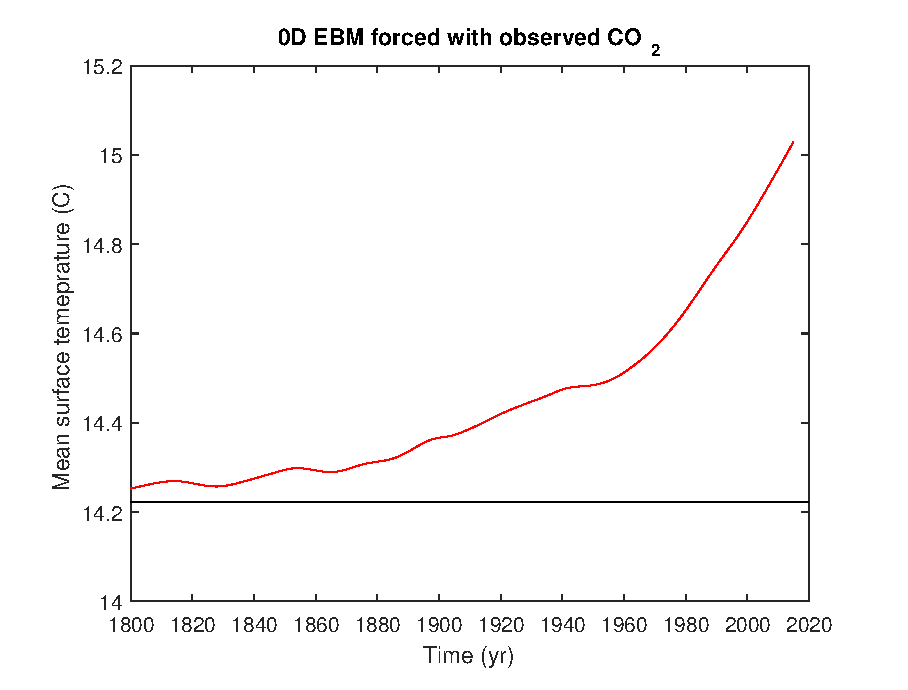
\includegraphics[width=\linewidth]{ch4-ebm-model3.eps}
\caption{Transient EBM response to observed changes in atmospheric CO2. For reference, the pre-industrial equilibrium global temperature is shown as a horizontal black line.}
\label{fig:ch4-ebm-model3}
\end{marginfigure}

Finally, the lagged behavior of the climate system (as encapsulated in your EBM) is maybe not obvious as the forcing (\(CO_{2}\)) is varying. Common in model experiments and characterization, is to create artificial and deliberately simplified forcings and perturbations, so as to more readily diagnose the response time and characteristics of a system. Crete an artificial \(CO_{2}\) data-set, spanning the same time interval as the real data, and at the same frequency, but substitute an idealized \(CO_{2}\) forcing in which \(CO_{2}\) stays constant (at 278 ppm) up until year 1999, then at year 2000, increases to 400 ppm, and stays there. The result of such an experiment should look like Figure \ref{fig:ch4-ebm-model4}.
 
\begin{marginfigure}[-0.0in]
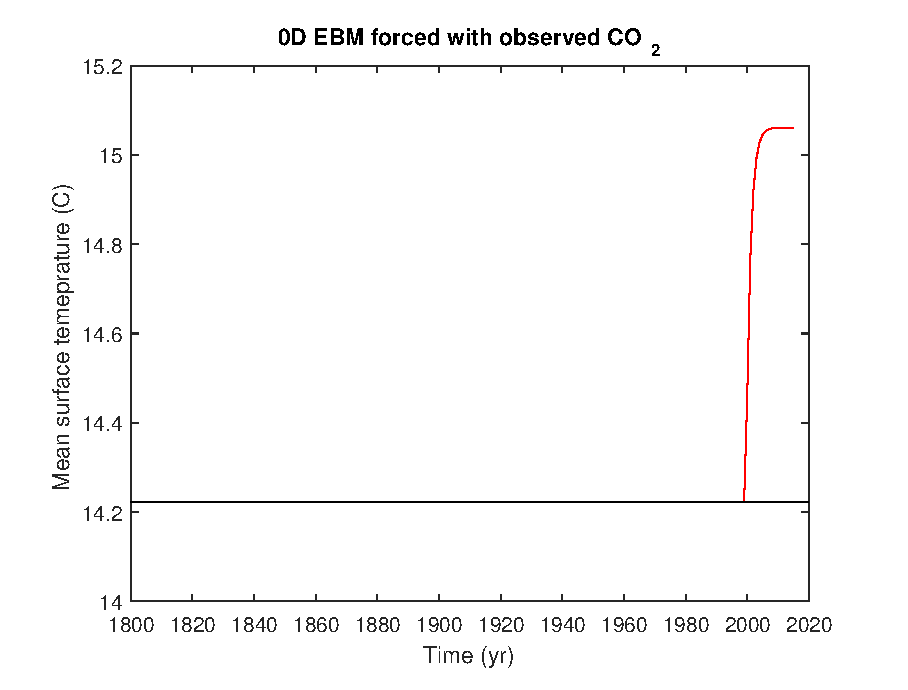
\includegraphics[width=\linewidth]{ch4-ebm-model4.eps}
\caption{Transient EBM response to (fake) changes in atmospheric CO2.}
\label{fig:ch4-ebm-model4}
\end{marginfigure}

Other common model scenarios are linear ramps (up, and/or down) and compound increases, such as a 1\%  per year increase in the concentration of CO\(_{2}\) (each and every year) starting ca. 1960.

%------------------------------------------------

\vspace{1mm}
\noindent\rule{4cm}{0.5pt}
\vspace{2mm}

\noindent To quantify the impact of the ocean heat reservoir on the transient climate response -- try modifying one of your original equilibrium EBM function such that rather than a value of \(S_{0}\), you instead pass in the \(CO_{2}\) concentration. You'll need to add in the \(CO_{2}\) radiative term to the energy balance equation (see earlier Box on \(CO_{2}\) radiative forcing) as you solve for \(T\). Take (and rename) the dynamic EBM script (\texttt{scr\_3}), and in place of the lines of code in the loop that calculated the radiative imbalance and then updated the global surface temperature -- simply call your modified EBM function.

The aim here is to be able to run the same experiment of changing \(CO_{2}\), but with the assumption that the climate is always in equilibrium. Compare the equilibrium vs. dynamic model results (giving an estimation of the importance of the non zero heat capacity of the planet in creating a  lag in temperature in response to a forcing).


%------------------------------------------------

\vspace{1mm}
\noindent\rule{4cm}{0.5pt}
\vspace{2mm}

\noindent A further refinement would be to add a deep ocean heat reservoir (with e.g. diffusive exchange between deep and surface (mixed layer) boxes).

%----------------------------------------------------------------------------------------
% CHAPTER 8
%----------------------------------------------------------------------------------------

\chapter{Numerical modelling -- To infinity (1D) and beyond(!)}
\label{ch:08}

%------------------------------------------------

\newpage

%------------------------------------------------

\section{1-D energy-balance climate model}

Although the Earth is, of course, fundamentally three-dimensional, there are many situations in Earth, Ocean, and Atmospheric sciences when an environmental system can be approximated with a model having just one single (length) dimension. For instance, the structure (e.g. temperature properties) of the atmosphere generally varies vertically much more quickly in distance than it does in the horizontal. Similarly, the changes in the physical, biological, and chemical properties of the ocean are generally much more pronounced with a change in depth rather than for the same distance in latitude or longitude. Because the horizontal gradients in environmental properties in such systems are often relatively small, the horizontal fluxes and exchanges of matter and energy will also be small, particularly compared to vertical transport. The behaviour of some processes which are in reality are operating in a three-dimensional system world can therefore often be usefully analysed by considering their behaviour in just one dimension.

\noindent\rule[0.0ex]{0.5\linewidth}{0.5pt}

\newthought{The simplest possible\sidenote{:o)} example}\marginnote[-0.0in]{\textbf{EXAMPLE OVERVIEW: \begin{enumerate}[noitemsep]
\item Define model grid (latitudes)
\item Calculate zonal surface area
\item Calculate zonal cross-sectional area
\item Calculate incident solar radiation
\item Set up plotting as a function of latitude
\end{enumerate}
}} of a 1-D model is to build on the (zero-D) EBM from before. Well ... perhaps not the simplest, but relatively fun. If you like that sort of thing ...

The idea is: rather than to treat the entire Earth  as a single homogeneous surface characterized by a single surface temperature (and hence single value of outgoing radiation flux), you are going to split the Earths surface up into latitudinal bands. Why latitude and not longitude? Simple inspection of global temperature distributions indicate that the meridional\sidenote{According to the mighty Wikipedia: "along a meridian" or "in the north-south direction".} gradients are much more pronounced that the zonal\sidenote{"along a latitude circle" or "in the west-east direction"} gradients. Obviously, a model would be improved by resolving both meridional and zonal gradients and energy flows, but if you are going to simplify a climate model to just a single dimension, picking latitude seems as good a way to go any any. You can also think in terms of how incoming solar radiation changes most -- ignoring day-night changes as the Earth rotates -- low vs. high latitude regions have the greatest contrast in incoming energy (and hence temperature), and one might suspect that flow of (heat) energy from the Equator towards the poles might be about the single most important transport in the climate system.

We can make a further approximation by noting that the input of solar radiation is roughly symmetrical about the Equator (and assuming that we are going to consider only an annual average climate state of the Earth).\sidenote[][-01.0in]{The actual distribution of the continents on Earth together with how the ocean then circulates on a large-scale completely ruins in this assumption practice, or rather: should a particular degree of 'realism' be required.}\sidenote[][-0.0in]{Because of the (non-zero) obliquity of the Earth, there is a slightly imbalance in the annual averaged solar radiation received by each hemisphere -- dictated by which hemisphere is in its summer when the Earth is closest to the Sun.} So, for this exercise, you need actually only model one hemisphere (and assume that the other one acts identically and that the resulting temperature distribution can be copied/mirrored).

\marginnote[-0.0in]{\begin{mdframed}[backgroundcolor=light-blue, roundcorner=10pt,leftmargin=1, rightmargin=1, innerleftmargin=5, innerrightmargin=5, innertopmargin=5,innerbottommargin=5, outerlinewidth=1, linecolor=light-gray]
\textbf{\#1 Zonal area of the Earths surface}
\\The area of a zonal band of the Earth surface, from latitude \(\phi_{1}\) to \(\phi_{2}\) (in radians), can be found by integrating the circumference of a circle: \(2\cdot\pi\cdot r\), where \(r = r_{0}\cdot cos(\phi)\)
and \(r_{0}\) is the radius of the Earth:
\vspace{2mm}
\\\(\sum_{\phi_{1}}^{\phi_{2}} 2\cdot\pi\cdot r_{0} \cdot cos(\phi)\cdot\delta x\)
\vspace{2mm}
\\\noindent and where \(\delta x\) is an increment in length tangential to the surface equal to \(r_{0}\cdot sin(\delta\phi)\) and which for small \(\delta\phi\) as can be written as \(r_{0}\cdot \delta\phi\).\\ In the limit \(\delta\phi\rightarrow0\):
\vspace{2mm}
\\\(\int_{\phi_{1}}^{\phi_{2}} 2\cdot\pi\cdot r_{0}^{2} \cdot cos(\phi) \;d\phi\)
\vspace{2mm}
\\The zonal area between latitude \(\phi_{1}\) and \(\phi_{2}\) is thus:
\vspace{2mm}
\\\(2\cdot\pi\cdot r_{0}^{2} \cdot (sin(\phi_{2}) - sin(\phi_{1}))\)
\vspace{2mm}
\\\noindent and which is why when you integrate from -90\degree to +90\degree (or -\(\pi/2\) to +\(\pi/2\)) you recover the surface area of a sphere: \(4\cdot\pi\cdot r^{2}_{0}\).
\end{mdframed}}

OK -- so the first step is to divide up the Earth (or one hemisphere), into bands, with each band being subject to the same energy budget as before, including an ocean-dominated heat capacity component, and which will lead to each band having its own characteristic temperature. (Assume for now that each latitude band is characterized by the same fraction of ocean and mean mixed-layer depth.) You can chose how many bands to make. Actually, if you do it the 'easy' way it will not matter how many you want\sidenote{Within reason, but ... as you'll find later, there is a numerical stability penalty to having too many (but simply requiring a shorter time-step to fix.)} and which, as you might have guessed, uses loops. The hard way is to write out all the equations explicitly\sidenote{If you are unsure how a loop is going to pan out in terms of updating the fluxes and calculating the temperature of each zonal band, maybe write out the equations in full initially (for one hemisphere), e.g. for 3 bands: 0-30\degree  N, 30-60\degree N., and 60-90\degree N.}. 

You are going to do construct something like this:
\begin{docspec}
for n = 1:n\_max
\\ \ \ \% CODE GOES HERE
\\end
\end{docspec}
where \texttt{n\_max = 90.0/dlat} and \texttt{dlat} is the width of each band\sidenote[][+0.25in]{
If you loop in \(n\) (latitudinal bands), you can pre-define the northern and southern edge of each band for convenience, and then simply by indexing the appropriate array with \(n\), recover the latitude, e.g.
\begin{docspecmargin}
\% define model grid -- N edge
\\grid\_n = [dlat:dlat:90]; 
\\\% define model grid -- S edge
\\grid\_s = [0:dlat:90-dlat];
\end{docspecmargin}
\noindent where \texttt{dlat} is the increment in latitude between bands.
}.

For each band, it would be nice to write exactly the same equations as before. Except ... you can't. Why? (Hint: spheres have curved surfaces -- who would have guessed? And the surface gets more oblique with respect to incoming radiation as the latitude increases, meaning that the same (per unit area) solar flux is spread over an increasing area.)

\begin{itemize}[noitemsep]
\item For outgoing radiation / energy loss, you need to know the surface area of each band, assuming that each band occupies an equal number of degrees of latitude, and how this varies with latitude. A small hint can be found in  Box \#1. Or the Internet will, as usual, know it all.
\item For incoming solar radiation, you need the cross-sectional area of a band on a sphere.



The original mean incident solar energy per unit area was \(S_{0}/4\) on the basis that the total received radiation was \(\pi\cdot r^{2}_0\cdot S_{0}\) spread over (i.e. divided by) a total surface area of \(4\cdot \pi\cdot r^{2}_0\). You already have the total surface area of a zonal band around the Earth (Box \#1) which you need for calculating the long-wave energy loss from, but now you need the area perpendicular to the incoming solar radiation (i.e. the cross-sectional area). The area of a complete disk is \(\pi\cdot r^{2}_0\) and to cut a long story short ... and  see Box \#2\ ...
the area of a portion of a disk, is:
\vspace{1mm}
\\\(A = \frac{r^{2}_{0}}{2}\cdot(-2\cdot\phi_{1}+2\cdot\phi_{2}-sin(2\cdot \phi_{1})+sin(2\cdot \phi_{2}))\)
\vspace{1mm}
\\\noindent which is *so* much less fun than before :( 
\end{itemize}
Actually, both equations are so little fun, that, assuming that you defined vectors to hold the northern and southern edges of the zonal bands (see later), I'll give you the necessary code fragment for free:
\begin{docspec}    
\% calculate zonal surface area (units radius)
\\loc\_sa = 2.0*pi*( ...
\\ \ \ ( sin(pi*grid\_n(n)/180)-sin(pi*grid\_s(n)/180) ...
\\ \ \  );
\\\% calculate cross-sectional area
\\loc\_ca = 0.5*( ...
\\ \ \ - 2.0*pi*grid\_s(n)/180 + 2.0*pi*grid\_n(n)/180 - ...
\\ \ \ \ sin(2.0*pi*grid\_s(n)/180) + sin(2.0*pi*grid\_n(n)/180) ...
\\ \ \ \ );
\end{docspec}
\noindent where \texttt{loc\_sa} is the surface area of the zonal band, and \texttt{loc\_ca} is the cross-sectional area (\texttt{grid\_n} and \texttt{grid\_s} hold the northern and southern edges, respectively, of the zonal bands).

\marginnote[-2.75in]{\begin{mdframed}[backgroundcolor=light-blue, roundcorner=10pt,leftmargin=1, rightmargin=1, innerleftmargin=5, innerrightmargin=5, innertopmargin=5,innerbottommargin=5, outerlinewidth=1, linecolor=light-gray]
\textbf{\#2 Zonal cross-sectional area}
\\The cross-sectional area of a zonal band ... is a pig to calculate. You start with the area of a circle bordered by a cord, which can be thought of as a line of latitude. This itself, is derived by calculating the area of a segment and subtracting a triangle ... no seriously. I wish I could be bothered to draw you a picture. Google is full of hits for a circular segment.
\\Inconveniently, this is written in terms of the angle of the segment, \(\psi\):
\vspace{2mm}
\\\(A = \frac{r^{2}_{0}}{2}\cdot(\psi-sin(\psi))\)
\vspace{2mm}
\\\noindent Again, you need a picture. If we re-write \(\psi\) in terms of latitude \(\phi\):
\vspace{2mm}
\\\(\phi=\frac{(\pi-\psi)}{2}\)
\vspace{2mm}
\\\noindent then we can reduce this to (recognising, e.g. that \(sin(\pi-2\cdot\phi)\) is simply \(sin(2\cdot\phi)\):
\vspace{2mm}
\\\(A = \frac{r^{2}_{0}}{2}\cdot(\pi-2\cdot\phi-sin(2\cdot\phi))\)
\vspace{2mm}
\\All we need to do then, is to subtract the smaller, high-latitude chord-bounded circular segment from the low-latitude one. Simples.
\end{mdframed}}
 
Obviously(!) you ratio \texttt{loc\_ca} by \texttt{loc\_sa} to get out the relative change in solar flux for that latitudinal zone (as you did for a disk/sphere and ended up with \(S_{0}/4\)). Note that \textbf{MATLAB} just hates units of \degree \ for angles -- you need your latitude values, when you calculate the \(sin\) of the southern and northern boundaries of the zonal band, in units of \uline{radians}.

You are going to to be time-stepping through the simulation (as per the previous EBM with a heat reservoir), and your time-stepping loop needs to go outside (around) the latitude band (\(n\)) loop. The '\texttt{code goes here}'\sidenote{
Along the lines of:
\begin{docspecmargin}
\% (1) calculate net radiation imbalance (W m-2)
\\\% (2) update temperature (of ocean mixed layer)
\end{docspecmargin}
\noindent (with the results array having a zonal band number dimension as well as of time).
} is going to be similar to the code as before, for updating the temperature of the surface (equivalent to the temperature of your ocean mixed layer heat reservoir), but obviously you need a vector to store the temperature of each zonal band.

You are ready to go ... or should be. Probably easiest is to adapt your function from before (and save under a different \textsf{m-file} name) and retain the ability to pass in a time-step and also maximum simulation duration. Amazingly, given the cr*ppy unpleasant trigonometry involved, it seems to work(!) -- illustrated in Figure \ref{fig:ch4-ebm-1d}. As ever, if you give it a particularly inappropriate time-step, funky and meaningless things can happen (not shown). 
\begin{marginfigure}[0.0in]
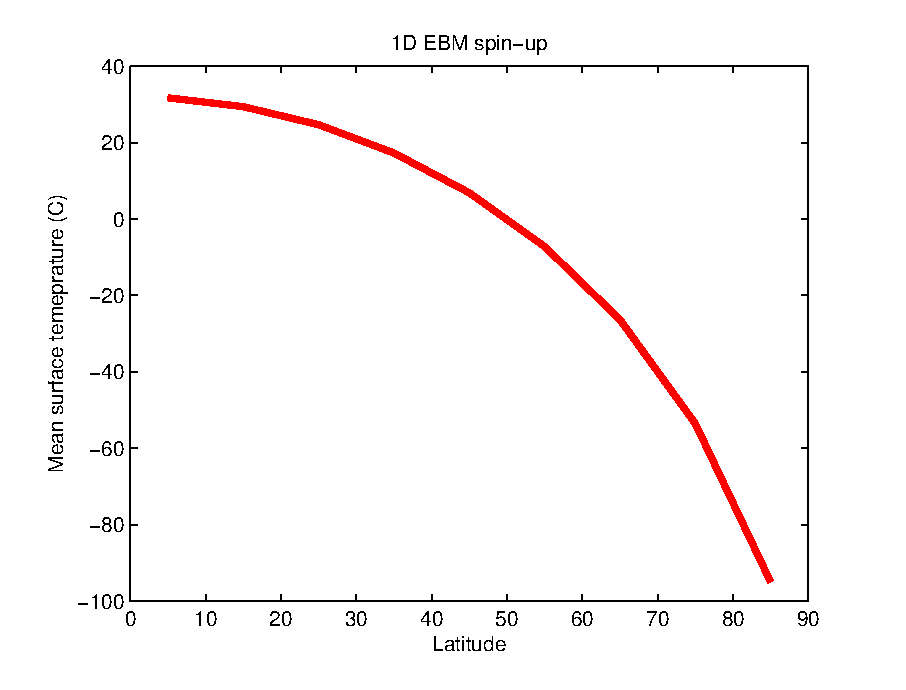
\includegraphics[width=\linewidth]{ch4-ebm-1d.eps}
\caption{Basic 1-D EBM with no latitudinal heat transport and for a single hemisphere only.}
\label{fig:ch4-ebm-1d}
\end{marginfigure}

\vspace{1mm}
\noindent\rule{4cm}{0.5pt}
\vspace{-2mm}

\newthought{In an extension to this Example}, we note that although the distribution of surface temperatures with latitude looks not entirely unreasonable (colder at the poles is good!), you really need data\sidenote{Not the Star Trek, Next Generation, one.} of some sort to be sure the model projection is not bonkers. You had a dataset of annual mean global surface air temperature data before (which you dutifully plotted). You could either eye-ball some numbers from and try and guess appropriate or representative values as a function of latitude and compare to your EBM, or calculate a zonal mean. Actually, \textbf{MATLAB} makes this obscenely simple for you using the \docenv{mean} function\sidenote[][-0.0in]{A function to calculate the arithmetic mean, rather than a nasty and vindictive function.}.

\marginnote{\begin{mdframed}[backgroundcolor=gray!10, roundcorner=10pt,leftmargin=1, rightmargin=1, innerleftmargin=5, innerrightmargin=5, innertopmargin=5,innerbottommargin=5, outerlinewidth=1, linecolor=light-gray]
\docenvdef{mean}
\\\textbf{MATLAB} \texttt{help}, helpfully says:
\begin{docspecmargin}
Average or mean value.
\\S = mean(X) is the mean value of the elements in X
\\if X is a vector.
\\For matrices, S is a row
\\vector containing the mean value of each column.
\end{docspecmargin}
\end{mdframed}}

The only things then to watch out for are:
\begin{enumerate}[noitemsep]
\setlength{\itemindent}{.2in}
\item If the array is in the wrong orientation, you'll find yourself averaging along lines of latitude. This is simple to check as you'll get no noticeable latitudinal gradient in temperature. You should also find in that case that the length of the vector returned by \texttt{mean} matches the longitude grid rather than latitude.
\item Correcting \#1 requires flipping the matrix around with the transpose operator (\texttt{'}).
\item Units -- units of the temperature dataset are K whereas your model is in degrees Centigrade.
\end{enumerate}
\noindent Once you have fixed any obvious data problems, you should end up with something like Figure \ref{fig:ch4-ebm-1d-data1} (January) or Figure \ref{fig:ch4-ebm-1d-data7} (July). Still to be done  is to create an annual average zonal mean from the data that can be contrasted directly with the annual average  EBM output, rather than just a single month of data. Fixing this is left as an exercise for the reader, as they say ...

\begin{marginfigure}[-0.5in]
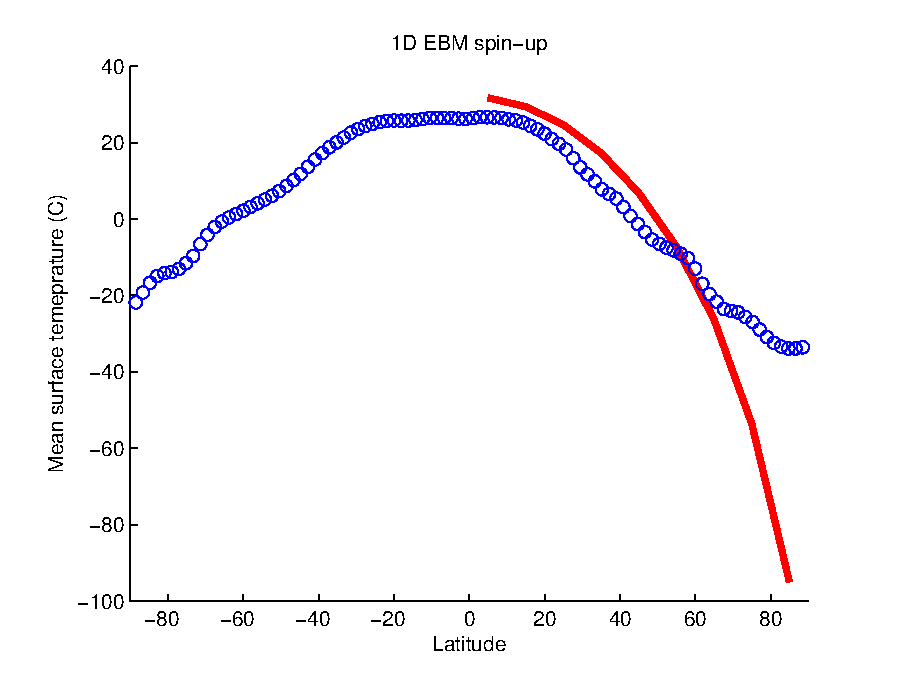
\includegraphics[width=\linewidth]{ch4-ebm-1d-data1.eps}
\caption{Basic 1-D EBM with no latitudinal heat transport (red filled circles). Overlain is the zonal mean observational data for January (blue circles).}
\label{fig:ch4-ebm-1d-data1}
\end{marginfigure}

\begin{marginfigure}[-0.0in]
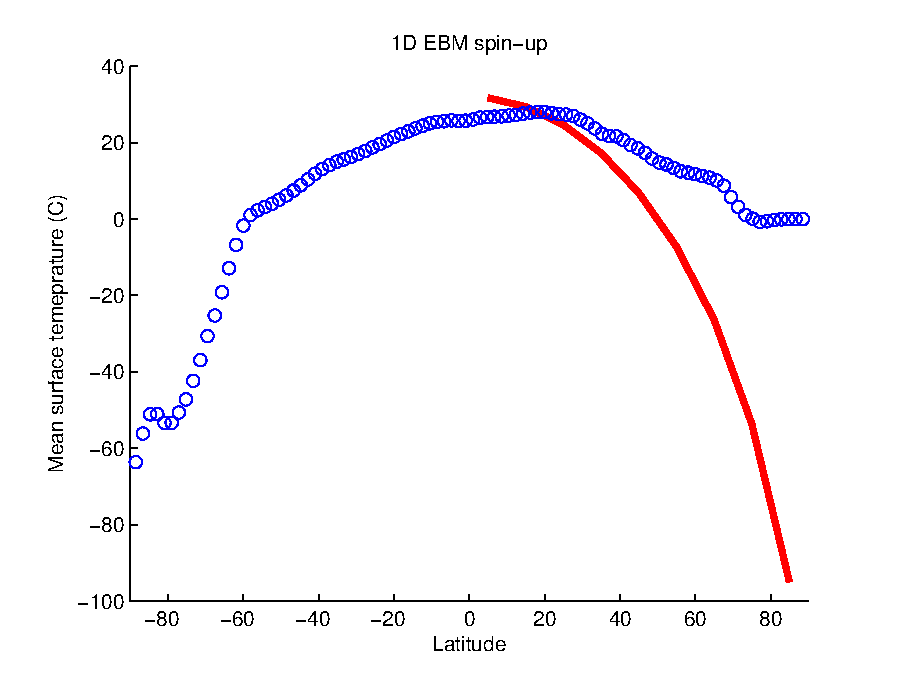
\includegraphics[width=\linewidth]{ch4-ebm-1d-data7.eps}
\caption{As per Figure \ref{fig:ch4-ebm-1d-data1} but for July.}
\label{fig:ch4-ebm-1d-data7}
\end{marginfigure} 

Irrespective of the month (and this might well hold true for the annual mean too), the EBM doesn't exactly provide an ideal fit to the observations. In particular: the North pole is rather too cold and the tropics maybe a little on the warm side. Actually, we are only really looking at half the model-data picture at the moment, and although in the EBM the Southern Hemisphere is a mirror image of the North, it would help to actually see this. So in addition to creating a annual mean zonal temperature profile to plot against the EBM -- also (calculate, or mirror, and) plot the corresponding model projection for the Southern Hemisphere. Something is still missing (in terms of the model accounting for the observations) -- what? Hopefully you correctly guessed (i.e. scientifically and logically deduced) that it is meridional heat transport -- from the (overly) warm tropics to the (too) cold poles.\sidenote{We have also ignored e.g. how surface albedo increases as incident angle decreases -- i.e. solar radiation is generally absorbed more strongly by surface that are perpendicular to the radiation and reflected more efficiently if radiation is glancing at a shallow angle to the surface. However, this would only exacerbate our problem and leave the poles even colder.}

\vspace{1mm}
\noindent\rule{4cm}{0.5pt}
\vspace{-2mm}

\newthought{Extending this Example further},  we'll add some meridional transport of heat energy (to fix the process missing  from the previous version). 

We can encapsulate something of the effect of heat transport along the latitudinal temperature gradient, either by adding a term to represent eddy diffusion and analogous to Fick's law, or by analogy to thermal conductance (albeit with a very poorly conducting atmosphere). They actually both amount to the same thing and will end up with similar looking equations. Taking the thermal conductance approach, the flux of heat energy from one latitudinal band to the next, \(J\) (\(W\)), can be written\sidenote{The equation is conventionally written as negative, assuming the point of reference is the higher temperature, which loses heat energy.}:
\begin{docspec}
\(J = -k\cdot A\cdot \frac{\Delta T}{\Delta z}\)
\end{docspec}
where \(k\) is the thermal conductivity (\(Wm^{-1}K^{-1}\)), \(\Delta T\) is the difference between  the temperatures of two adjacent zonal bands (\(T_{1}-T_{2}\)), and \(\Delta z\) the distance between the bands (measured at the mid-point latitude\sidenote{
Similar to before, if you loop in \(n\) (latitudinal bands), you can pre-define the central latitude of each band for convenience:
\begin{docspecmargin}
\% define model grid mid-point
\\grid\_mid = ... [0+dlat/2:dlat:90-dlat/2]; 
\end{docspecmargin}
although ... this comes in useful only for plotting (e.g. temperatures against the mid-point latitude of the zonal bands, as the separation in latitude is always \texttt{dlat} and hence the separation in distance is always the same(!)).}).\sidenote{This is effectively the same as for the diffusion of CH\(_{4}\) in a soil column in the other 1D modelling example, with the exception of the addition of an explicit area (\(A\)) term here, which we did not worry about before because the model was constructed on a unit area (1 cm\(^{2}\)) basis and hence area did not appear explicitly in the equations.}  

To code this, you simply take the interface area between two adjacent zonal bands (\(A\)), multiplied by \(k\), and by the temperature gradient between the bands (\(\frac{\Delta T}{\Delta z}\)). Heat energy will be lost by the band with the higher temperature, and gained by the adjacent band with the lower temperature, which needs to be taken into account in the energy budget of each band, as summarized below.

The area that heat diffuses across can be simply approximated as the height of the atmosphere over which heat transport takes place, multiplied by the distance around the Earth at that latitude (taking the latitude at the boundary between zonal bands, rather than the mid-point). We'll further assume that for height, the atmosphere can be approximated by equivalent thickness of constant pressure, which would make it  8.5 km (\texttt{8.5E6} m) in height (and then suddenly space beyond that).

\marginnote{\begin{mdframed}[backgroundcolor=gray!30, roundcorner=10pt,leftmargin=1, rightmargin=1, innerleftmargin=5, innerrightmargin=5, innertopmargin=5,innerbottommargin=5, outerlinewidth=1, linecolor=light-gray]
\textbf{Distance between 2 latitudes}
\\Really, you don't need a Box for this. It is embarrassing to make one in fact. But just in case ...
\\The average distance between zonal bands can be estimated from the difference in latitude between the two mid-points of the zones, and divide up the circumference of the Earth proportionally, i.e.
\vspace{1mm}
\\ \(\Delta z=\frac{\Delta lat}{360}\cdot z_{total}\) 
\vspace{1mm}
\\\noindent where \(z_{total}=2\cdot\pi\cdot R\) (the circumference of the Earth at the Equator).
\end{mdframed}}

\marginnote[-0.0in]{\begin{mdframed}[backgroundcolor=gray!30, roundcorner=10pt,leftmargin=1, rightmargin=1, innerleftmargin=5, innerrightmargin=5, innertopmargin=5,innerbottommargin=5, outerlinewidth=1, linecolor=light-gray]
\textbf{Circumference at a specific latitude}
\\This is even more embarrassing to write than the last one. The distance, \(z\), around a particular latitude, \(\phi\) (a Greek character was really not necessary, but it looks way more fancy this way), is:
\vspace{1mm}
\\ \(z=2\cdot \pi\cdot sin(\phi)\cdot R\) 
\vspace{1mm}
\\\noindent (\(sin(\phi)\cdot R\) being the radius of the circle at that latitude).
\end{mdframed}}

Based on the equation -- add a heat diffusion (/conductance) term to your 1D zonal EBM. Note that you do not \textit{a priori} know the value of \(k\). This is not a problem \textit{per se}, indeed, there may be no simple answer or first principals derivation because the processes that govern meridional heat transport in the real atmosphere ... and ocean, may be legion and non-linear. The advantage of a model is that you can find a value of \(k\) that most closely fits the observed data and thus best represents the missing process. Informally, you can simply play with the model and by trial-and-error find a value that seems to fit the observations best.

The key here is to recognise that there are now additional terms  in calculating the energy balance for any particular zone. Whereas previously we could write:
\begin{docspec}
\(\Delta F_{(n)}=F_{solar\_in\:(n)}-F_{longwave\_out\:(n)}\)
\end{docspec}
\noindent now we need:
\begin{docspec}
\(\Delta F_{(n)}=F_{solar\_in\:(n)}-F_{longwave\_out\:(n)}+F_{diffusion\_in\:(n)}-F_{diffusion\_out\:(n)}\)
\end{docspec}

\noindent Note that we have special boundary conditions to consider: the zone bordering the Equator and the zone bordering the pole. This is because the polar zone only gains heat by diffusion from lower latitudes and there is no higher latitude zone than it to diffuse heat to. For the lowest latitude zone, if we are assuming that the Earth is symmetrical about the Equator, then it only loses heat to a higher latitude zone and does not exchange heat energy with the opposite hemisphere (because the temperature is assumed the same).

The structure of your model, within the (outer) time-stepping loop, should then look like:

\begin{enumerate}[noitemsep]
\setlength{\itemindent}{.2in}
\item Loop through all \(n\) latitude bands and calculate the in-coming and out-going radiation.\sidenote[][0.0in]{Don't update any temperatures just yet!}
\item Loop through \((n-1)\) latitude bands (i.e. omitting the highest latitude box, \(n\)), and calculate the diffusion of heat from the band \(n\) to the one adjacent at higher latitude (\(n+1\)). Populate 2 (length \(n\)) vectors -- one to store the diffusive heat gain (presumably from a lower latitude), which will have non-zero values for indices \(2\) through \(n\), and one to store the diffusive heat loss (presumably to a higher latitude), which will have non-zero values for indices \(1\) through \((n-1)\).
\item Loop through all \(n\) latitude bands, calculate the net energy input \(\Delta F_{(n)}\) and update the surface temperature accordingly (based on the heat capacity of the ocean mixed layer and the time-step, as before).
\end{enumerate}

\marginnote[-2.0in]{As before, if you are not entirely confident in what you are doing -- write out the equations long-hand for the simplest possible comparable case -- that of 3 zonal bands: one from 0-30\degree N, one 30-60\degree N, and one from 60-90\degree N. You have two flux calculations in this case -- the transfer of heat energy from the low to the mid latitude box, and from the mid to the high latitude zone. See if you can see the pattern, which will then help you generalize it to \(n\).}

What about the value of \(k\)? You are going to have to guess it to begin with\sidenote[][-0.0in]{If you see nothing plotted, your guess might be too large and you have numerical instability. You could try reducing the time-step. But also start with the lowest conceivable value and work higher.} ... and adjust your guess if the model fits the data worse than before.

As an illustration -- Figure \ref{fig:ch4-ebm-1d-diff0p1} shows the effect of specifying a value of heat conductivity of \(k=0.1\;Wm^{-1}K^{-1}\), while \(k=1.0\;Wm^{-1}K^{-1}\), as shown in Figure \ref{fig:ch4-ebm-1d-diff1p0}, is clearly compete overkill, and much of the pole-to-Equator temperature gradient has been wiped out by over-aggressive heat transport between the bands. (Note that here I have simply mirrored the modelling temperature profile for the Northern hemisphere, to the other (with a \texttt{hold on}). This could have been done much better by combining the vectors and hence obtaining a continuous curve from Souther to North.)

\begin{marginfigure}[-0.0in]
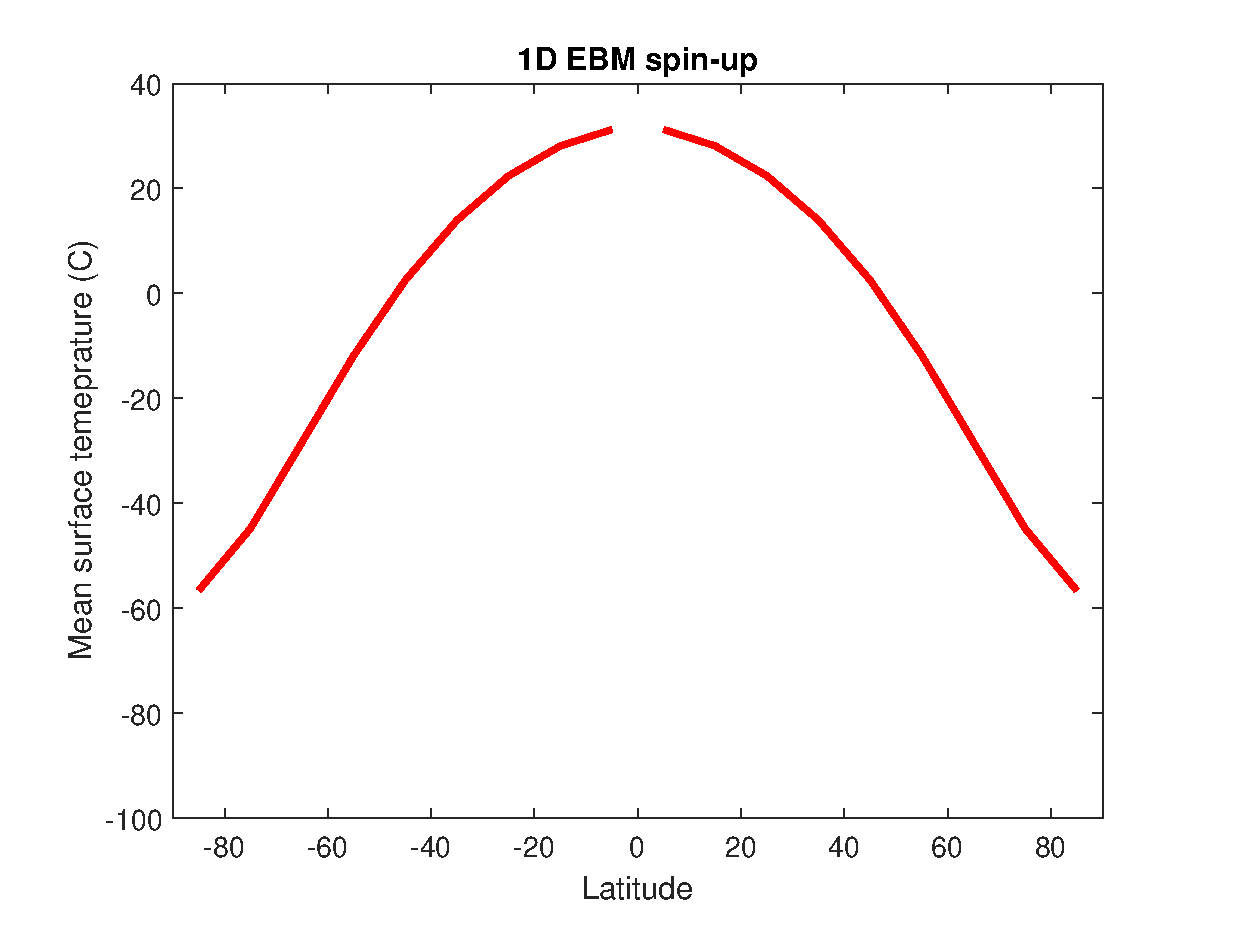
\includegraphics[width=\linewidth]{ch4-ebm-1d-diff0p1.eps}
\caption{1D EBM with an initial guess as to the value of \textit{k}.}
\label{fig:ch4-ebm-1d-diff0p1}
\end{marginfigure}

\begin{marginfigure}[-0.0in]
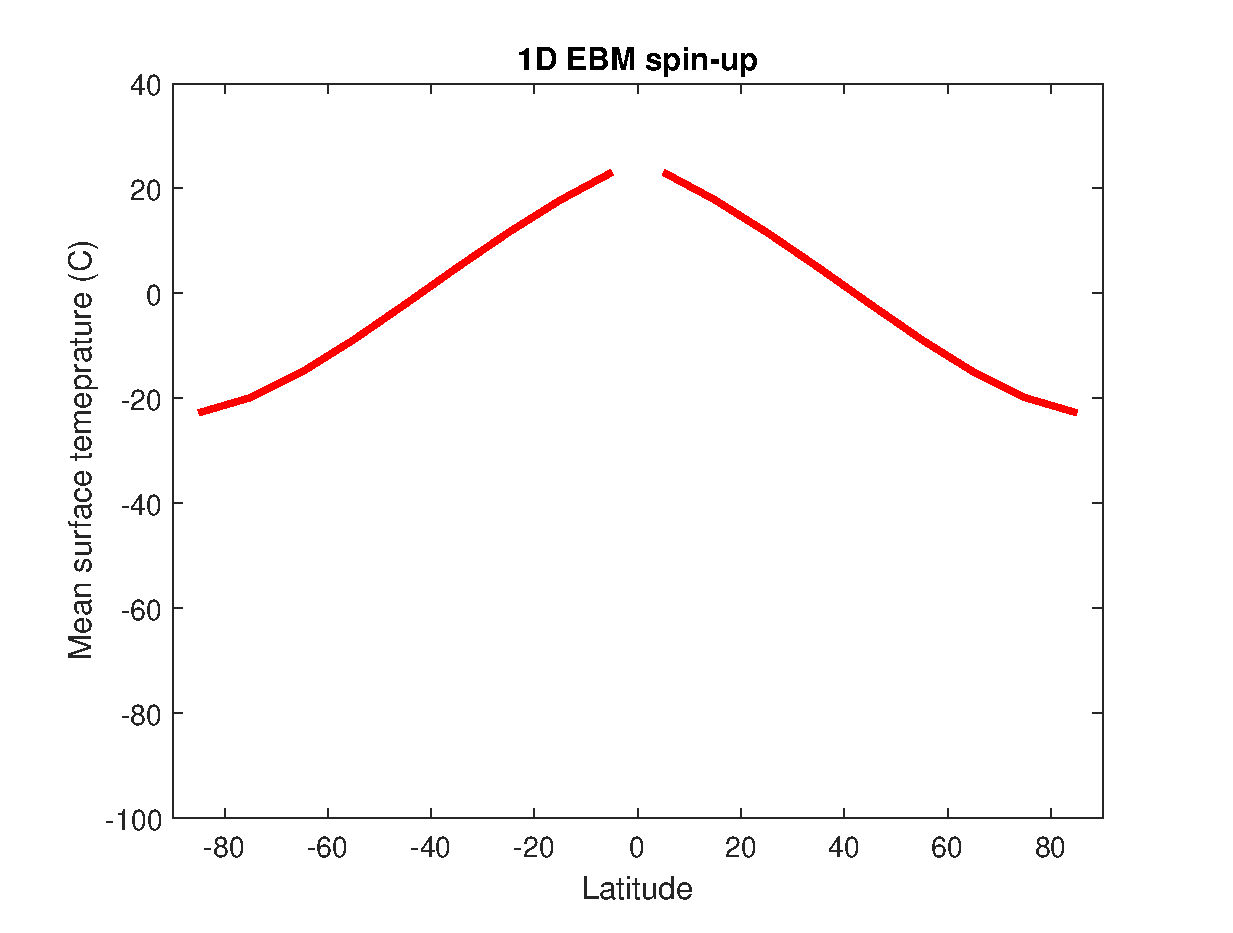
\includegraphics[width=\linewidth]{ch4-ebm-1d-diff1p0.eps}
\caption{1D EBM with a x10 larger value of \textit{k}.}
\label{fig:ch4-ebm-1d-diff1p0}
\end{marginfigure}

%------------------------------------------------

\newpage

%------------------------------------------------

\section{1-D reaction-transport model}

\newthought{A rather scientifically different, but conceptually somewhat similar example}, consider diffusion of a gas through a porous medium. We will take the example of methane (CH\(_{4}\)) diffusion into soils, but there are many other situations in the Earth, Ocean, and Atmospheric sciences where (diffusive) transport in 1-D is critical to understand (such as the supply of solutes to the interface of a growing mineral crystal). 
At its simplest, we have a concentration of CH\(_{4}\) in the atmosphere, which we will assume does not change with time (i.e., the reservoir is in effect infinite). We will call this concentration \(C_{0}\). Because we are not going to allow the value of \(C_{0}\) be affected by whatever happens in our 1-D soil column (we are not concerned in this exercise in any role that the soil methane sink might play in controlling the concentration of CH\(_{4}\) in the atmosphere itself), it is a condition imposed on the model. This is known as a boundary condition (and because it is at the top of the soil column, it is an upper boundary condition).

In the soil we have a population of methane-consuming bacteria ('methanotrophs') who are taking up and metabolizing the CH\(_{4}\) (there will also thus also be a return of CO\(_{2}\), the metabolic product of CH\(_{4}\) oxidation, from the soil to the atmosphere). Because CH\(_{4}\) is being depleted at depth, there will be a gradient in CH\(_{4}\) concentrations along which CH\(_{4}\) there will be net diffusive transport, illustrated in Figure \ref{fig:ch4-soilmodel}. The scientific question is thus; what is the flux of CH\(_{4}\) into  soils? This is important (no, really!) because methane is a powerful greenhouse gas and (aerobic) soils might constitute an important sink of this gas.
\sidenote[][-4.5in]{In reality the system looks more like Figure \ref{fig:ch4-soilmodel2}, and actually, even more like Figure \ref{fig:ch4-soilmodel3} ... adding considerable complexity (and dynamics).}

\begin{marginfigure}[-5.0in]
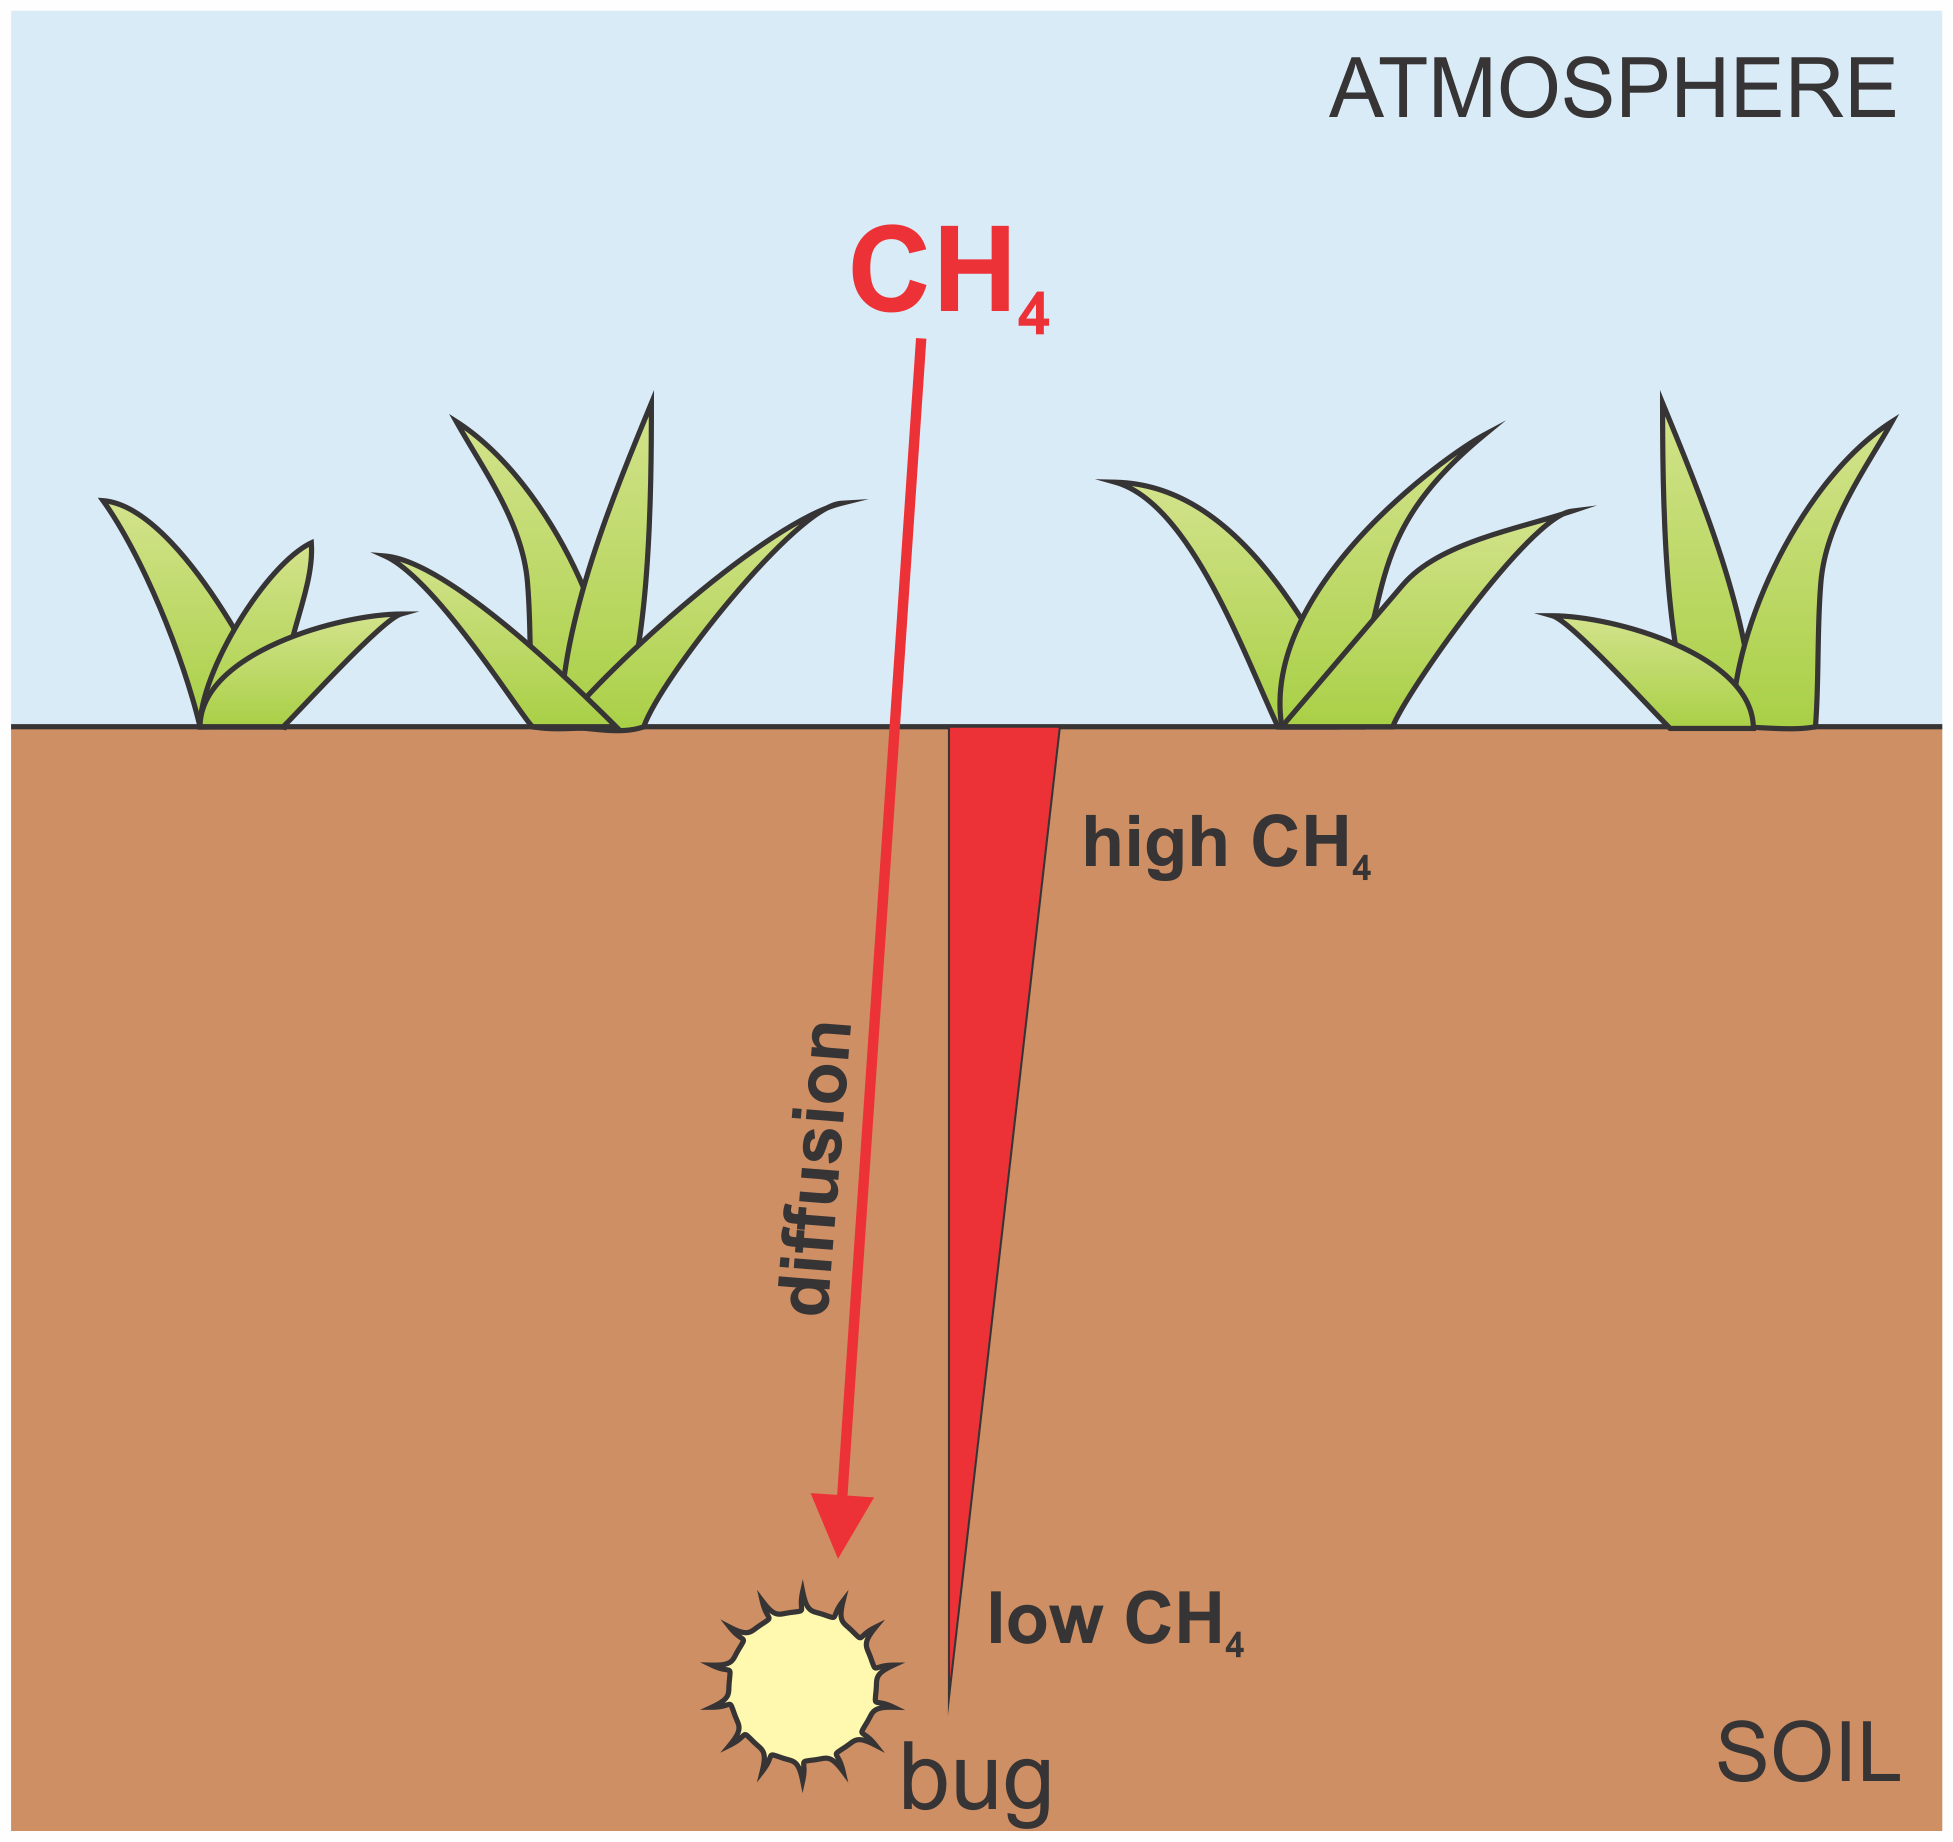
\includegraphics[width=\linewidth]{ch4-soilmodel.png}
\caption{Idealized schematic of the soil-CH4 system.}
\label{fig:ch4-soilmodel}
\end{marginfigure}

\begin{marginfigure}[-1.5in]
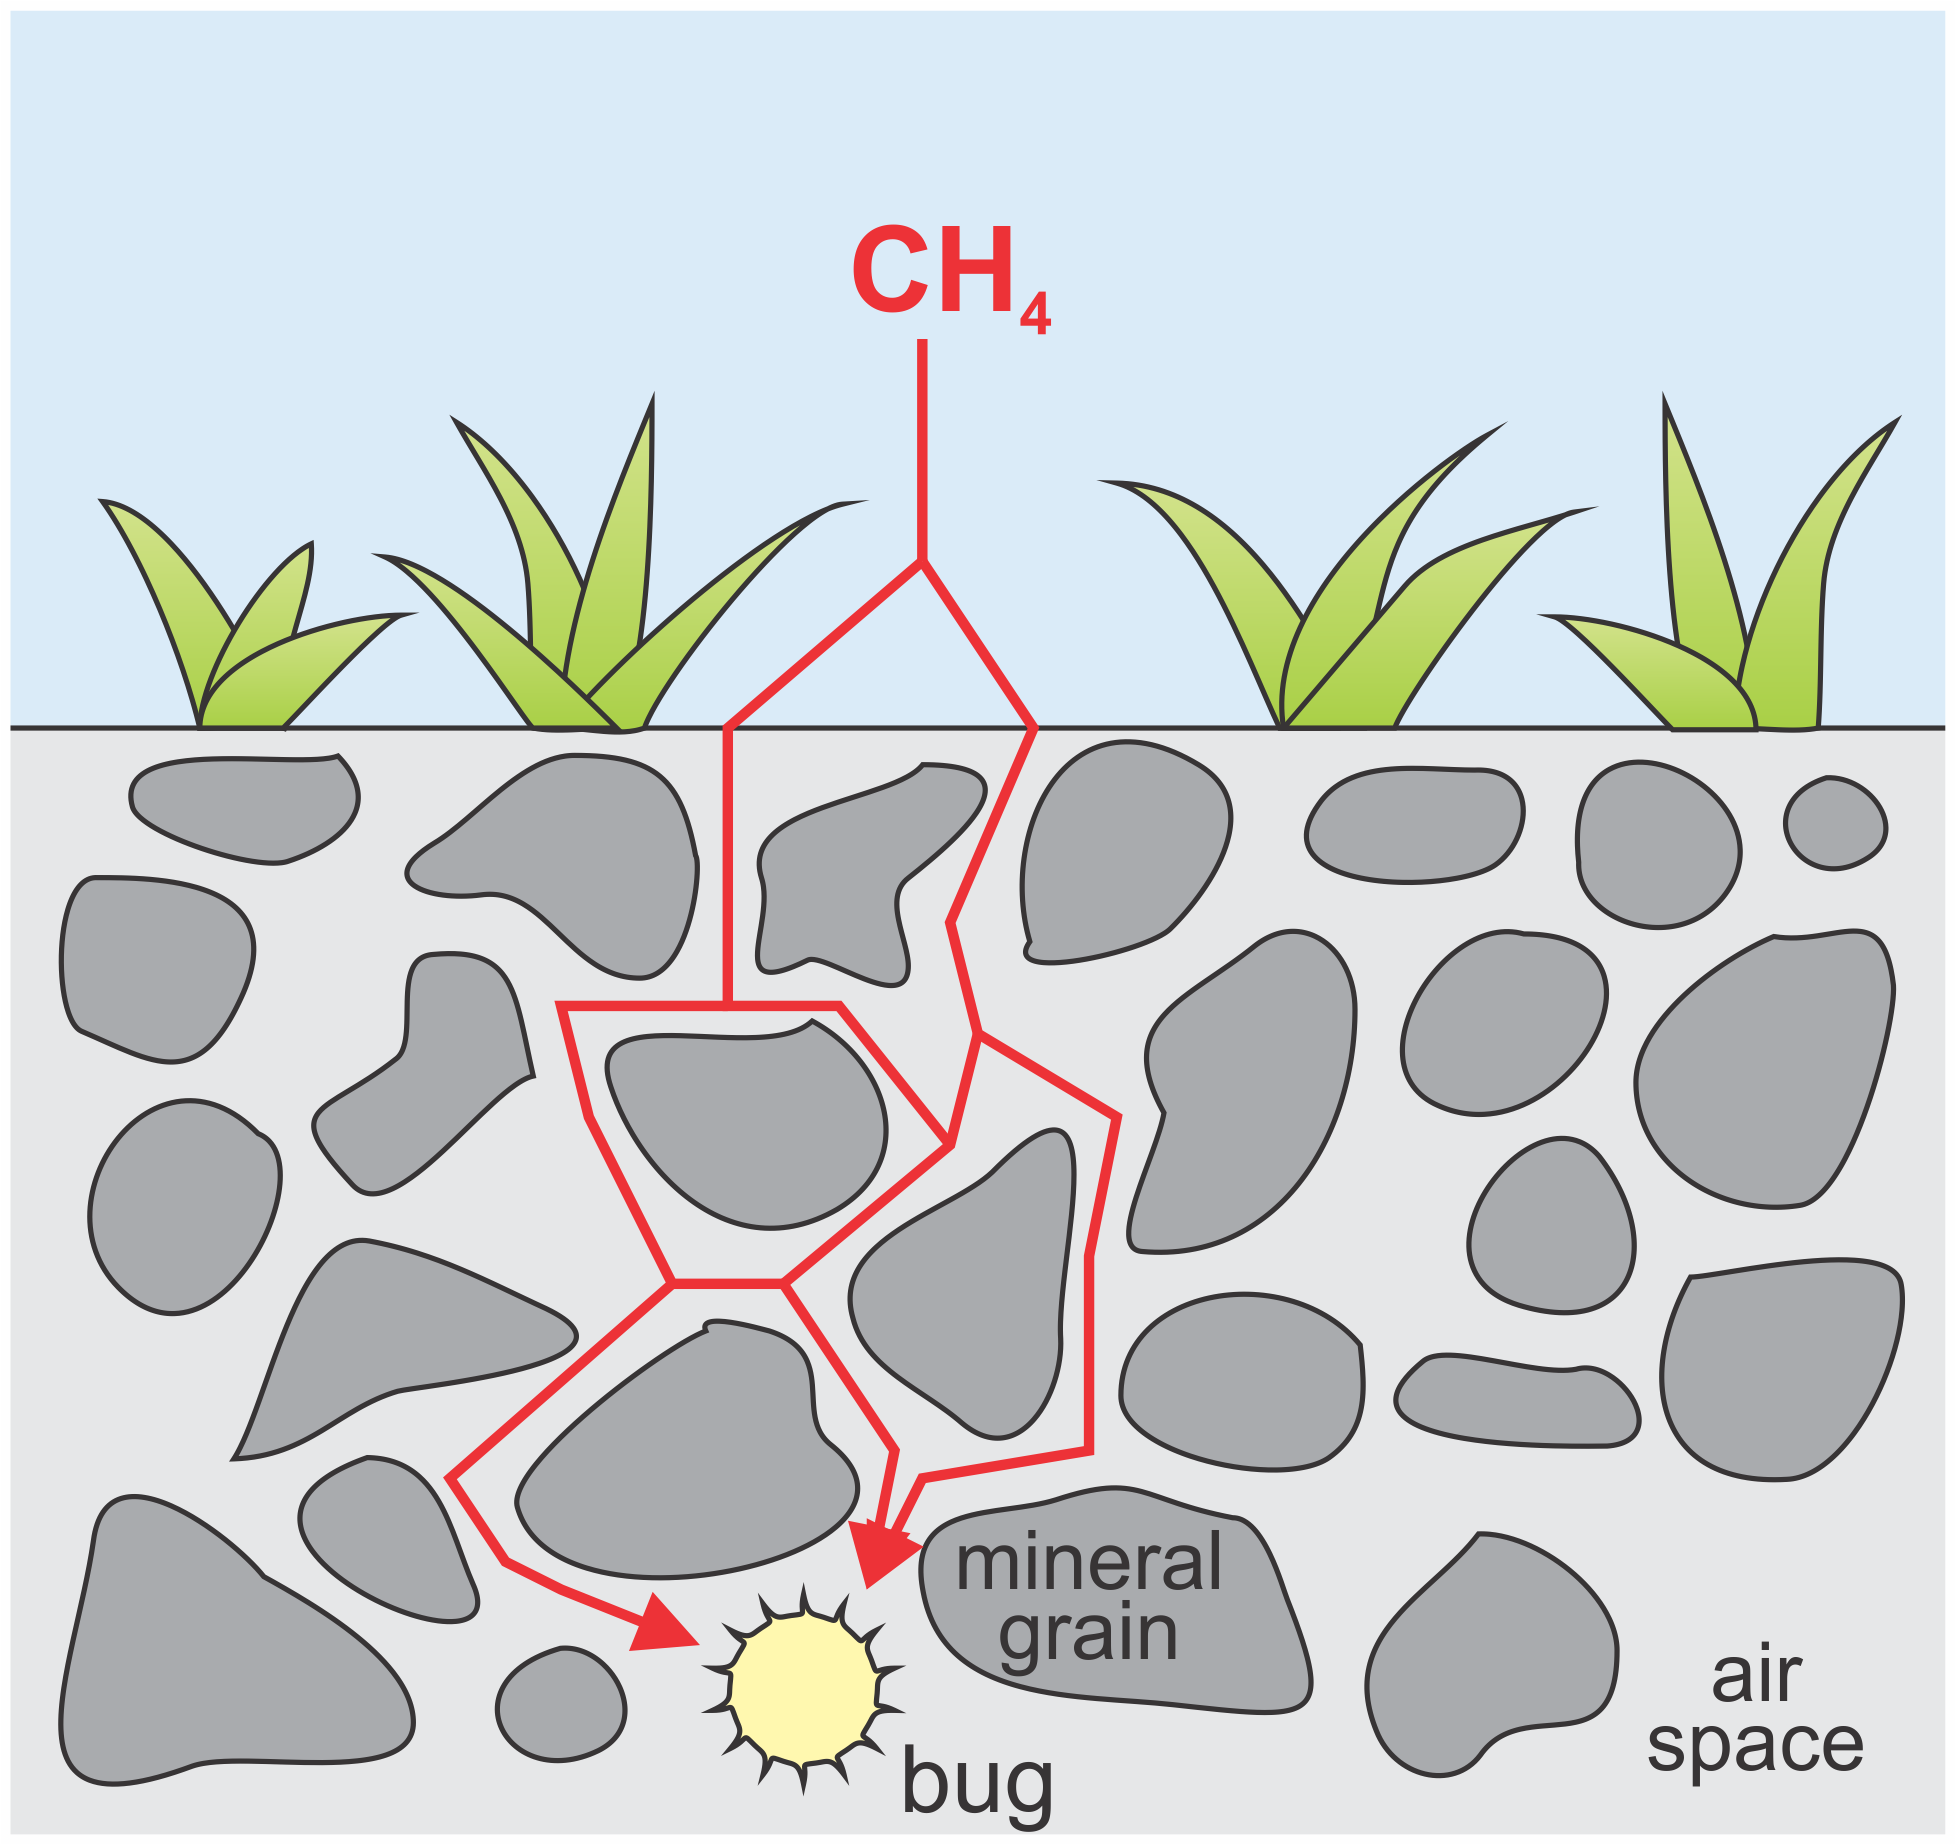
\includegraphics[width=\linewidth]{ch4-soilmodel2.png}
\caption{Slightly less idealized schematic of the soil-CH4 system.}
\label{fig:ch4-soilmodel2}
\end{marginfigure}

\begin{marginfigure}[0.0in]
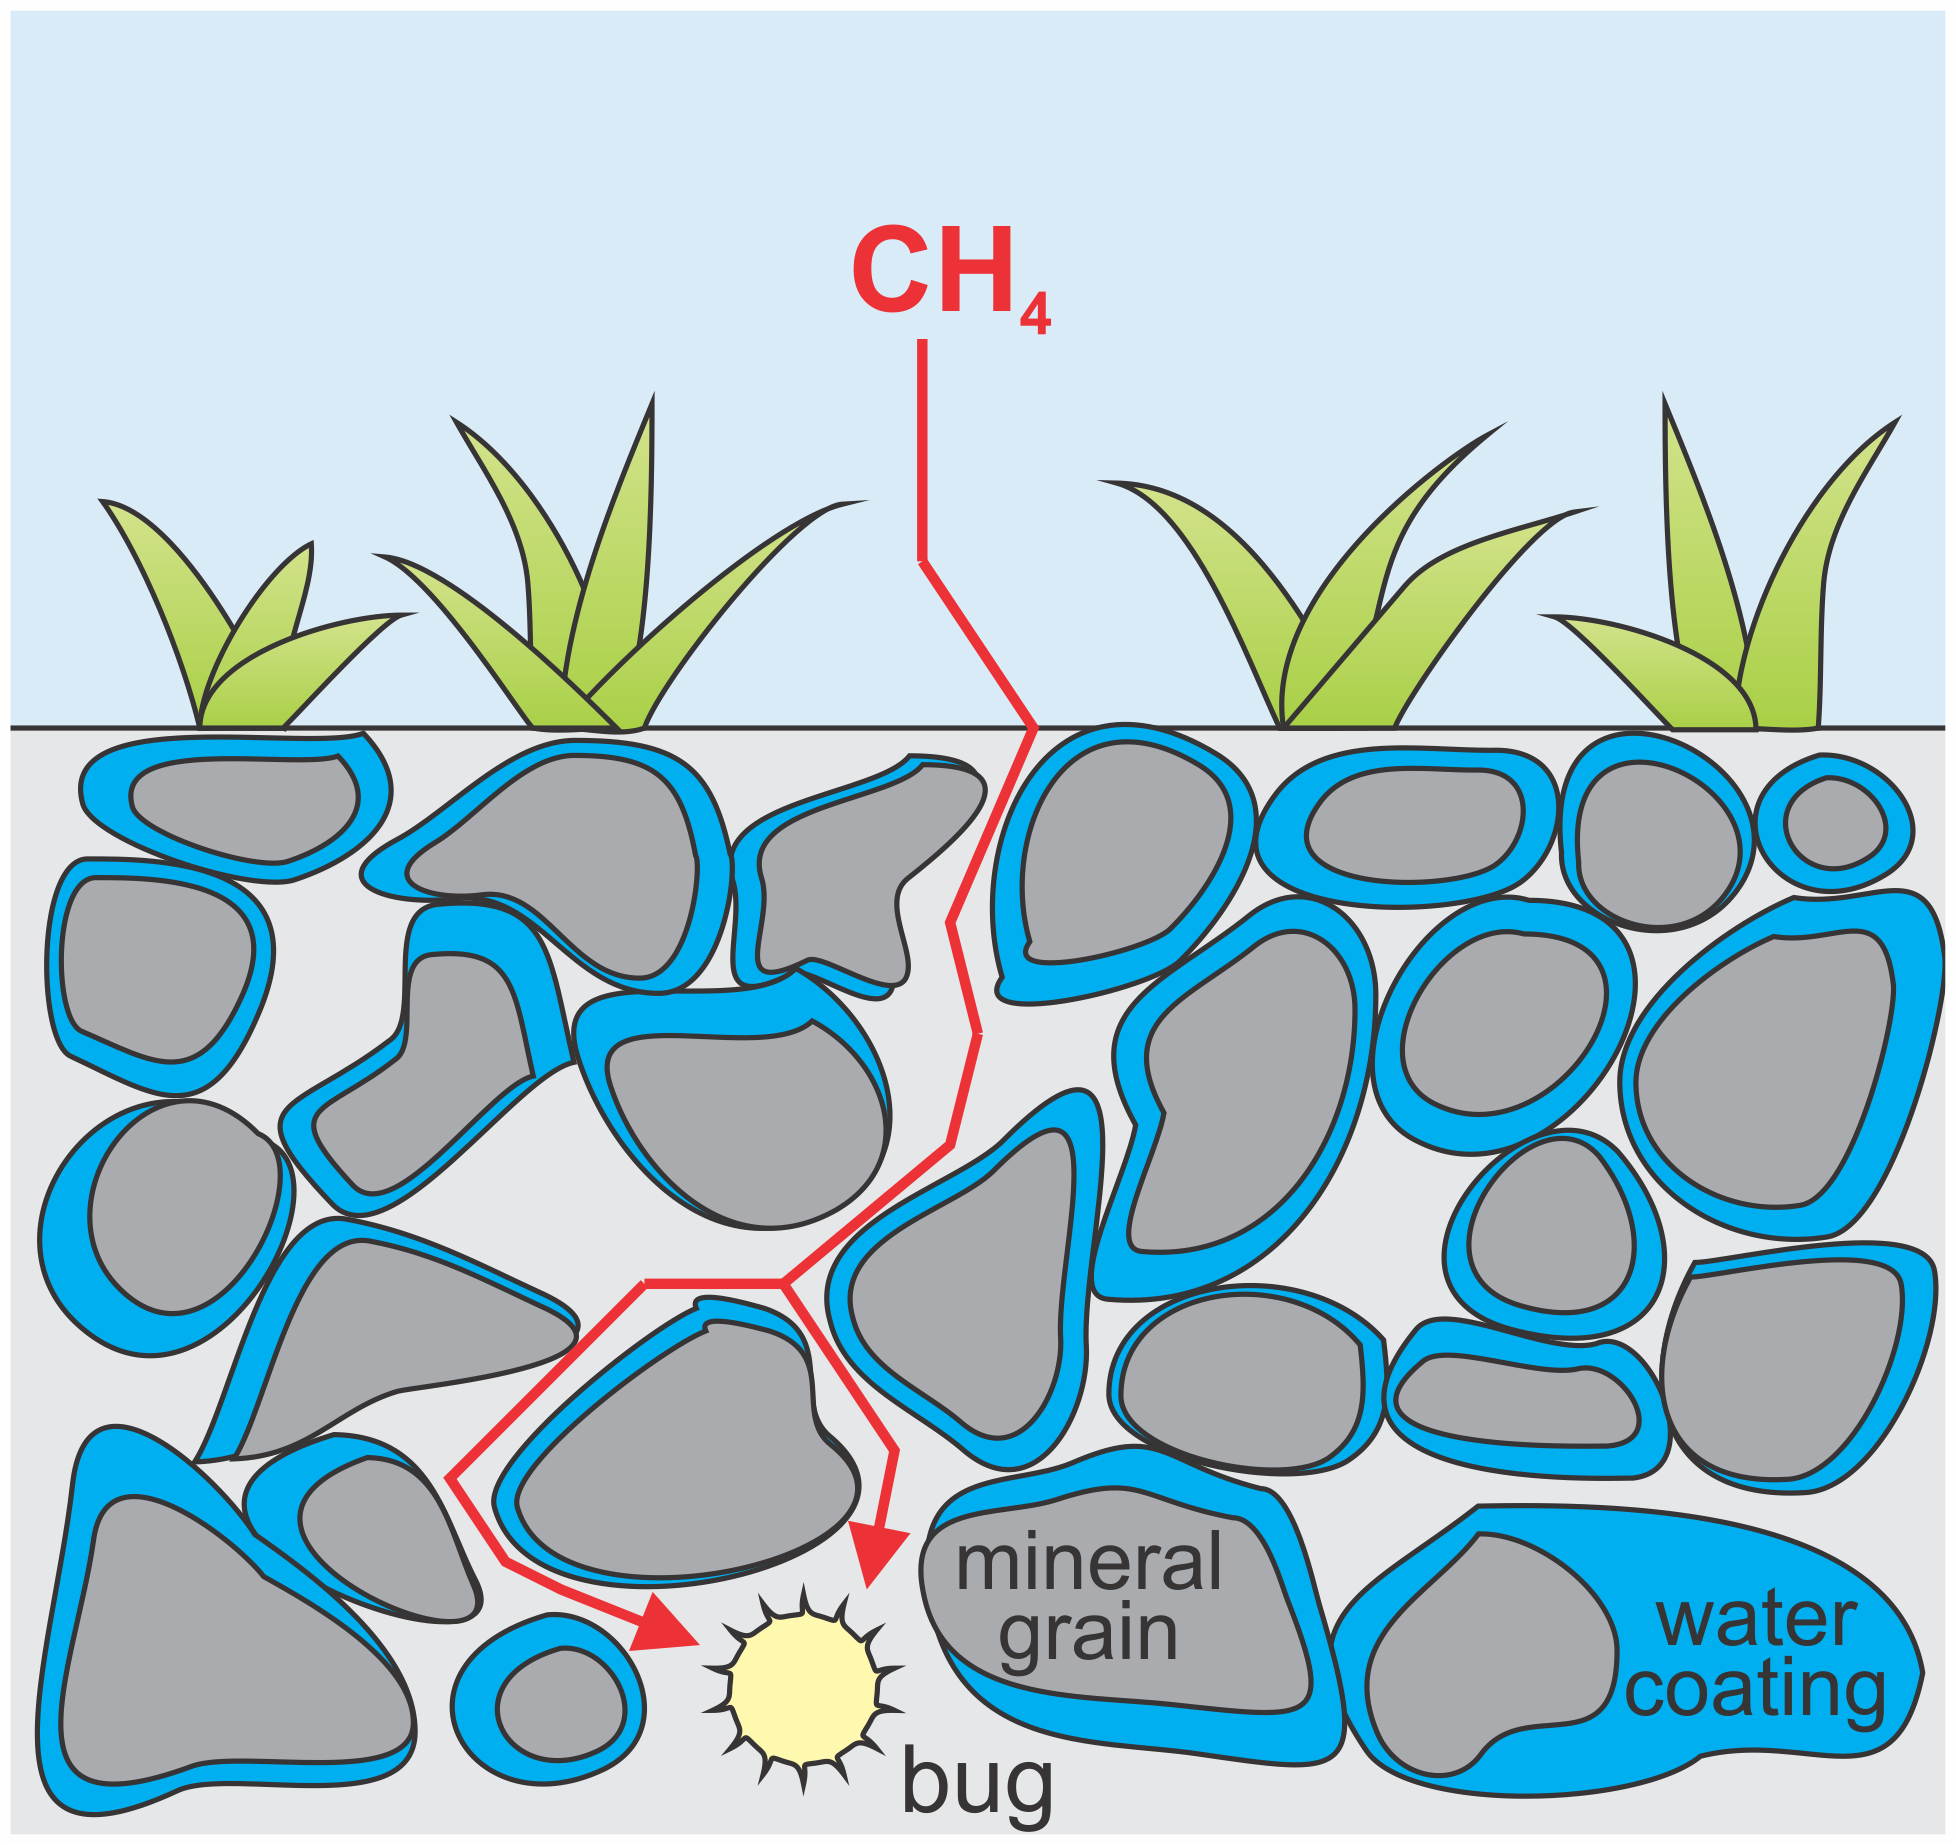
\includegraphics[width=\linewidth]{ch4-soilmodel3.png}
\caption{Even less idealized and almost realistic, schematic of the soil-CH4 system.}
\label{fig:ch4-soilmodel3}
\end{marginfigure}

If all CH\(_{4}\) in the pore space was entirely consumed at some known depth, \(z\), then we would have a gradient of \(C_{0} - 0\) (\(C_{0}\) being the imposed upper boundary condition, and zero being the concentration at depth) in methane concentration, and diffusion would be taking place over a depth \(z\). If \(D\) is the diffusivity of CH\(_{4}\) (in soil), with units of cm\(^{2}\)s\(^{-1}\), then we can easily calculate the initial flux, \(J\), of methane into the soil by Fick's law (as cm\(^{3}\) CH\(_{4}\) per second (s\(^{-1}\)) per unit cross-sectional area (cm\(^{-2}\))):
\begin{docspec}
\(J = D\cdot\frac{C_{0}-0}{z}\)
\end{docspec}
or, more generally we can write that at any point in the soil that the following condition must be satisfied:
\begin{docspec}
\(J = D\cdot\frac{\Delta C}{\Delta z}\)
\end{docspec}
where \(\frac{\Delta C}{\Delta z}\) is the gradient in CH\(_{4}\) concentration (i.e., the change in concentration divided by the change in depth).

If all there was to the soil methane system was consumption to zero at known depth, we could simply use an analytical solution to calculate the CH4 flux into the soil. Unfortunately, life is rarely as kind, and there are a number of complications (see background material). For instance, the bugs do not all live at the same depth in the soil column (although that is the assumption made in \textit{Ridgwell et al.} [1999]), nor have a constant activity throughout the year. Also, soil properties vary with depth, which affects the porosity and tortuosity of the soil (basically, how interconnected soil pore spaces are, and thus in effect how conductive the soil is to gaseous diffusion) and thus the diffusivity (\(D\)) of CH\(_{4}\) in the soil column, illustrated in Figure \ref{fig:ch4-soilmodel2}. We will assume an initial value for \(D\) of 0.186 cm\(^{2}\) s\(^{-1}\).

Because we would quite like a general model for soil CH\(_{4}\) uptake that was capable of accounting for these sorts of complications if necessary, we will solve the system numerically rather than restricting us to a simple analytical solution. This is what we will be doing in this exercise -- constructing the basic model of atmospheric CH\(_{4}\) diffusion into the soil, although there is not time in this exercise to go on and consider the metabolic consumption of atmospheric CH\(_{4}\) by methanotrophic bacteria.

\vspace{1mm}
\noindent\rule{4cm}{0.5pt}
\vspace{2mm}

\marginnote[-0.0in]{\textbf{EXAMPLE OVERVIEW: 
\begin{enumerate}[noitemsep]
\item create function
\item create arrays and initialize model parameters
\item set up plotting (useful for later)
\item create time-stepping loop framework
\item add code to calculate fluxes:
\\(I): flux into surface layer
\\(II): flux into the (9) interior layers in a loop
\item add code to update concentrations based on fluxes:
\\(I): updating of first 9 layer concentrations in a loop
\\(II): updating of bottom-most layer
\end{enumerate}
}}

\noindent If we divide up the soil profile into 10 equally-spaced (equal thickness) layers\sidenote{It need not be 10 -- choosing 10 layers of 1 cm thickness each, just simplifies things.}, the basics of the model will be an array with 10 rows, one (row) location in the array representing the CH\(_{4}\) concentration in the pore space corresponding to each 1 cm thick interval of soil (see Figure 1). Thus, row \#1 corresponds to the concentration in the 0-1 cm depth interval, C1, \#2 corresponds to the 0-1 cm depth interval, C2, ... , and \#10 corresponds to the 9-10 cm depth interval, C10. We will also need to create an array to store the average depth, \(z_{n}\) at which each of the CH\(_{4}\) concentrations is measured. These depths will be; 0.5 (\(z_{1}\)), 1.5 (\(z_{2}\)), 2.5 (\(z_{3}\)), ... , and 9.5 cm (\(z_{10}\)).

We are now ready to calculate the diffusion of CH\(_{4}\) down the soil column. From the earlier equation, you know that you can relate the methane flux to the gradient in the soil, and the gradient between any two successive soil layers is equal to:
\begin{docspec}
\(\frac{C_{n} - C_{n+1}}{z_{n+1} - z_{n}}\)
\end{docspec}
This is just to say, the difference between the concentration in any layer n and the concentration in the layer immediately below it (which will be number \(n+1\)) divided by the depth interval between the mid-points of the same two layers, which is the depth (from the surface) of the deeper layer (\(z_{n+1}\)) minus the depth of the layer immediately above (which is layer \(n\)).

Putting this all together, the downwards flux of CH\(_{4}\) between layers is given by:
\begin{docspec}
\(J = D\cdot\frac{C_{n} - C_{n+1}}{z_{n+1} - z_{n}}\)
\end{docspec}

You can think of this system as analogous to the Great Lake model system\sidenote{Except less wet.}\sidenote{And smaller.}\sidenote{And in the soil ... OK, so not so much like the Great Lakes system ...} -- there we had a series of reservoirs storing stuff (heavy metals), and there was a flow of material from one lake to the next. Here we have gaseous CH\(_{4}\) in soil pore spaces rather than metals in solution in a lake, and we have diffusion of CH\(_{4}\) from one soil level to another rather than a flow of water from one lake to another. The only real difference is that in the Lake Model more of the work was done for you and you were given the flow rates between lakes, whereas here you have to calculate the transport (diffusion) rate of CH\(_{4}\). The strategy for simulating the behavior of this system through time will be very similar though -- stepping through time, and during each time step calculating the mass fluxes of CH\(_{4}\) between layers and adding this to the pre-existing concentrations in each layer. The other difference with the Lake Model is that all the soil layers in an indexed array rather than being given different (lake) names, allowing you to use a loop.

OK -- now for the to-do stuff ...

\begin{enumerate}
\setlength{\itemindent}{.2in}

\item 
Create a new \textbf{m-file} \textit{function}.  Pass in the   run length (in units of seconds) of the model simulation as a parameter, and e.g. call it \texttt{maxtime}. See the  blurb from previously  for how to define a function. If you want to be tidy: add a \texttt{close all} statement near the start of the \textit{function}.\sidenote{Note that because the variables created in a function are \textit{private} (and not seen by the rest of the MATLAB workspace), there is no need to issue a \texttt{clear all}. In fact: if you add a \texttt{clear all} at the start, you'll clear the (run length) variable that you have just passed in ... :(}

\item
Create a 10\(\times\)1 vector array call \texttt{conc} and initialized with all zeros\sidenote{To save time -- use the \textbf{MATLAB} function \texttt{zeros}.}. This is the variable array for storing the concentration of CH\(_4\) in each 1 cm interval of the soil profile. Note that we are assuming no methane is present in the soil to start with (zero soil CH\(_{4}\) concentrations is the initial condition of the model).
\\Also create a 10\(\times\)1 vector array called \texttt{J}, again initialized with all zeros, to store the fluxes of CH\(_{4}\) into each of the 10 soil layers from the one above (analogous to how you had the series of river fluxes associated with the various lakes in a previous exercise).
\\Then create a 10\(\times\)1 vector array \texttt{z\_mid} to store all the soil mid-layer depths (0.5, 1.5, 2.5, ... , 9.5). (This is a parameter array for helping in the plotting of soil CH\(_{4}\) concentration against depth, later on.) Note that you need to create an array of 10 values, starting at 0.5, ending at 9.5, and with a step interval of 1.0. Go dust off the colon operator to create this vector array.
\\Also create a parameter (\texttt{conc\_atm}) to store the concentration of CH\(_{4}\) in the atmosphere. To keep things as simple as possible, you will be assuming units of cm\(^{3}\) cm\(^{-3}\), so that the atmospheric CH\(_{4}\) concentration becomes 1.7\(\times\)10\(^{-6}\) cm\(^{3}\) CH\(_{4}\) cm\(^{-3}\) (equivalent to 1.7 ppm), i.e.,:
\begin{docspec}
conc\_atm = 1.7E-6;
\end{docspec}
Also, just for completeness, define a constant to store the depth at which the soil surface meets the atmosphere:
\begin{docspec}
z\_atm = 0.0;
\end{docspec}
Finally, define a parameter to store the value of the diffusivity constant \(D\) (0.186 cm\(^{2}\) s\(^{-1}\)):
\begin{docspec}
D = 0.186;
\end{docspec}

\item 
Create a basic time stepping loop. Define a time-step length (\texttt{dt}) to take -- this is the amount of time that going around the loop each time represents. Call the time-step length parameter \texttt{dt} and assign it a value of 0.1 (s) (do this somewhere before the loop starts in the \textbf{m-file} but after the function definition line at the very top of the script). The model simulation length you want is given by the (passed) parameter \texttt{maxtime}, and each time around the loop lasts \texttt{dt} in model time, so how many counts around the loop do you need to take ... ? If you call the loop counter \texttt{tstep}, then it should be obvious :o) that the start of the loop will look something like:
\begin{docspec}
for tstep = 1:(maxtime/dt)
\end{docspec}
Yes? Before you do anything else, play with the function and check that the time-stepping loop is working and that you understand what it is doing. Try printing out (\texttt{disp()}\sidenote{The display line(s) should go inside the loop, of course.}) the current loop value of \texttt{tstep} as well as the time elapsed in the model.\sidenote{Equal to the loop count multiplied by the time-step length:
\begin{docspecmargin}
tstep*dt
\end{docspecmargin}
}
One way of displaying what is happening in the loop is to add a debug line such as:
\begin{docspec}
disp(['time-step number = ' num2str(tstep) ', ...
\\time elapsed = ' num2str(tstep*dt) ' seconds']);
\end{docspec}
(All I am doing here is concatenating several strings together -- a description of what is being written out followed by a value (a number variable converted to a string using \texttt{num2str}), then another description of what is being written out followed by a value, and finally the units of the second number.) If your function was called \texttt{ch4model} (for instance) and you type:
\begin{docspec}
>> ch4model(1.0)
\end{docspec}
you should now get something like:
\begin{docspec}
time-step number = 1, time elapsed = 0.1
\\time-step number = 2, time elapsed = 0.2
\\time-step number = 3, time elapsed = 0.3
\\time-step number = 4, time elapsed = 0.4
\\time-step number = 5, time elapsed = 0.5
\\time-step number = 6, time elapsed = 0.6
\\time-step number = 7, time elapsed = 0.7
\\time-step number = 8, time elapsed = 0.8
\\time-step number = 9, time elapsed = 0.9
\\time-step number = 10, time elapsed = 1
\end{docspec}
The loop has gone around 10 times because you asked for 1.0 s worth of model simulation (the passed parameter \texttt{maxtime}) and the time-step (\texttt{dt}) is defined as 0.1 s. Happy? (\texttt{:o)})

\item
Run what you have so far and make sure that it works.\sidenote[][-0.0in]{Note that because the variables in a MATLAB function are private (and are thus not listed in the Workspace window), if you want to check the values in this array you could first leave off the semi-colon from the end of the line so that \textbf{MATLAB} prints the array contents to the screen. Or, explicitly add in a \texttt{disp()} line. Or ... add a breakpoint somewhere in the code and view the variable values when the program pauses.}
\\\uline{Remember}: build up a piece of computer code piece-by-piece, testing at each step before moving on. Believe me, there'll be more time for beers at the end compared to trying to write it all in one go and then not having a clue as to why it is not working ...

\item
At the end of the function (i.e., after the loop has ended), plot the concentration profile of CH\(_{4}\) in the soil column -- you will want depth (cm) on the \textit{y}-axis and concentration on the \textit{x}-axis. Depth should run from 0 cm at the top to 10 cm at the bottom. Scale the \textit{x}-axis so that concentration runs from 0 to 2.0\(\times\)10\(^{-6}\) cm\(^{3}\) cm\(^{-3}\). Also plot on the same graph as a point the atmospheric CH\(_{4}\) concentration at the surface of the soil, whose value is held in the parameter \texttt{conc\_atm}.\sidenote[][0.0in]{\texttt{hold on} and then using the \texttt{scatter} function is probably the easiest way.}\sidenote[][0.0in]{Note that \textbf{MATLAB} does not like you trying to plot the \textit{y}-axis with the numbers getting more negative as you go up the axis. One way around this is to plot the negative of the depth on the y-axis; e.g.:
\begin{docspecmargin}
plot(conc(1:10),-z\_mid(1:10));
axis([0 2.0E-6 -10 0]);
\end{docspecmargin}
so you really have the \textit{y}-axis scale going from 0 cm at the top, to minus 10 cm at the bottom. (If you are clever, there are ways around this involving explicitly specifying the labeling of the \textit{y}-axis ...)}\sidenote[][0.0in]{Also note that if you want your concentration scale in more friendly units, such as ppm, then you will need to scale the values you are plotting to make them 10\(^{6}\) times bigger; i.e.:
\begin{docspecmargin}
plot(1.0E6*conc(1:10),-z\_mid(1:10));
axis([0 2.0 -10 0]);
\end{docspecmargin}}

\item
Call the function from the command line and check again that everything is working OK. There should be no crashes (check for bugs and typos if not) and you should get a graph which has a vertical line running from almost the top (-0.5 cm) to almost the bottom (-9.5 cm) at a concentration of 0 cm\(^{3}\) cm\(^{-3}\), together with a point at the top (depth = 0.0) marking the atmospheric CH\(_{4}\) concentration of 1.7\(\times\)10\(^{-6}\) cm\(^{3}\) CH\(_{4}\) cm\(^{-3}\) (or 1.7 ppm if you have re-scaled the x-axis values). Check that you have this. Note that the CH\(_{4}\) soil profile line can be hard to see because it runs along the axis. You can make the line thicker in the plot command by:
\begin{docspec}
plot(conc(1:10),-z\_mid(1:10),'LineWidth',3);
\end{docspec}
You can also fill in the atmospheric CH\(_{4}\) point by passing the optional parameter \texttt{filled} to the \texttt{scatter} function..

\item
So far this is not exactly very exciting (*yawn*). In effect, you have a model for a soil system in which the soil is capped by an impermeable layer at the surface (preventing any entry of atmospheric CH\(_{4}\) into the soil) and nothing happens.

\item
So now get model actually calculating something. Within the time-stepping loop you are going to calculate the flux of CH\(_{4}\) between each layer. The concentration units of CH\(_{4}\) are cm\(^{3}\) CH\(_{4}\) cm\(^{-3}\). The length scale is cm. The diffusivity of CH\(_{4}\), \(D\) has units of cm\(^{2}\) s\(^{-1}\). So if we apply dimensionality analysis (basically, just working out the net units) we get:
\begin{docspec}
\(J = cm^{-2} \times \ cm^{3}\,\ CH_{4}\,\ cm^{-3} / cm\)
\end{docspec}
which comes out to give \(J\) in units of cm CH\(_{4}\) s\(^{-1}\)! This looks a bit screwed up. However, what area of soil (the cross-section of the column) is the diffusion occurring across? The vertical length-scale of the 1D model has been defined, but what about whether the soil column is a nano-meter across or the area of the whole Earth? Assume that the cross sectional area of the 1D model is 1 cm2 (i.e., 1cm \(\times\) 1 cm). Therefore, the flux of CH\(_{4}\) is occurring in a 1 cm\(^{2}\) unit cross sectional area model, with units of:
\begin{docspec}
\(J = cm^{-2} \times \ cm^{3}\,\ CH_{4}\,\ cm^{-3} / cm \times\ cm^{2}\)
\end{docspec}
or cm\(^{3}\) CH\(_{4}\) s\(^{-1}\). This is much more reasonable (and cm\(^{3}\) of CH\(_{4}\) can easily be converted into units of moles or g of CH\(_{4}\) if you needed to).

\item
Before adding in the meat of the model (the calculation the fluxes of CH\(_{4}\) between the pairs of 1 cm layers in the soil column), it is easiest to calculate separately the special case of the flux from the atmosphere into the first layer. The average distance (\(\Delta z\)) over which diffusion occurs is only 0.5 cm in this case (measuring from the surface (zero height) to mid-depth of the first 1 cm thick layer). Referring to the equations previously, but recognizing that the \(n = 0\) layer doesn't exist because it is the atmosphere\sidenote{And also because you cannot start indexing a vector in \textbf{MATLAB} at zero.} (so \texttt{conc(0)} and \texttt{z\_mid(0)} have been replaced by \texttt{conc\_atm} and \texttt{z\_atm}, respectively)  you should see that the flux of CH\(_{4}\) into the first soil layer from above is:
\begin{docspec}
J(1) = D*(conc\_atm - conc(1))/(z\_mid(1) - z\_atm);
\end{docspec}

\item
Now for the main course of your modelling feast. It should be obvious(!) that what happens for layers 2 through 10 is basically identical -- i.e., for each of the layers \(n=2\) through \(n=10\), the flux of CH\(_{4}\) into layer n from the layer above (\(n-1\)) can be written:
\begin{docspec}
J(n) = D * (conc(n-1) - conc(n)) / (z\_mid(n) - z\_mid(n-1));
\end{docspec}
So, you could write a little loop, going from \texttt{n = 2:10}, and calculate the value of \texttt{J(n)} within the loop.\sidenote{Don't forget that you have just calculated the first \(n=1\) layer flux (\texttt{J(1)}) already.}

\item
Make sure that you are happy with what you have done so far. You have calculated the CH\(4\) flux from the atmosphere into the first soil layer (\(n=1\)). You have done this on its own because it is a special case -- there is no soil layer immediately above, only the atmosphere. Then you have calculated the fluxes into each soil layer (\(n\) from 2 to 10) from the layer above within an \(n\) loop (because it is easier than writing out the same equation 9 times!).
\\Although you are not yet updating the concentration of CH\(_{4}\) in the soil layers, it is worth running the model again to check that that all the new things that have been added to the model work. Do this, and check that you can still call the function without \textbf{MATLAB} errors appearing (although this does not guarantee that you have not made a mistake ...).

\item
So, all that is left to do now is to update the concentration of CH\(_{4}\) in each soil layer and see what happens ... To keep it simple, assume that the soil has a porosity of 1 cm\(^{3}\) cm\(^{-3}\) (i.e., all air space and no actual soil!!!) -- see \textit{Ridgwell et al.} [1999] to get a feel for how complicated gas diffusion in a real soil becomes and how you must modify the diffusion coefficient to take into account different factors (such as soil type and moisture content). To update the CH\(_{4}\) concentration in soil layer \(n\) due to the flux of CH\(_{4}\) from above (layer \(n-1\)) you must add a volume of CH\(_{4}\), given by the calculated \(J_{n}\) value (in cm\(^{3}\) of CH\(_{4}\) per second) multiplied by the time-step interval (in s). You must also take into account the loss of CH\(_{4}\) from each soil layer n as CH\(_{4}\) diffuses into the layer below (\(n+1\)). So, just like you calculated the new metal pollution concentrations in the lakes by taking account what was there to start with, plus any gain, minus any losses, the concentration change for layer \(n=1\) for instance (but don't write this in), is simply;
\begin{docspec}
conc(1) = conc(1) + dt*J(1) - dt*J(2);
\end{docspec}
This is saying that the new CH\(_{4}\) concentration in layer \(n=1\) is equal to the concentration at the previous time-step, plus the CH\(_{4}\) that diffuses into the later from above (\texttt{J(1)}), minus the CH\(_{4}\) that diffuses out of the layer at the bottom (\texttt{J(2)}). Does this make sense? You need to exercise your paw if not.

\item
You could write out 10 equations to update the 10 soil layer CH\(_{4}\) concentrations, or ... use another loop! You will have to be careful, because when you get to layer \(n=10\), there is no flux downwards because it is the bottom of the model. The bottom boundary condition of the model is then that there is no downwards flux. (We could have defined the soil column to be deeper than this, but it is always better to keep any model you are constructing as simple as possible to start with.) You will therefore have to treat the bottom-most (\(n=10\)) layer separately, but you can still loop through from \(n= 1\) to \(9\), and use the same equation. So, create a new loop, just after the \texttt{n=2:10} one, and set its counter (you can re-use the name n) going from \texttt{n=1:9}. Within this second \(n\) loop, update the CH\(_{4}\) concentrations for layers \(n = 1\) through \(9\):
\begin{docspec}
conc(n) = conc(n) + dt*J(n) - dt*J(n+1);
\end{docspec}
Now add in the code to update the \(n=10\) layer CH\(_{4}\) concentration (i.e., adding just the flux from above (\texttt{J(10)}) to the current \texttt{conc(10)} concentration value).

\end{enumerate}

Now you are done. Hopefully. The overall structure of loops and things should now look something like (NOTE: not necessarily exactly like):

\begin{docspec}
function ...
\\ \% (1) initialize model variables and set model parameters
\\ ...
\\ \%
\\ \% (2) start of time-stepping loop
\\for tstep = 1:(maxtime/dt),
\\ \ \ \% calculate the CH4 flux from the atmosphere into the first
\\ \ \  \% soil layer
\\ \ \ J(1) = ...
\\ \ \ \% calculate the CH4 fluxes from one soil layer to the next
\\ \ \ \% (n=2:10)    
\\ \ \ for n = 2:10
\\ \ \ \ \ J(n) = ...
\\ \ \ end
\\ \ \ \% update the concentration of CH4 in each of the soil layers
\\ \ \  \% (n=1:9)
\\ \ \ for n = 1:9
\\ \ \ \ \ conc(n) = ...
\\ \ \ end
\\ \ \ \% and finally update the concentration for the special case
\\ \ \ \% of n=10
\\ \ \ conc(10) = ...
\\end
\\ \% (end of time-stepping loop)
\\ \% 
\\ \% (3) plot results
\\...
\\end
\end{docspec}

Run it for 10s (\texttt{>>ch4model(10.0)}) and see. You should see a profile of decreasing CH\(_{4}\) concentrations as you go down deeper into the soil, looking something like Figure \ref{fig:ch4-ch4model-10s}.

\begin{marginfigure}[-4.0in]
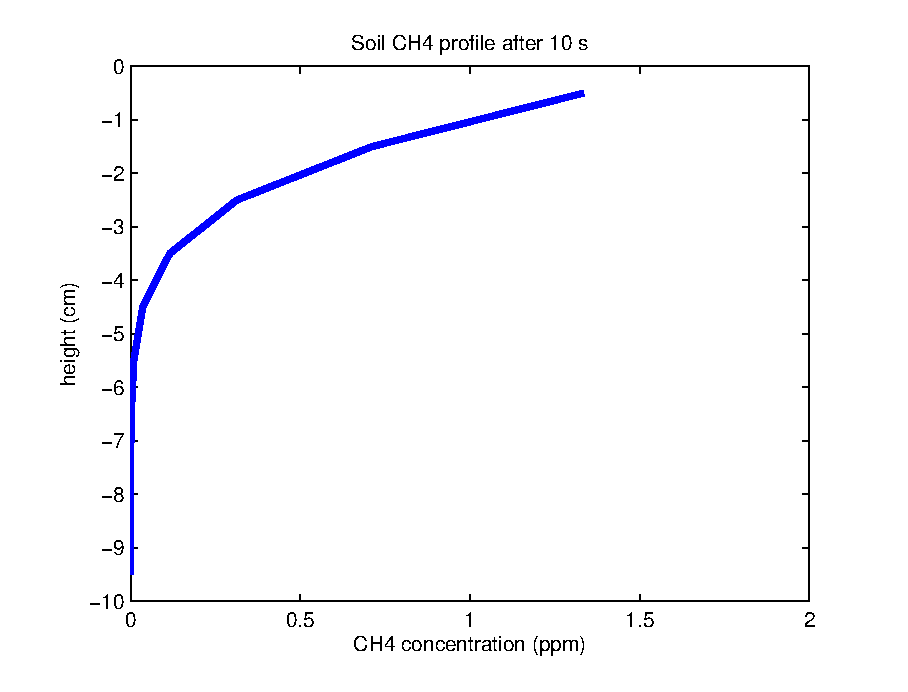
\includegraphics[width=\linewidth]{ch4-ch4model-10s.eps}
\caption{Soil profile of CH4 after 10.0s of simulation.}
\label{fig:ch4-ch4model-10s}
\end{marginfigure}

Now try a longer model run (100 s) (\texttt{>>ch4model(100.0})) and see what happens. You should get something like Figure \ref{fig:ch4-ch4model-100s}.

\begin{marginfigure}[-1.0in]
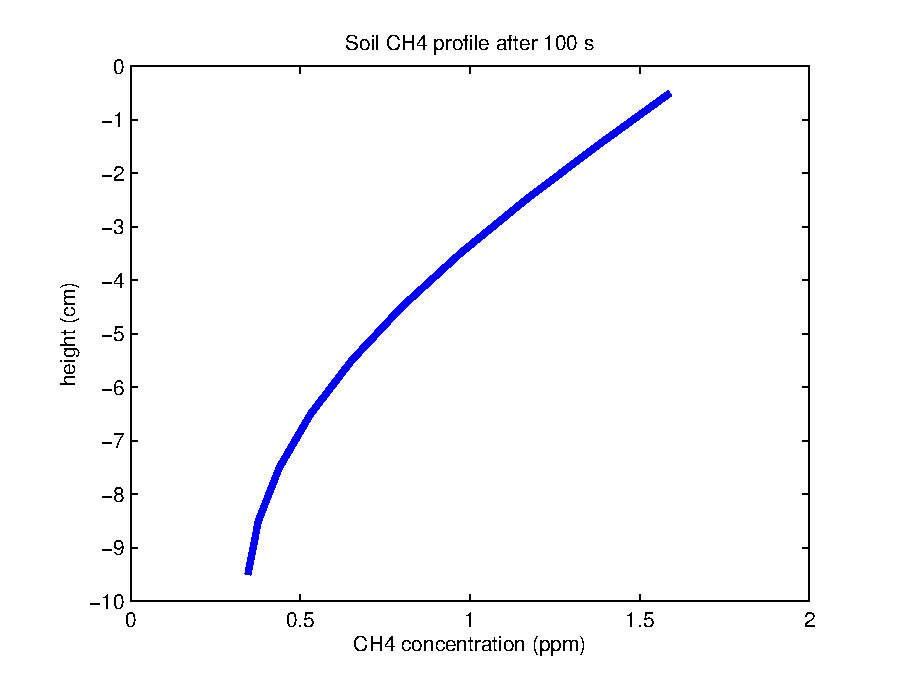
\includegraphics[width=\linewidth]{ch4-ch4model-100s.eps}
\caption{Soil profile of CH4 after 100.0s of simulation.}
\label{fig:ch4-ch4model-100s}
\end{marginfigure}

Go find out when the system (approximately) reaches equilibrium (i.e., the profile stops changing with time). You will need to judge when any further changes are so small they could not possibly really matter.

\noindent\rule[0.0ex]{\linewidth}{0.5pt}

\newthought{Keeping with the same Example}\sidenote{OVERVIEW: 
\begin{enumerate}[noitemsep]
\item adapt model and explore choice of time-step
\item adapt model and explore choice of layer thickness / number of soil layers
\item add methanotrophs (CH\(_{4}\) sinks)
\item play!
\end{enumerate}
} and having constructed the basic diffusion framework for the model, we can explore what happens if consumption of CH\(_{4}\) (by methanotrophs) occurs within the soil (as well as exploring the numerical stability and hence choice of time-step duration and grid resolution, of the model).

First, take the \texttt{ch4model} (or whatever named) function and add a second input parameter to set the time-step length. You should then have two input parameters (\texttt{maxtime} and \texttt{dt}).\sidenote{Note that you will have to comment out (or delete) the line in the code where previously you defined the time-step length as fixed with a value of 0.1 s.} By calling the function from the command line, with a model simulation duration of 100 s, play around with the time-step length. Approximately, what is the longest time-step you can take before the model becomes numerically unstable? What are the characteristics of the soil CH\(_{4}\) profile that lead you to suspect instability occurring in the numerical solution? The onset of instability might look something like Figure \ref{fig:ch4-ch4model-model2}.

\begin{marginfigure}[0.0in]
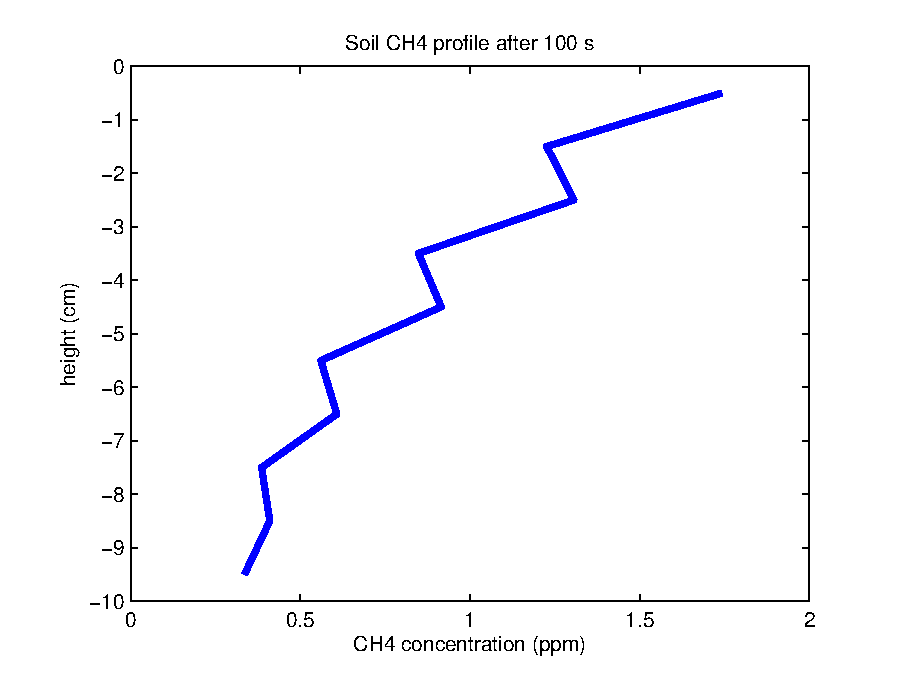
\includegraphics[width=\linewidth]{ch4-ch4model-model2.eps}
\caption{Soil profile of CH4 after 100.0s of simulation with an extremely marginal choice of time-step length.}
\label{fig:ch4-ch4model-model2}
\end{marginfigure}

Now ... it just so happens that some top profs (me!?) have told you that there are some bugs -- methanotrophs (see \textit{Ridgwell et al.} [1999]) that live  deep down in the soil. From this, you assume that they will be present only in the deepest (\(n=10\)) soil layer in the model. They just sit there, munching away on CH4 that diffuses down from the atmosphere into the soil pore-space. A bit like idle grad students living on a diet of pizzas.\sidenote{Except students mostly don't live in the cold damp dirty ground.} The bugs consume the CH4 present in the soil pore space at a rate that is proportional to the concentration of CH\(_{4}\) in the soil (makes sense -- the more CH\(_{4}\) food source there is to metabolize, the more than they will remove per second). Call this rate constant e.g. \texttt{munch\_rate}. It has units of fractional removal per second. In other words, if the concentration of CH\(_{4}\) in layer \(n=10\) is \texttt{conc(10)}, then in one second:
\begin{docspec}
munch\_rate * conc(10)
\end{docspec}
cm\(^{3}\) CH\(_{4}\) cm\(^{-1}\) will be lost from the soil pore space. So, if you had a rate constant (\texttt{munch\_rate}) of 0.5 s\(^{-1}\), then each second, half of the CH\(_{4}\) in layer \(n=10\) would be removed. Of course, the time-step in the loop might not be 1.0s -- if you had \texttt{dt=0.1}, for instance, then the loss of CH\(_{4}\) each time around the loop would be:
\begin{docspec}
0.1 * munch\_rate * conc(10)
\end{docspec}
cm\(^{3}\) CH\(_{4}\) cm\(^{-1}\). Are you following so far ... ?

Now, add a third parameter that is passed into the soil CH\(_{4}\) model function for the rate constant. Modify your equation for the updating of the CH\(_{4}\) concentration in the deepest (n=10) soil layer to reflect the presence of the methanotrophs. Call the soil CH\(_{4}\) model function; pass a time-step of 0.1 s and a methanotroph CH\(_{4}\) consumption rate constant of 1.0 s-1. Your function call should look something like this at the command line;
\begin{docspec}
>> ch4model(xxx,0.1,1.0)
\end{docspec}
where \texttt{xxx} is the duration of the simulation\sidenote{Not your favourite website address.}\sidenote[][-1.5in]{e.g. for 100s, giving a plot looking (hopefully) like Figure \ref{fig:ch4-ch4model-model3}.}. How many seconds (approximately) does it take for an equilibrium profile to be established (i.e., what was the simulation duration that you used to create your plot?). What, ultimately, is the shape of the soil profile of CH\(_{4}\) concentration, and why?

\begin{marginfigure}[-1.0in]
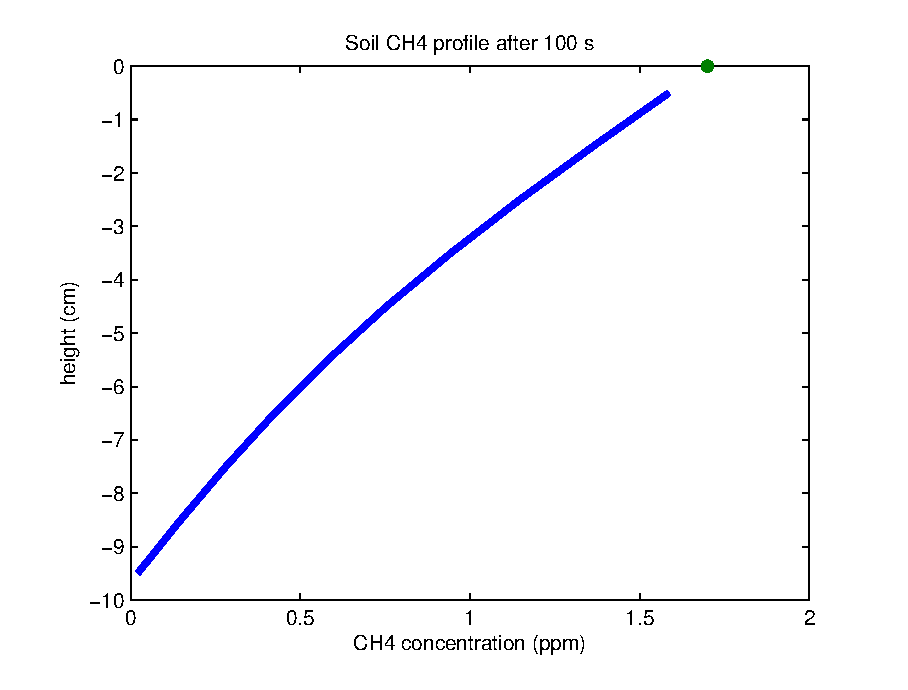
\includegraphics[width=\linewidth]{ch4-ch4model-model3.eps}
\caption{Soil profile of CH4 after 100.0s of simulation, with CH4 uptake at the base of the profile with a rate constant of 1.0 per s.}
\label{fig:ch4-ch4model-model3}
\end{marginfigure}

Now ... lets say that you then go out into the field and take samples from each 1 cm thick interval of a 10 cm soil profile. You incubate the soil samples in sealed flasks with CH\(_{4}\) initially present in the headspace (a fancy word for the air or gas above a sample in a container). Hey -- you observe that CH\(_{4}\) is removed in all flasks, equally. Someone screwed up(!) -- these bugs live throughout the soil column, not just at the bottom. You'd better update your model in light of these new scientific findings.

Add a term (within the 2nd \(n\) loop in which you update the CH\(_{4}\) concentrations) to reflect the consumption of CH\(_{4}\) in the layers \(n=1\) through \(9\). (You can keep the term for consumption in the \(n=10\) layer.) Since the bugs are spread out through 10 layers rather than being concentrated in one (at the bottom), presumably the consumption rate is only 1/10 of your previous rate value. So use munch\_rate = 0.1 (i.e., a rate constant of 0.1 s\(^{-1}\), rather than the value of 1.0 s\(^{-1}\) that you used before) for all subsequent calculations. Call the soil CH\(_{4}\) model function with a time-step length of 0.1 s and determine the steady state soil (equilibrium) CH\(_{4}\) profile (Figure \ref{fig:ch4-ch4model-model4}). What shape does this remind you of ... and why?\sidenote{There is in fact an analytical solution to this profile -- can you derive it?} 

\begin{marginfigure}[-0.0in]
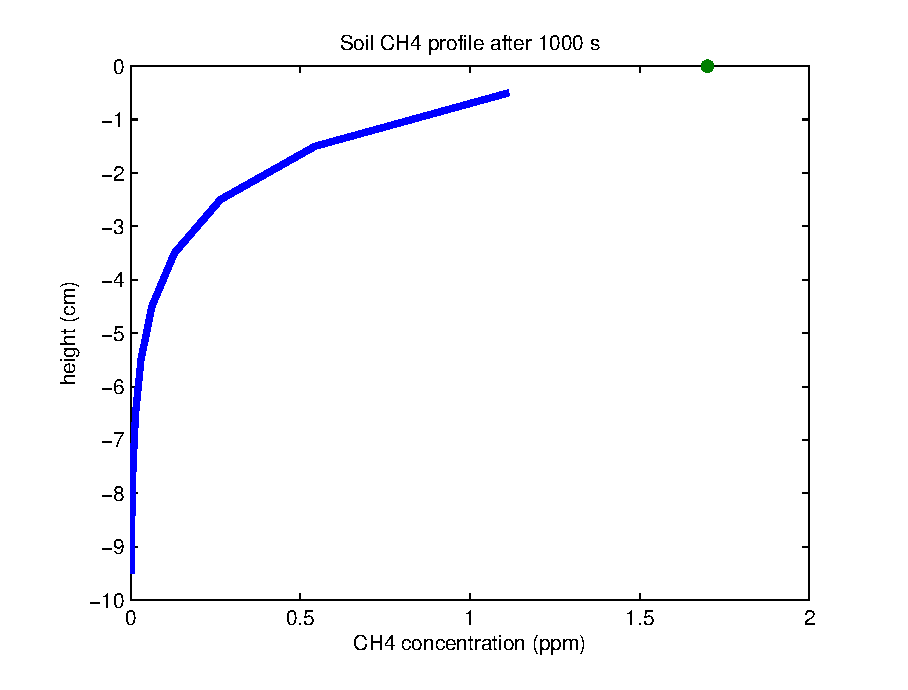
\includegraphics[width=\linewidth]{ch4-ch4model-model4.eps}
\caption{Equilibrium soil profile of CH4, with CH4 uptake throughout the soil column with a rate constant of 0.1 per s.}
\label{fig:ch4-ch4model-model4}
\end{marginfigure}

A couple of slightly more challenging modifications to try now:

\begin{enumerate}
\setlength{\itemindent}{.2in}

\item Alter the model so that you can also pass into the function, the number of soil layers that are represented in the upper 10 cm -- equivalent to altering the thickness of each layer. This change is a little more involved than simply altering the time-step duration. For instance, now, rather than \(n\) (the number of layers) going from 1 to 10, they are now counted from 1 to \(n_{max}\)\sidenote{For which you might call the variable, e.g. \texttt{n\_max}).} (the number of model layers you pass into the function)

\item Add in a parameter controlling the maximum depth of the soil column represented (replacing the fixed 10 cm assumption from previously). 

\item Try adding a source of CH\(_{4}\) at the base of the soil column.\sidenote{This is quite physically plausible and might reflect (in order of decreasing likelihood): a water-logged, anoxic layer at depth, thawing permafrost, or a natural gas seep.} \sidenote{Note that now you have 2 different boundary conditions in the model -- a fixed concentration in the atmosphere at the surface, and a fixed flux at depth.} Units should be: cm\(^{3}\) CH\(_{4}\) cm\(^{-3}\) s\(^{-1}\). But now much (i.e. what rate of methane production would be reasonable)? You could play about, trying different values until finding one that did not produce anything insane. Not a very satisfying approach. You could certainly look up in the literature measured soil production values (a much better approach). You could also get a feel for a possible order-of-magnitude by contrasting with the previous consumption flux (from the atmosphere). Actually, you have not looked at this so far (the total atmospheric CH\(_{4}\) consumption flux) and maybe should have as it is what matters in terms of the soil being an effective sink, or not, for atmospheric CH\(_{4}\). To do this -- you need to extract from the model, the CH\(_{4}\) flux from the atmosphere into the first soil layer (why?).
 Do this and make it the returned values from the function.
Now set the production (at depth) rate similar to the net (from atmosphere) consumption flux from before (with methanotrophic activity throughout the soil profile). You should obtain a profile (at steady state) that is approximately symmetrical in depth\sidenote{But not quite symmetrical -- why?} -- e.g. Figure \ref{fig:ch4-ch4model-model4}.

\begin{marginfigure}[-1.5in]
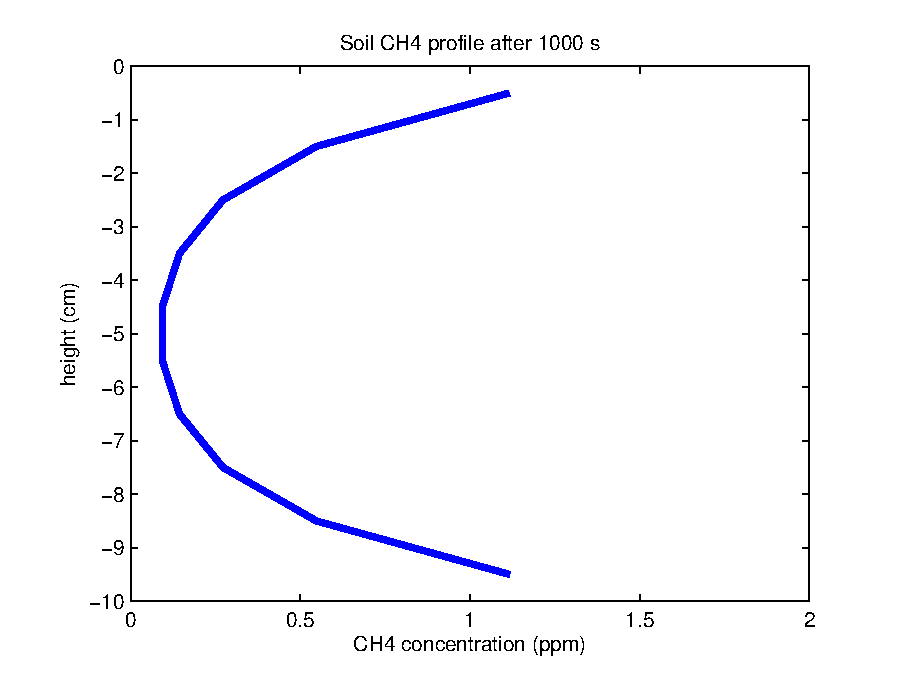
\includegraphics[width=\linewidth]{ch4-ch4model-model6.eps}
\caption{Example equilibrium soil profile of CH4 with production at depth.}
\label{fig:ch4-ch4model-model6}
\end{marginfigure}

\item Finally ... there should be (there is!) a value for the production rate at depth, at which the flux into the atmosphere is zero. (There are certainly some very large production rates at depth for which the flux from the atmosphere is negative, i.e. there are net emissions of CH\(_{4}\) *to* the atmosphere. Can you find this value (which makes the net exchange zero) ... *without* trial-and-error?\sidenote{Your function returns the net flux and you need to search for the production rate value that minimizes this net flux. Meaning you need to construct a search algorithm, testing a larger production rate of the net flux is positive, and a smaller value if the net flux it is negative.}

\end{enumerate}

%----------------------------------------------------------------------------------------
% CHAPTER 10
%----------------------------------------------------------------------------------------

\chapter{Numerical modelling meets GUIs (and prettier games!)}
\label{ch:10}

%------------------------------------------------

\newpage

%------------------------------------------------

\section{GUI Pok\'emon game}

Now we'll build on your excellent GUI skills and create a GUI interface for the ballistics (ball trajectory) model.

The idea of the 'game' is that you are going to launch a ball, the behaviour of which will be calculated as per your time-stepping ballistics model. Rather than simply detect whether or not the ball falls below zero (height), there will be a graphic (Pok\'emon) displayed and a 'hit' will be recorded if the position of the ball falls within the boundary of the graphic. The key initial conditions -- initial speed and angle of the launched ball, will be set by controls in the GUI rather than set in code. Finally, there will be a series of refinements to improve the look and feel (and game-play) of the game that will introduce a few further concepts in creating good \textbf{MATLAB} GUIs and also new \textbf{MATLAB} functions. 
Ultimately, the GUI (app) might look something like Figure \ref{fig:chGUI-pokemon1c}, but how the controls are positioned in the window and their relative size and shape, is pretty well much up to you. You could also control how the initial parameter values are set in a different way (e.g. using an \textbf{Edit Text} box rather than a \textbf{Slider}). Quite what buttons you want and how they are used is also a matter of personal aesthetics. 

\begin{marginfigure}[-5.25in]
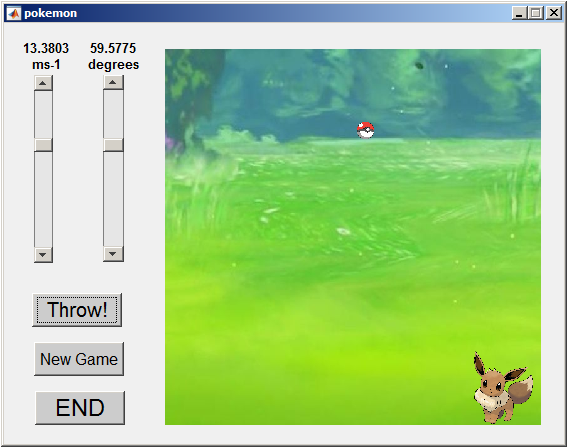
\includegraphics[width=\linewidth]{chGUI-pokemon1c.png}
\caption{Screen-shot of he Pok\'emon game App.}
\label{fig:chGUI-pokemon1c}
\end{marginfigure}

There is quite a lot of coding to be done and the risk of a huge mess ensuing. So we'll go through this all in a number of discrete steps:

\begin{description}[align=right]

\setlength{\itemindent}{-0.2in}

\item [Part \(0\)] (Some graphics tricks.)

\item [Part I] Create a basic GUI interface using \textbf{MATLAB} \texttt{guide}.

\item [Part II] Load in and display the graphics needed for the game.

\item [Part III] Add in the ballistics model.

\item [Part IV] Utilizing the sliders.

\item [Part V] Create the detection (logic) needed for a successful 'catch' and associated outcomes.

\item [Part VI] Refinements to improve the look and feel of the game.

\end{description}

\noindent Because of the complexity of the project, the complete code (\textbf{m-file}) as well as associated \texttt{.fig} GUI file, are provided (on the course webpage). These are provided if needed for guidance (e.g. what code goes where?), \uline{only}. Try your best to work through the creation of the App without this.

Example images are provided but you can substitute your own if you prefer.

If you run into unexpected and apparently nonsensical issues when you make changes and text the App, try closing the design window and any open \textsf{Figure window}s and type \texttt{>> clear all}.

\vspace{1mm}
\noindent\rule{4cm}{0.5pt}
\vspace{-2mm}

\newthought{\textit{\textbf{Part \(0\)}}} -- A few of the graphics procedures you will need to grasp and implement.

Firstly, at the command line, open a \textsf{Figure window} (\texttt{>> figure}).
Download any (legal/moral) image you care from the internet\sidenote{With the  raster graphics format being one of: \textsf{.jpg}, \textsf{.png}, \textsf{.tif}.} You can load this image into the \textbf{MATLAB} workspace with \docenvdef{imread}, and display it in the \textsf{Figure window} with \docenvdef{imshow}. (Try it.)

\marginnote{\begin{mdframed}[backgroundcolor=gray!10, roundcorner=10pt,leftmargin=1, rightmargin=1, innerleftmargin=5, innerrightmargin=5, innertopmargin=5,innerbottommargin=5, outerlinewidth=1, linecolor=light-gray]
\docenvdef{imread}
\\'\textit{\texttt{A = imread(filename)} reads the image from the file specified by \texttt{filename} ...}'
\\\noindent and in this definition, assigns the result of \texttt{imread} to a variable \texttt{A}.
\end{mdframed}}

\marginnote{\begin{mdframed}[backgroundcolor=gray!10, roundcorner=10pt,leftmargin=1, rightmargin=1, innerleftmargin=5, innerrightmargin=5, innertopmargin=5,innerbottommargin=5, outerlinewidth=1, linecolor=light-gray]
\docenvdef{imshow}
\\\texttt{imshow(A)} will  display an image held in the variable \texttt{A} (read in by \texttt{imread}).
\\\noindent Assign the result of  \texttt{imshow} to a \textit{handle} if you wish to do anything with it later, i.e.
\\\texttt{h = imshow(A);}
\end{mdframed}}

This fills up the screen, which is OK for a background image, but not for much else. Open up a new \textsf{Figure window}. You can define a set of axes anywhere in the window you like via the \texttt{axes} function:
\begin{docspec}
axes('pos',[x,y,dx,dy])
\end{docspec}
where (\texttt{x},y) are the co-ordinates in the window, which by default are from \(0-1\) in both \textit{x} and \textit{y} directions. \texttt{dx} and \texttt{dy} are the width and height, respectively, of the axes (in the same window coordinate system).

For instance, to create a set of axes starting at the origin, but only 25\% of the full width and height of the window:
\begin{docspecbold}
>> axes('pos',[0.0,0.0,0.25,0.25]);
\end{docspecbold}
If you now display the image:
\begin{docspecbold}
>> imshow(A);
\end{docspecbold}
\sidenote{Or whatever you called the variable with the image in.} you should see a smaller version of the image, positioned at the origin. If you remembered to assign the handle to a variable:
\begin{docspecbold}
>> h = imshow(A);
\end{docspecbold}
you can then delete the image:
\begin{docspecbold}
>> delete(h);
\end{docspecbold}

\noindent OK -- now dig up the \textit{script} for your ball-throwing animation -- the one where the \texttt{scatter} plotting ball location \textit{object} was deleted after a pause (giving the impression of movement/animation)\sidenote{From Part IV of Section 8.1}. Near the start of the \textit{script} (before the loop starts), load in the Pok\'eball graphic\sidenote{(or pick your own graphic)}. Then, instead of using the \texttt{scatter} function to plot a single point (circle), you are going to:
\begin{enumerate}[noitemsep]
\setlength{\itemindent}{.2in}

\vspace{1mm}
\item Define an \texttt{axes} object, either centered (harder)  on the position of the ball that \texttt{scatter} plotted, or taking as its origin (easier), the position of the ball. The width and height of the axis ... you can play about with, but it should be a relatively small proportion of the total size of the main axes.
\\Note ... that axes uses relative coordinates (i.e. \(0-1\) in both dimensions) and not your actual ball position (in units of \(m\)). So you'll need to determine the horizontal and vertical position of the ball, \uline{as a fraction}, of the total size of your domain.\sidenote{e.g. you might have considered a maximum horizontal distance of \(10m\) and a maximum vertical distance of \(7.5m\) and specified:
\begin{docspecmargin}
axis([0 10 0 7.5]);
\end{docspecmargin}
In which case, for the position of the ball in relative/normalized units -- divide the \textit{x} position by \(10\) and the \textit{y} position by \(7.5\).
\\So, if your \(x\) and \(y\) positions were given by \texttt{h(1)} and \texttt{h(2)}, respectively, the corresponding coordinates of the frame are then: \\\texttt{h(1)/10}, \texttt{h(2)/7.5}.}
\\It is important here not to be confused between the different sets of axes -- you defined the primary one, outside of the loop, and which  defines the domain in which the trajectory is simulated:
\begin{docspec}
axes(\textcolor[rgb]{1,0,1}{'Position'},[0 0 1 1],\textcolor[rgb]{1,0,1}{'Visible'},\textcolor[rgb]{1,0,1}{'off'});
\end{docspec}
you then specified what (\textit{x,y}) limits the axes represented, e.g.:
\begin{docspec}
axis([0 x\_max 0 y\_max]);
\end{docspec}
(here, use parameters containing the maximum \textit{x} and \textit{y} limits). You then \texttt{scatter} plot the ball's position in the \(x_{max}\),\(y_{max}\) domain.
\\In contrast ...  to contain (display) the image you are defining a small axes region (within the loop). The location and width/height of this graphics frame are given in relative (\(0-1\) scale) units, rather than \(0-x_{max}\) and \(0-y_{max}\) you assumed with \texttt{scatter}.
\\The line:
\begin{docspec}
axes('pos',[x,y,dx,dy])
\end{docspec}
(where you need to replace \texttt{[x,y,dx,dy]} with the appropriate coordinates and image size - see margin note for an example of deriving the correct coordinates) comes in the code in place of scatter.  

\vspace{1mm}
\item Plot the ball image (i.e. add the command \texttt{imshow}, which should come immediately after the \texttt{axes} command). Assign the graphics \textit{handle} returned by the function to a variable.

\vspace{1mm}
\item As per previously, after a delay, you can delete the graphic object,

\end{enumerate}

Omitting \texttt{delete(h)}, the output of your ball/trajectory model should look like Figure \ref{fig:ch10-pokeball1}.

\begin{marginfigure}[0.0in]
\includegraphics[width=\linewidth]{ch10-pokeball1.eps}
\caption{Trajectory model, with a Pok\'eball image replacing the \texttt{scatter} point. Here show without deleting the image once displayed.}
\label{fig:ch10-pokeball1}
\end{marginfigure}

\vspace{1mm}
\noindent\rule{4cm}{0.5pt}
\vspace{-2mm}

\newthought{\textbf{\textcolor{red}{OPTIONAL}}} -- Ignoring the fact that image deleting is disabled, the images (\textit{sprites}) Figure \ref{fig:ch10-pokeball1} have a black background around them. Yuk. If you picked an image with a white background, it would look better, unless you had a dark background to the entire figure window.\sidenote{You could pick an image which is square. But what balls have you seen that are cubes? Seriously. Do you get out at all an play any sports? Or even watch TV?!??}

Some (raster) graphics formats enable a 'transparency' to be defined -- basically a color that ... is transparent. Common formats with such a capability include \textsf{.gif} and \textsf{.png}. As \textsf{.png} is a valid format for \texttt{imread} -- try and find a \textsf{.png} image on the internet with a transparency.\sidenote{In Google search / images, a transparent background is illustrated as a grey-white checkerboard.} You could also use the Pok\'eball image provided (which has a transparent background).

To enact a transparent background in \textbf{MATLAB} is a bit of a mess ... you first have to obtain additional handles when you read in the image:
\begin{docspec}
[img\_ball, h\_map\_ball, h\_alpha\_ball] = imread(\textcolor[rgb]{1,0,1}{'Pokeball.png'});
\end{docspec}
where \texttt{img}\_ball is the variable containing the ball image, as before, and \texttt{h\_alpha\_ball} is a handle to ... lets not worry about what it is to. Just that you need it.

When you plot the ball, now add an additional command:
\begin{docspec}
    h = imshow(img\_ball);
    set(h, \texttt{'AlphaData'}, h\_alpha\_ball);
\end{docspec}
which sets this thing I am not telling you about.\sidenote{Wikipedia (please donate!), says: '\textit{In computer graphics, alpha compositing is the process of combining an image with a background to create the appearance of partial or full transparency.}' Without alpha channel information, everything is assumed 100\% opaque (including the background).}

For instance -- the same model as before (with the Pok\'eball replacing \texttt{scatter} but with the use of \texttt{delete}), but with only \(1s\) simulated, plus a background image displayed (before the loops starts), and ... with a transparency implemented (removing the square black background), looks like Figure \ref{fig:ch10-pokeball2}.

\begin{marginfigure}[0.0in]
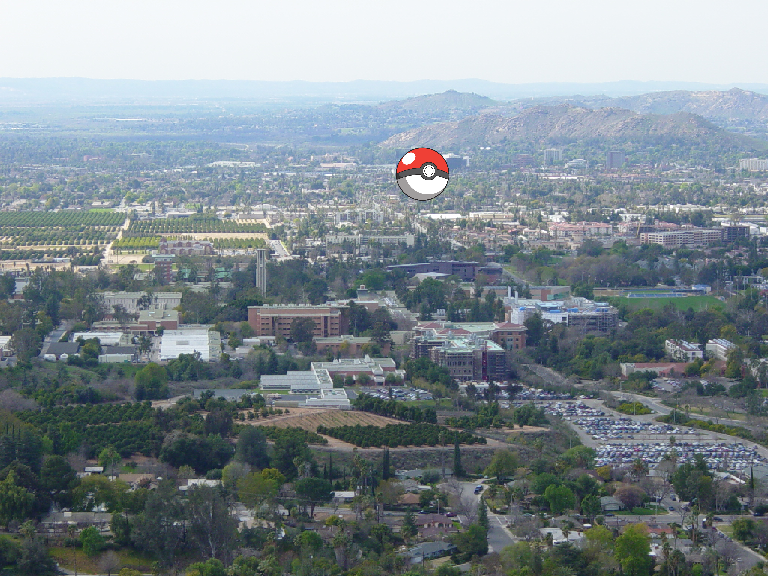
\includegraphics[width=\linewidth]{ch10-pokeball2.png}
\caption{Trajectory model (exactly the same trajectory as per the Figure \ref{fig:ch10-pokeball1}), frozen mid-flight at \(t=1s\) with the Pok\'eball passing over UC-Riverside.}
\label{fig:ch10-pokeball2}
\end{marginfigure}

Now ... we are ready ...

\vspace{1mm}
\noindent\rule{4cm}{0.5pt}
\vspace{-2mm}

\newthought{\textit{\textbf{Part I}}} -- the basic GUI.

To achieve a GUI along the lines of Figure \ref{fig:chGUI-pokemon1c} you need to create the following objects in the window design editor (but don't create them quite yet -- details will follow ...):

\begin{enumerate}[noitemsep]
\setlength{\itemindent}{.2in}
\item Something to display all the action and graphics in. This is pretty well much like \textbf{MATLAB} creates when you use \texttt{plot}, \texttt{scatter}, or any of the graphical functions that create a \textsf{Figure Window}. This is called an \textsf{Axes} object. 
\item A \textbf{Push Button} for telling \textbf{MATLAB} to start calculating (and displaying) the balls' trajectory.
\item A \textsf{Push Button} for resetting the game once it is finished.\sidenote{This we'll only worry about making use of this in Part IV.}
\item A \textsf{Push Button} to finish the game and close the App.
\item A \textsf{Slider} (bar) to set the initial speed of the ball.
\item A \textsf{Slider} to set the initial angle of the balls' trajectory.
\item For each slider bar: a \textsf{Static text box} to display the value.
\item Also for each slider bar: a \textsf{Static text box} to display the units.
\end{enumerate}

Make a start by running \textbf{GUIDE} at the command line. Create a new (blank) GUI. You might save it once the GUI editor window has open up\sidenote{\textbf{\uline{F}ile} -- \textbf{Save \uline{A}s\ldots}}. \textbf{MATLAB} then opens the \textsf{Editor} and the GUI code template.

Sketch out on a piece of paper how you might lay out the objects in your GUI window before you actually start to create anything.
If you have graph paper to hand, you could sketch out your design on a grid similar to the design window grid and size. Note that should should be aiming to make the \textsf{Axes} object square (i.e. the same length in both \textit{x} and \textit{y} dimension) as the background image we are going to use is square.\sidenote{Later on you might want to try substituting your own background image. In this situation, you might need a different aspect ratio to the \textbf{Axes} object.} Also note that the \textsf{Sliders} can be horizontal rather than vertical if you prefer and if it make it easier to pack in all the objects.

OK -- to begin for real.

\begin{enumerate}
\setlength{\itemindent}{.2in}

\item You have to start somewhere (i.e. you have to pick on one object as the first one to be created!), and the best place to start is arguably with the \textsf{Axes} object as it is the largest object in your window. Click on the \textsf{Axes} icon and drag out the position and size of the object you want.\sidenote{Note that you can drag the GUI editor window larger, and you can also drag larger the gridded design area, meaning that your App window will be larger that you run the program.} By default, it is assigned a name (its \textsf{Tag} property) of \textsf{axes1}. You are not going to have so desperately many objects that it is necessarily worth re-naming it, but you can if you wish (although the text will refer to \textsf{axes1} where needed). Remember that you can move and re-size it at any point after creating it. Its position as \textit{x},\textit{y} of the objects origin as well as dimensions (\textit{x}-length and \textit{y}-height) are indicated by \textsf{Position} at the bottom right of the design window. For e.g. creating an approximately square \textsf{Axes} object, you can also simply count the number of grid lines in each dimension.

Save the \textsf{.fig} file and run it\sidenote{Note that there are two things that potentially might both need being saved -- the \textbf{m-file} and the \textbf{.fig} file. If you make code changes, save the \textbf{m-file}, and if you make design change sin the GUI editor, save the \textbf{.fig} file.}. You do indeed have a graph-like object with labelled axes. This is not actually that convenient (to have the axes labels when you don't need any in this particular example). In the design window -- double
click on the \textsf{Axes} object to bring up its list of properties. Find and edit \textsf{XTick} -- delete all the tick mark numbers. Do the same for the y-axis. Close the GUI window from the previous version if it is still open, then save and re-run. Now you should see a large white square(ish) with two thin black lines delineating the axes\sidenote{We could remove these black lines, but they'll get covered up later.}, and nothing else.

\item Next \textit{Push Button} \#1. Create (position and size, where- and how-ever you think best). Simplest is to leave the default name ('\textsf{pushbutton}1'). Change the text associated with the \textit{Push Button} (property '\textsf{String}'). Label as 'Throw', 'Go', or whatever seems appropriate. Remember that you can change the default font size, family, color ... (and e.g. make bold etc.) as well as the color of the button itself (plus a host of other property options).

\item Create a 2nd \textit{Push Button} ('\textsf{pushbutton}2') as per before. Label consistent with the GUI\ aim (and e.g. Figure \ref{fig:chGUI-pokemon1c} ).

\item Similarly, create 3rd \textit{Push Button} ('\textsf{pushbutton}3').

\item Now we need a \textsf{Slider}\sidenote{Not anything to do with baseball.} bar. These are bar with a slider ('knob') that can be slide up and down via the mouse, or moved by clicking in the bar above or below the position of the slider. By doing so (changing the position of the slider along the slider bar), you change the numerical value of the slider. We are going to use one in order to set the initial speed of the ball. So go create one (leaving the default name of '\textsf{slider1}').

Because we need to link the \textsf{Slider} to our model (in terms of parameter value), we need to specify a minimum and maximum value that the \textsf{Slider} can take, as well as an initial value. These properties can be set at in the code, but we'll start off by specifying them using the design GUI tool. If you double click on the \textsf{Slider} you'll get its property list opened up. The minimum and maximum property value name are \textsf{Min} and \textsf{Max} -- edit these to span a plausible initial speed range\sidenote{I used \(0\) to \(20 ms^{-1}\).}. Also set a default initial value (parameter name '\textsf{Value}')\sidenote{I assumed \(0 ms^{-1}\).}.

\item Create a second \textsf{Slider} ('\textsf{slider2}') for setting the initial angle of the ball (\textit{theta}).\sidenote{Here I assumed a range of \(0\) to \(90 \degree \), with a default of \(0 \degree \).}

\item Because the \textsf{Sliders} themselves do not tell you quite what value you have slide the slider to, it is a Good Idea to somewhere display the value. We'll do this via a \textsf{Static Text} box ('\textsf{text1}') and you'll need to create one to go with each \textsf{Slider} (so you'll also have a '\textsf{text2}' named object). For now -- simply leave the default text as is.

\item Finally, if you follow the design in Figure \ref{fig:chGUI-pokemon1c}, you could add a further pair of \textsf{Static Text} boxes in order to display the units. This is far from essential and I'll leave it up to you whether you bother, particularly if your window is cluttered already. 

\end{enumerate}

That is the basic GUI design done. Save and run (having first closed any open, running, instances of your GUI program). You should have a window with all the objects discussed, but with none of them yet doing anything.

At this point it is worth quickly orientating you around the automatically-generated code \textsf{m-file}:

\vspace{-2mm}
\begin{itemize}[noitemsep]
\setlength{\itemindent}{.3in}
\vspace{1mm}
\item At the very top of the \textbf{m-file} appears:
\begin{docspec}
\textcolor{blue}{function} varargout = Pokemon(varargin)
\end{docspec}
which defines the main program function (here,  called \texttt{pokemon} and meaning the App is run by typing \texttt{>> Pokemon}). \\\uline{Remember that you do not have to edit any of this function.}
\vspace{1mm}
\item Next comes:
\begin{docspec}
\textcolor[rgb]{0,0.501961,0}{\% --- Executes just before Pok\'emon is made visible.}
\\\textcolor{blue}{function} Pokemon\_OpeningFcn(hObject, eventdata, handles, varargin)
\end{docspec}
This is the function that is called just before the window is made visible and we'll edit it later in order to carry out some initial tasks (i.e. before the ballistics model itself runs).
\vspace{1mm}
\item Then:
\begin{docspec}
\textcolor[rgb]{0,0.501961,0}{\% --- Outputs from this function are returned to the command line.}
\\\textcolor{blue}{function} varargout = Pokemon\_OutputFcn(hObject, eventdata, handles)
\end{docspec} 
which is mysteriously useless and \uline{we will not edit}.
\vspace{1mm}
\item The first actually useful automatically generated code is:
\begin{docspec}
\textcolor[rgb]{0,0.501961,0}{\% --- Executes on button press in pushbutton1.}
\\\textcolor{blue}{function} pushbutton1\_Callback(hObject, eventdata, handles)
\end{docspec} 
This will contain the code that is executed when the 'Throw' (or 'Go') button ('\textsf{bushbutton1}') is pressed and will end up containing the complete ballistics model code.
\vspace{1mm}
\item The function code for when second button ('\textsf{bushbutton2}') is pressed appears in order after the function associated with '\textsf{bushbutton1}':
\begin{docspec}
\textcolor[rgb]{0,0.501961,0}{\% --- Executes on button press in pushbutton2.}
\\\textcolor{blue}{function} pushbutton2\_Callback(hObject, eventdata, handles)
\end{docspec} 
We'll only make use of this towards the very end of this section is making the final refinements to the App.
\vspace{1mm}
\item Then, the third button ('\textsf{bushbutton3}'):
\begin{docspec}
\textcolor[rgb]{0,0.501961,0}{\% --- Executes on button press in pushbutton3.}
\\\textcolor{blue}{function} pushbutton3\_Callback(hObject, eventdata, handles)
\end{docspec} 
This will contain more more than a command to close the App (as you have programmed previously).
\vspace{1mm}
\item The code that is called whenever the position of the first slider the appears:
\begin{docspec}
\textcolor[rgb]{0,0.501961,0}{\% --- Executes on slider movement.}
\\\textcolor{blue}{function} slider1\_Callback(hObject, eventdata, handles)
\end{docspec} 
\vspace{1mm}
\item This is then followed by a second function associated with \textsf{slider1} whose purpose is ... not obvious. Perhaps slider initialization? Regardless, we'll be ignoring the following code:
\begin{docspec}
\textcolor[rgb]{0,0.501961,0}{\% --- Executes during object creation, after setting all properties.}
\\\textcolor{blue}{function} slider1\_CreateFcn(hObject, eventdata, handles)
\end{docspec} 
\vspace{1mm}
\item The final code is the pair of functions for the 2nd slider (of which we'll only edit the first of these two functions (\texttt{slider2\_Callback})):
\begin{docspec}
\textcolor[rgb]{0,0.501961,0}{\% --- Executes on slider movement.}
\\\textcolor{blue}{function} slider2\_Callback(hObject, eventdata, handles)
\end{docspec} 
\begin{docspec}
\textcolor[rgb]{0,0.501961,0}{\% --- Executes during object creation, after setting all properties.}
\\\textcolor{blue}{function} slider2\_CreateFcn(hObject, eventdata, handles)
\end{docspec} 
\end{itemize}

Before we move on, you could add your first code to the \textsf{m-file} -- a close action if you click on the lower of the three \textsf{Push Buttons}. Refer to the previous sub-section and example to remind yourself how to do this. You are aiming to have the App window close when you click on \textsf{pushbutton3}, whose associated function is called \texttt{\textcolor{blue}{function} pushbutton3\_Callback}.

Save the \textsf{m-file} and re-run the App by typing its name (e.g. \texttt{>> Pokemon}) and the command line (first closing any already open instances of it). The App window should now close when you click on the third button. In the GUI design editor, edit the 'value' of the \textsf{String} property of this \textsf{Push Button} so that it has a logical and vaguely meaningful label. 

\vspace{1mm}
\noindent\rule{4cm}{0.5pt}
\vspace{-2mm}

\newthought{\textit{\textbf{Part II}}} -- (graphics) initialization. 

\noindent Note that in this section, \uline{all} the code will go in \texttt{\textcolor{blue}{function} Pokemon\_OpeningFcn}, \uline{after} the following (automatically generated) lines:
\begin{docspec}
\textcolor[rgb]{0,0.501961,0}{\% Choose default command line output for Pok\'emon}
\\handles.output = hObject;
\textcolor[rgb]{0,0.501961,0}{\\\% Update handles structure}
\\guidata(hObject, handles);
\textcolor[rgb]{0,0.501961,0}{\\\% UIWAIT makes Pok\'emon wait for user response (see UIRESUME)
\\\% uiwait(handles.figure1);}
\end{docspec}

\noindent First, we'll read in a background image ('background.jpg' -- available for download from the  website, \uline{or pick your own}) and then display it. We'll use the commands \texttt{imread} for reading in the graphics format (and converting it into something \textbf{MATLAB} prefers) and then \texttt{imshow} to display it. The first part is easy enough:
\begin{docspec}
img\_background = imread(\textcolor[rgb]{0.501961,0,1}{'background.jpg'});
\end{docspec}
The question then becomes 'where' to display it. You might not think there is even a question in this -- in the window! Except ... where in the window?

We actually want the background image in the (currently) blank \textsf{Axes} area, not just anywhere in the \textsf{Figure window} (which also have various button etc. objects positioned in it). We need to find the ID of the \textsf{Axes} object and tell \textbf{MATLAB} that is 'where' we want to display it.\sidenote{Actually, it may work without worrying about this, but we'll need to be able to specify where to position other images later anyway.} We can get the \textit{handle} (ID) of the \textsf{Axes} object via:
\begin{docspec}
h\_axes = findobj(\textcolor[rgb]{0.501961,0,1}{'Tag'},\textcolor[rgb]{0.501961,0,1}{'axes1'});
\end{docspec}
and then tell \textbf{MATLAB} that this is currently the object to put things in by:
\begin{docspec}
axes(h\_axes);
\end{docspec}
(which sets the current/active axes object to the one with the handle \texttt{h\_axes})).
We then use this handle in the call to \texttt{imread}:
\begin{docspec}
h\_background = imshow(img\_background,\textcolor[rgb]{0.501961,0,1}{'Parent'},h\_axes);
\end{docspec}
Try it (run the App). (The only problem with this is that \textbf{MATLAB} may completely fail to scale the image to fit the \textsf{Axes}. We'll fix this shortly.)

While we're at it (editing \texttt{\textcolor{blue}{function} Pokemon\_OpeningFcn}), we can specify the axis range for plotting the position of the ball in the Axes object (as you did previously), and add a \texttt{hold on} for completeness. We may as well then also define the axis ranges (in \(m\)) as parameters (that we can use elsewhere).

The complete code (so far), at the end of the automatically generated code in \texttt{\textcolor{blue}{function} Pokemon\_OpeningFcn}, becomes:
\begin{docspec}
\textcolor[rgb]{0,0.501961,0}{\% define grid dimensions}
\\x\_max = 10.0;
\\y\_max = 10.0;
\\\textcolor[rgb]{0,0.501961,0}{\% read in background image}
\\img\_background = imread(\textcolor[rgb]{0.501961,0,1}{'background.jpg'});
\\\textcolor[rgb]{0,0.501961,0}{\% set axes suitable for game}
\\axes(h\_axes);
\\axis([0 x\_max 0 y\_max]);
\\hold \textcolor[rgb]{0.501961,0,1}{on};
\\\textcolor[rgb]{0,0.501961,0}{\% draw background}
\\h\_background = imshow(img\_background,\textcolor[rgb]{0.501961,0,1}{'Parent'},h\_axes, ...
\\'Xdata',[0 x\_max],'Ydata',[0 y\_max]);
\end{docspec}
Here -- as part of the call to \texttt{imshow}, the size and position of the image are now explicitly prescribed (and the image scaled to completely fill the \textsf{axes} object).

When you run all this, you should get Figure \ref{fig:chGUI-pokemon2} (or with alternative background). 

\begin{marginfigure}[0.0in]
\includegraphics[width=\linewidth]{chGUI-pokemon2.png}
\caption{Template App with background image.}
\label{fig:chGUI-pokemon2}
\end{marginfigure}

Next, we want a Pok\'emon to throw the ball at! The load-in code (which can go \uline{after} the code fragment above) for the image is identical to before:
\begin{docspec}
img\_eevee = imread(\textcolor[rgb]{0.501961,0,1}{'Eevee.png'});
\end{docspec}
(the image itself ('\textsf{Eevee.png}') can be replaced with your own ...) 

There are two complications in using \texttt{imread}, however. To see what these complications are, after the \texttt{img\_eevee = } line, add the following:
\begin{docspec}
h\_eevee = imshow(img\_eevee,\textcolor[rgb]{0.501961,0,1}{'Parent'},h\_axes);
\end{docspec}
to also display the image. Well, it is a bit of an odd mess. By default, \texttt{imshow} tries to fit an image to the space, so that might, at least partly, help explain things.

We can start by making the Pok\'emon image smaller and see whether that helps us to work out what is going on. To do this, we could e.g. pick half of the size of the \textsf{Axes} object, and plot the Pok\'emon from the origin. A replacement line to do this would look like: 
\begin{docspec}
h\_eevee = imshow(img\_eevee,\textcolor[rgb]{0.501961,0,1}{'Parent'},h\_axes,\textcolor[rgb]{0.501961,0,1}{'Xdata'},[0 x\_max/2],\ldots
\\\textcolor[rgb]{0.501961,0,1}{'Ydata'},[0 y\_max/2]);
\end{docspec}
When you run this, you should get Figure \ref{fig:chGUI-pokemon3}. 

\begin{marginfigure}[0.0in]
\includegraphics[width=\linewidth]{chGUI-pokemon3.png}
\caption{Template App with background image plus Pok\'emon.}
\label{fig:chGUI-pokemon3}
\end{marginfigure}

You can see firstly that the Pok\'emon image is  half the size of the space -- exactly as we requested via \texttt{\textcolor[rgb]{0.501961,0,1}{'Xdata'},[0 x\_max/2]} which says to start the image at zero on the \textit{x}-axis and stretch it horizontally until half way along (\texttt{x\_max/2}), and similarly for the \textit{y}-axis. Except ... in the \textsf{Axes} object, it seems that the \textit{y}-axis origin starts at the \uline{top} and is positive downwards (which is why the Pok\'emon appears in the top left, rather than bottom left, corner).

To cut a long story short, we can generalize the position and size of the Pok\'emon that is displayed (and use this at the end when we refine the App), via the following  code fragment\sidenote{You should delete the lines starting \texttt{img\_eevee = } and \texttt{h\_eevee = } first. This 10-line code fragment then follows directly on from the previous 11-line one.}:
\begin{docspec}
\textcolor[rgb]{0,0.501961,0}{\% define Pokemon size}
\\dx\_Pokemon = 0.2*x\_max;
\\dy\_Pokemon = 0.2*y\_max;
\\\textcolor[rgb]{0,0.501961,0}{\% define initial Pok\'emon position}
\\x\_Pokemon = x\_max-dx\_Pokemon;
\\y\_Pokemon = y\_max-dy\_Pokemon;
\\\textcolor[rgb]{0,0.501961,0}{\% read in Pokemon image}
\\img\_eevee = imread(\textcolor[rgb]{0.501961,0,1}{'Eevee.png'});
\\\textcolor[rgb]{0,0.501961,0}{\% draw Pok\'emon}
\\h\_eevee = imshow(img\_eevee,\textcolor[rgb]{0.501961,0,1}{'Parent'},h\_axes,\textcolor[rgb]{0.501961,0,1}{'Xdata'},[x\_Pokemon\ldots
\\ x\_Pokemon+dx\_Pokemon],\textcolor[rgb]{0.501961,0,1}{'Ydata'},[y\_Pokemon-dy\_Pokemon y\_Pokemon]);
\end{docspec}
Now giving you a small Pok\'emon -- in fact, 20\% of the \textsf{Axes} size as specified by the parameters: \texttt{dx\_Pok\'emon} and \texttt{dy\_Pokemon}.
\\\noindent\uline{Remember that you can refer to the complete code to see how things fit together.}

If you run this, you should get Figure \ref{fig:chGUI-Pokemon4}. (Note that because \textit{y} is measured downwards from the top in the GUI \textsf{Axes} object, for \textcolor[rgb]{0.501961,0,1}{\texttt{'Ydata'}}, we write  the \textit{y} min and max values the other way around: \texttt{[y\_Pokemon-dy\_Pokemon y\_Pokemon]}.)
\begin{marginfigure}[0.0in]
\includegraphics[width=\linewidth]{chGUI-Pokemon4.png}
\caption{Template App with background image plus small Pok\'emon at bottom right.}
\label{fig:chGUI-Pokemon4}
\end{marginfigure}

One final thing  is the background to the Pok\'emon image. The original format (png) is actually defined with a transparent background. \textbf{MATLAB} can make use of this with a small tweak to the code -- replacing the \texttt{img\_eevee = } line with:
\begin{docspec}
[img\_eevee,h\_map\_eevee,h\_alpha\_eevee] = imread('Eevee.png');
\end{docspec}
which grabs additional graphics information and specifically about the transparency. And after the last line (\texttt{h\_eevee = }), add:
\begin{docspec}
set(h\_eevee,'AlphaData',h\_alpha\_eevee);
\end{docspec}
which implements the transparent background and hopefully gives you Figure \ref{fig:chGUI-Pokemon5}.

\begin{marginfigure}[0.0in]
\includegraphics[width=\linewidth]{chGUI-Pokemon5.png}
\caption{Template App with background image plus small Pok\'emon at bottom right, now with its transparency applied.}
\label{fig:chGUI-Pokemon5}
\end{marginfigure}

\vspace{1mm}
\noindent\rule{4cm}{0.5pt}
\vspace{-2mm}

\newthought{\textit{\textbf{Part III}}} -- incorporating the ballistics model.

\noindent Here -- almost all the code in this section will go into \texttt{\textcolor{blue}{function} \\\noindent pushbutton1\_Callback} -- the function that is executed when the first \textsf{Push Button} is clicked. But before any coding -- ensure that the text label associated with the first \texttt{Push Button} is appropriate for launching the ball ('Throw', 'Go!', whatever).\sidenote{Remember -- double-click on the \textsf{pushbutton1} object in the design editor and then find and edit the value of the \textbf{String} property.}

Below is a simple rendition of the ballistics model. All that has been modified from a stand-alone \textsf{m-file} that would plot the trajectory of a ball, is that the creation of a figure (and associated \texttt{hold on}) is not necessary (because this has already been done within the initialization function). Either copy-paste your own version (and comment out the figure creation line), or add the below version.

\begin{docspecmargin}
\% model constants
\\g = 9.81;
\\\textcolor[rgb]{0,0.501961,0}{\% model parameters}
\\theta0 = 80.0;
\\s0 = 5.0;
\\h0 = 2.0;
\\\textcolor[rgb]{0,0.501961,0}{\% model parameters -- time (s)}
\\dt = 0.05;
\\t\_max = 10.0;
\\\textcolor[rgb]{0,0.501961,0}{\% calculate initial velocity components}
\\u = s0*cos(pi*theta0/180.0);
\\v = s0*sin(pi*theta0/180.0);
\\\textcolor[rgb]{0,0.501961,0}{\% set initial position of ball}
\\x = 0.0;
\\y = h0;
\textcolor[rgb]{0,0.501961,0}{\\\% create Figure window and hold on
\\\%Figure;
\\\%hold on;}
\\\textcolor[rgb]{0,0.501961,0}{\% run model}
\\\textcolor{blue}{for} t=dt:dt:t\_max,
\\ \ \ \ \    \textcolor[rgb]{0,0.501961,0}{\% update horizontal and vertical positions}
\\ \ \ \ \    dx = dt*u;
\\ \ \ \ \    x = x + dx;
\\ \ \ \ \    dy = dt*v;
\\ \ \ \ \    y = y + dy;
\\ \ \ \ \    \textcolor[rgb]{0,0.501961,0}{\% plot current position of ball}
\\ \ \ \ \    scatter(x,y);
\\ \ \ \ \    \textcolor{blue}{if} (y < 0.0)
\\ \ \ \ \ \ \ \ \        \textcolor{blue}{break};
\\ \ \ \ \    \textcolor{blue}{end}
\\ \ \ \ \    \textcolor[rgb]{0,0.501961,0}{\% update vertical velocity (horizontal velocity unchanged)}
\\ \ \ \ \   dv = -dt*g;
\\ \ \ \ \   v = v + dv;
\\\textcolor{blue}{end}
\end{docspecmargin}

When you run the complete App, and press the first \textsf{Push Button}, you should see the balls' trajectory plotted. Upside-down! WTF!?

Well, this does seem to be the coordinate system in this \textsf{Axes} object. We can fix this by subtracting the model calculated height (\texttt{y}) from the maximum y-axis value (\texttt{y\_max}) and adjust the \texttt{scatter} code line to:
\begin{docspec}
\ \ \ \    scatter(x,y\_max-y);
\end{docspec}
Except ... we defined \texttt{y\_max} in the initialization function, and its value is not available in this function, unless we define it as \texttt{global} in both, so lets do that -- add the following lines:
\begin{docspec}
global x\_max;
\\global y\_max;
\end{docspec}
to both the following functions
\begin{itemize}[noitemsep]
\setlength{\itemindent}{.2in}
\item \texttt{\textcolor{blue}{function} Pokemon\_OpeningFcn}
\item \texttt{\textcolor{blue}{function} pushbutton1\_Callback }
\end{itemize}
(before any of your other code in these files, but below anything that \textbf{MATLAB} generated automatically in the first place).

It works(!) and in the right direction (for 'up'), but it is hardly \textbf{iTunes} grade App material. What we can do, is to replace the point plotted by \texttt{scatter}, with an image.

At the top of \texttt{\textcolor{blue}{function} pushbutton1\_Callback} (after the \texttt{global} declarations) load in a ball image:
\begin{docspec}
[img\_ball, h\_map\_ball, h\_alpha\_ball] = imread('Pokeball.png');
\end{docspec}
(using the full format of returned parameters because we'll make use of its transparency). We'll then define the size of the ball:
\begin{docspec}
dx\_ball = 0.05*x\_max;
\\dy\_ball = 0.05*y\_max;
\end{docspec}
and finally, in place of \texttt{scatter ...}, write:
\begin{docspec}
\ \ \ \ h\_ball = imshow(img\_ball,'Parent',h\_axes,'Xdata',\ldots
\\ \ \ \ \ [x x+dx\_ball],'Ydata',[y\_max-y y\_max-y+dy\_ball]);
\\ \ \ \ \ set(h\_ball, 'AlphaData', h\_alpha\_ball);
\end{docspec}

The first of these final two lines, displays the image given by the parameter (ID) \texttt{img\_ball}. It ensures that it is displayed in the axes area pointed to by \texttt{h\_axes} (and because of this, you also have to define \texttt{x\_axes} as global\sidenote{Directly underneath the other two \texttt{global} definition lines AND in a similar position in the initialization function: \texttt{\textcolor{blue}{function} pushbutton1\_Callback }.}, i.e. \texttt{global h\_axes;}). Its size is \texttt{dx\_ball} by \texttt{dy\_ball}. Its \textit{x}-coordinate is simply \texttt{x} (hence the image goes from \texttt{x} to \texttt{x+dx\_ball}) and its \textit{y}-axis coordinate ... well, don' worry about it, after much trial-and-error, it works.
Now you should have something like Figure \ref{fig:chGUI-Pokemon6} when you run it.

\begin{marginfigure}[0.0in]
\includegraphics[width=\linewidth]{chGUI-Pokemon6.png}
\caption{App with ball trajectory trail.}
\label{fig:chGUI-Pokemon6}
\end{marginfigure}

To finish this section off, we'll improve how the trajectory of the ball is displayed. Firstly, we could add a delay between each addition of the ball image, rather than them all sort of appear at once. After the \texttt{set ...} line, add:
\begin{docspec}
\ \ \ \ pause(0.005);
\end{docspec}
This is some improvement visually. We could also remove the previous ball image, so that only one ball image is displayed on the screen at any one time, hopefully giving the impression of movement. Since we were good and obtained the handle (\texttt{h\_ball}) of the ball image when we displayed it, this gives us a means to tell \textbf{MATLAB} to get rid of it again. Now, after the \texttt{pause} line, add:
\begin{docspec}
\ \ \ \    delete(h\_ball);
\end{docspec}
which simply deletes the last ball image object that was plotted.

Now when you run it you should see a single ball image that follows the  trajectory that you calculated with your time-stepping ballistics model.

\vspace{1mm}
\noindent\rule{4cm}{0.5pt}
\vspace{-2mm}

\newthought{\textit{\textbf{Part IV}}} -- utilizing the sliders.

\noindent So far it is not much of a game -- the values of the parameters determining the initial speed and angle of the ball are set in the code. You could always edit the code, save, and re-run to replay the game with a different throw, but ... really(?)

The \textsf{Sliders} are there to allow you to adjust the two key parameter values and the 'Throw' (/'Go') button can be re-clicked on to then re-run the game. The \textsf{Sliders} are set up such that when you move the slider, its value changes. In designing the GUI and creating the objects, you have already set the min and max values of the \textsf{Sliders} to something reasonable. What remains is to obtain the value of each \textsf{Slider} and pass that to your ballistics model.

The first step is to read the new \textsf{Slider} value when the slider is moved. Taking the example of the first \textsf{Slider} ('\textsf{slider1}') which controls the initial speed of the ball -- we first need to request the handle (ID) of this \textsf{Slider}. As before, we use the \texttt{findobj} function:
\begin{docspec}
h = findobj(\textcolor[rgb]{0.501961,0,1}{'Tag'},\textcolor[rgb]{0.501961,0,1}{'slider1'});
\end{docspec}
which simply asks for the handle (passed to variable \texttt{h}) of the object whose '\textsf{Tag}' is '\textsf{slider1}'. You then\sidenote{On the next line.} use the \texttt{get} function to get the '\textsf{value}' (one of the properties of the object):
\begin{docspec}
s0 = get(h,\textcolor[rgb]{0.501961,0,1}{'Value'});
\end{docspec}
where here the value is assigned to the variable \texttt{s0} (initial speed). These two lines of code go in \texttt{\textcolor{blue}{function} slider1\_Callback} just after the comment lines (there is actually no other code (automatically generated) in this function as it currently stands). 

While we're here editing this function, what else might be helpful to happen when the slider is moved and its value changes? Although from creating the \textsf{Slider} object you know (unless you have forgotten) what the min and max \textsf{Slider} values are, you would still be somewhat guessing what its exact (or even rough) value was. During the GUI design phase, you created a pair of \textsf{Static text} boxes for each \textsf{Slider}. One of each pair was intended to display the \textsf{Slider} value. So lets do this now. The \textsf{Static text} box for the value display was called (its \textsf{Tag}) \textsf{text1}\sidenote{At least, it was in my GUI design -- check the name of yours.}.

Once again, before we can change any of the properties, we need to determine the handle of the object. For \textsf{Static text} box \textsf{text1}, the code would be:
\begin{docspec}
h = findobj(\textcolor[rgb]{0.501961,0,1}{'Tag'},\textcolor[rgb]{0.501961,0,1}{'text1'});
\end{docspec}
(this should be starting to become familiar to you by now ...).

To set its value, which in this case is a text string, we write:
\begin{docspec}
set(h,\textcolor[rgb]{0.501961,0,1}{'String'},num2str(s0));
\end{docspec}
where \texttt{num2str(s0)} converts a numeric value into a string (as you have seen before). These two lines of code will go after the first two in the same function (as you need to have obtained the value of s0 before you can use it to change then text box display).

At this point you may as well save and re-run. Now, when you drag and release the slider for initial speed, its new value is displayed above it in the text box. At least, this should be what happens ...

Write the analogous four lines of code for the other Slider, which will go in \texttt{\textcolor{blue}{function} slider2\_Callback}. Now the parameter value being read and displayed in the text box is the initial angle of launch, \texttt{theta0} (of whatever you prefer to call the parameter).

Again -- save and test what you have so far. This should now be two \textsf{Sliders} that are linked to two \textsf{Static text} boxes such that when the slider is moved, the new values are displayed. 

There is one final step to take -- if you change either or both \textsf{Slider} values and click on 'Throw' /'Go', the trajectory of the ball is currently still the same as before -- you are not actually changing the parameter values used to initialize the ballistics model yet. Recall that variables within \textit{functions} are \textit{private} -- they cannot be 'seen' outside of the function their value is set in. Unless you declare them as \texttt{global} variables.

So, in each \textsf{Slider} function, you need to declare the respective parameter (\texttt{s0} or \texttt{theta0}) as \texttt{global}. This will need to be the first line of the code (after the comment lines and before the four lines of code you inserted). You will also need to add the global declarations at the start of the \textsf{pushbutton1} code where your model lives (\texttt{\textcolor{blue}{function} pushbutton1\_Callback(hObject, eventdata, handles)}):
\begin{docspec}
\textcolor{blue}{global} s0;
\\\textcolor{blue}{global} theta0;
\end{docspec}
You then need to comment out the lines that set your initial model parameter values:
\begin{docspec}
\textcolor[rgb]{0,0.501961,0}{\%theta0 = 80.0;
\\\%s0 = 5.0;}
\end{docspec}

You can test it now, and if you do, you might find that nothing appears to happen if you press 'Throw'. Only if you change the slider positions does anything (i.e. a moving ball) happen. We have created the situation where the ballistics model takes it values for initial speed and angle from the parameters \texttt{s0} and \texttt{theta0}. The only place in the code in which these values are set are the \textsf{Slider} functions. BUT, the \textsf{Slider} functions are only called when the slider is moved. So on starting the App, unless you first move the \textsf{Sliders}, the values of \texttt{s0} and \texttt{theta0} are undefined\sidenote{Invariably, undefined variables in code are assigned a value of zero, but you should never try and use a variable whose value has not somewhere been defined.}.

What to do? Well, recall there is the function that is called when the App first starts up and in which we loaded up various images etc. In this function, we could also check the value of each \textsf{Slider} (even though the slider could not have been moved yet), set the parameter values, and display the \textsf{Slider} values in the \textsf{Static text} boxes.

At the end of the code in \texttt{\textcolor{blue}{function} Pokemon\_OpeningFcn}, add:
\begin{docspec}
\textcolor[rgb]{0,0.501961,0}{\% read in default model parameters and set labels}
\\h = findobj(\textcolor[rgb]{0.501961,0,1}{'Tag'},\textcolor[rgb]{0.501961,0,1}{'slider1'});
\\s0 = get(h,\textcolor[rgb]{0.501961,0,1}{'Value'});
\\h = findobj(\textcolor[rgb]{0.501961,0,1}{'Tag'},\textcolor[rgb]{0.501961,0,1}{'text1'});
\\set(h,\textcolor[rgb]{0.501961,0,1}{'String'},[num2str(s0)]);
\\h = findobj(\textcolor[rgb]{0.501961,0,1}{'Tag'},\textcolor[rgb]{0.501961,0,1}{'slider2'});
\\theta0 = get(h,\textcolor[rgb]{0.501961,0,1}{'Value'});
\\h = findobj(\textcolor[rgb]{0.501961,0,1}{'Tag'},\textcolor[rgb]{0.501961,0,1}{'text2'});
\\set(h,\textcolor[rgb]{0.501961,0,1}{'String'},[num2str(theta0)]);
\end{docspec}
which is pretty well much just an amalgamation of the code you have added to the two \textsf{Slider} callback function. The last final piece is to remember that the initial Slider values you read and set \texttt{s0} and \texttt{theta0} on the basis of, cannot be seen outside of this function. So at the top, along with the other \texttt{global} statements, \uline{make \texttt{s0} and \texttt{theta0} global}.

Note that if you do not like the new defaults for  \texttt{s0} and \texttt{theta0}, you can always edit the properties of the \textsf{Sliders} in the GUI design editor window thing.\sidenote{Equally, you could have coded in defaults and then set the \textbf{Slider} values to be these defaults when the App starts up. The process is basically exactly the same as for setting the \textbf{Static text} box string values.}

\vspace{1mm}
\noindent\rule{4cm}{0.5pt}
\vspace{-2mm}

\newthought{\textit{\textbf{Part V}}} -- pok\'eball/Pok\'emon collision detection.

\noindent Remember earlier -- you detected if the height of the ball fell below ground level and used this to exits the loop (because no more calculations were necessary):
\begin{docspec}
\ \ \ \    \textcolor{blue}{if} (y < 0.0)\\
\ \ \ \ \ \ \ \        \textcolor{blue}{break};\\
\ \ \ \    \textcolor{blue}{end}
\end{docspec}
You are going to do something similar, but:
\begin{enumerate}[noitemsep]
\setlength{\itemindent}{.2in}
\item Firstly, test both \textit{x} and \textit{y} positions of the ball (rather than just \textit{y}).
\item Finish the game upon a successful hit.
\end{enumerate}

For the first part -- you need to determine whether the ball is within the limits of the Pok\'emon (which would be a reasonable criteria for a 'hit'). There are four parts to the criteria, which all need to be \textit{true}:
\begin{enumerate}[noitemsep]
\setlength{\itemindent}{.2in}
\item The ball is to the right of the left edge of the Pok\'emon.
\item The ball is to the left of the right edge of the Pok\'emon.
\item The ball is above the bottom edge of the Pok\'emon.
\item The ball is below the top edge of the Pok\'emon.
\end{enumerate}
In code, if the edges of the Pok\'emon are:
\begin{docspec}
xmin, xmax, ymin, ymax
\end{docspec}
we are looking for the situation:
\begin{docspec}
x>xmin \&\& x<xmax \&\& y>ymin \&\& y<ymax
\end{docspec}
where (\texttt{x,y}) is the location of the ball.\sidenote{Note that the code you need is not quite this simple -- your ball (\texttt{x,y})  location is in units of \(m\), with \textit{y} positive upwards, whereas the Pok\'emon image location and size is defined in normalized \textsf{Axes} units, and with \textit{y} downwards.}

For the edges of the Pok\'emon -- refer back to the code in \texttt{\textcolor{blue}{function} Pokemon\_OpeningFcn} where you defined the position of the Pok\'emon image. The only thing is t remember the up-side-down \textit{y}-axis, so you are actually looking for \textit{y} to the \uline{greater} than the top edge, and less than the \uline{bottom} edge ...

If this condition is met, the game is over. You might then:
\begin{itemize}[noitemsep]
\setlength{\itemindent}{.2in}
\item Remove the Pok\'emon image and replace with a message.
\item Grey out and disable the 'Throw' button.
\end{itemize}

\vspace{1mm}
\noindent\rule{4cm}{0.5pt}
\vspace{-2mm}

\newthought{\textit{\textbf{Part VI}}} -- final game refinements.

\noindent Various refinements that come to mind and that you might try and implement:
\vspace{-2mm}

\begin{itemize}[noitemsep]
\vspace{1mm}
\item Upon clicking 'New Game', you might place the Pok\'emon in a different place. Perhaps larger or smaller than originally. Both these settings could be made random.
\\(This is already included in the complete example code.)
\vspace{1mm}
\item In a new game, you might display a different Pok\'emon. Which Pok\'emon gets displayed, could also be random. 
\\(The \textbf{MATLAB} function \texttt{rand} creates a random number between 0 and 1, useful for scaling size. A simple change over in Pok\'emon would be to create a variable that was true or false, to control whether one or other image was displayed, and could be flipped in state (\texttt{var = \(\sim\)var}) after each catch.)
\vspace{1mm}
\item Keep score (of how many 'catches') as well as how many tries total.
\\This would require two new \textsf{Static Text} box objects in the GUI.
\vspace{1mm}
\item You could also keep a high score ... saving this value when you close the App, and loading it when you start it up.
\\(e.g. simply saving and loading an integer from a \textsf{.mat} file)
\\Harder, is to add the ability to enter (and remember) the initials of the person with the high score ...
\vspace{1mm}
\item Rather than using sliders, you could enter in the initial speed and throw angle as values. 
\\For this, you will need a pair of Edit Text boxes. You need to read in whatever the text is that was entered into these boxes when the thrown button is clicked ... and convert to a number -- see \textbf{MATLAB} help on:
\begin{docspec}
str2double
\end{docspec}
(You could refine this further by detecting a non-number (\texttt{str2double} will return a \texttt{NaN} if the string of characters does not form a number) and somehow requesting the user tries again -- see \textbf{MATLAB} help on \texttt{msgbox}.)
\vspace{1mm}
\item Change the physics!!
\\You could add a term to account for air resistance -- as the ball travels through the air, friction will act to decelerate the ball.
\\(See Optional section in earlier chapter on 'ballistics'.)
\end{itemize}

%------------------------------------------------
%
%----------------------------------------------------------------------------------------
% CHAPTER 11
%----------------------------------------------------------------------------------------

\chapter{Example codes}
\label{ch:11}

%------------------------------------------------

\newpage

%------------------------------------------------

\section{Chapter 1 codes}

%------------------------------------------------

\newpage

%------------------------------------------------

\section{Chapter 2 codes}

%------------------------------------------------



%----------------------------------------------------------------------------------------

\backmatter

%----------------------------------------------------------------------------------------
%       BIBLIOGRAPHY
%----------------------------------------------------------------------------------------

\bibliography{bibliography} % Use the bibliography.bib file for the bibliography
\bibliographystyle{plainnat} % Use the plainnat style of referencing

%----------------------------------------------------------------------------------------

\printindex % Print the index at the very end of the document

\end{document}

